% !TeX spellcheck = en_US


\gdef\doctype{extbook}
\documentclass[a4paper,appendixprefix,pdfusetitle,twocolumn,fontsize=12pt,DIV=calc,12pt,final,utf8]{\doctype} %scrbook
% add attachdocs to attach all documents
% add openany to avoid empty pages

% add encoding spec
\usepackage[utf8]{inputenc}
\usepackage[T1]{fontenc}

% fix some fonts
\usepackage{sansmath}                  % Maths without serifes
\usepackage{microtype}                 % better text distribution in lines

% Workarround for book
\makeatletter
\newcommand\subtitle[1]{\gdef\@subtitle{#1}}
\makeatother

\PassOptionsToPackage{table,svgnames}{xcolor}

% enable breakable URLS
\PassOptionsToPackage{hyphens}{url}

\usepackage{colortbl}

% Make C&P work
\usepackage{cmap}

\makeatletter
\let\inserttitle\@title
\makeatother

%\makeatletter
%\def\title#1{\gdef\@title{#1}\gdef\thetitle{#1}}
%\makeatother

\PassOptionsToPackage{final}{graphicx}

\usepackage{tikz}
\usetikzlibrary{calc,positioning,arrows.meta,backgrounds,shapes.geometric,shadows.blur}
\tikzset{background rectangle/.style={fill=black!10}, show background rectangle}

\usepackage[draft=false,automark]{scrlayer-scrpage}
% and make some nice page headers
\automark{part}
\automark*{chapter}
\clearpairofpagestyles
\ihead{\headmark}
\ohead{\pagemark}

\setheadsepline{0.55pt}
\setkomafont{headsepline}{\color{black}}
\definecolor{head}{rgb}{0.01, 0.28, 1.0}

\gdef\thetitle{MessageVortex}
\title{\thetitle}
\gdef\thesubtitle{Transport Independent, Unobservable, and Unlinkable Messaging}
\subtitle{\thesubtitle}
\author{Martin Gwerder (06-073-787)}
%\date{\gitAuthorDate}
\gdef\myabstract{
	In this thesis, we introduce an unobservable message anonymization protocol named MessageVortex. It is based on the zero-trust principle, has a distributed peer-to-peer (P2P) architecture, and avoids central aspects such as fixed infrastructures within a global network. It scores over existing work by blending its traffic into suitable standard transport protocols like SMTP, making it next to impossible to block it without significantly affecting regular users of the transport medium. No additional protocol-specific infrastructure is required in public networks and allows a sender to control all aspects of a message, such as the degree of anonymity, timing, and redundancy of the message transport, without disclosing any of these details to routing or transporting nodes. We have made our prototype implementation publicly available and added an RFC-style document that contains all necessary information to build a MessageVortex node, see https://messagevortex.net/.
}
\makeatother

% for PDF/A generation
\makeatletter
\@ifclasswith{\doctype}{attachdocs}{
	\usepackage[
	  pdfencoding=unicode,
	  psdextra,
	  bookmarks,
	  hyperindex,
	  hyperfigures,
	  pdfpagelabels,
	  final]{hyperref}
}{
	\typeout{INFO: ======================}
	\typeout{INFO: creating PDF/A}
	\typeout{INFO: ======================}
	\PassOptionsToPackage{
  	  pdfencoding=unicode,
	  psdextra,
	  bookmarks,
	  hyperindex,
	  hyperfigures,
	  pdfpagelabels,
	  final}{hyperref}
	\usepackage[a-3b]{pdfx}
	\catcode30=12
}
\makeatother

% XMP support 
\RequirePackage{xmpincl}
%\includexmp{messageVortex}
\usepackage{hyperxmp}

%enable hyperlinks
\makeatletter
\hypersetup{	
	pdfpagelayout=TwoPageRight,
	linktoc=all,
	breaklinks=true,
	hidelinks,
	pdfstartview=Fit,
	pdfauthor={\author},
	pdftitle={\thetitle - \thesubtitle},
	pdflang=en,
	pdfsubject={\myabstract},
	pdfkeywords={Messaging, Anonymity, SMTP, Message Vortex},
	pdfcontactemail={martin.gwerder@fhnw.ch},
	pdflicenseurl={http://creativecommons.org/licenses/by-nc-nd/3.0/ch/},
	pdfcopyright={Creative Commons Attribution-NonCommercial-NoDerivatives 3.0 Switzerland (CC BY-NC-ND 3.0 CH)}
}
\makeatother

% enable superscript  for 1st, 2nd, 3rd etc.
\usepackage[super]{nth}

% extended width for toc page numbers
\usepackage[titles]{tocloft}
\cftsetpnumwidth{3em}
% Format appendix
\setlength{\cftchapnumwidth}{16pt}%
%\renewcommand{\cftpartpresnum}{\partname\hspace{13pt}}
\renewcommand{\cftchappresnum}{\chaptername\hspace{5pt}}
\renewcommand{\cftchapaftersnum}{\hspace{5pt}}

% Extract filename from path
\makeatletter
\DeclareRobustCommand{\filenameExtract}[1]{%
 \begingroup
  % \lstname seems to change hyphens into \textendash
  \def\textendash{-}%
  \filename@parse{#1}%
  \edef\filename@base{\detokenize\expandafter{\filename@base}}%
  \texttt{\filename@base.\filename@ext}%
 \endgroup
}
\makeatother

% PDF/a measures
% embed color profile 
%\immediate\pdfobj stream attr{/N 3} file{sRGB_IEC61966-2-1_black_scaled.ICC}
%\pdfcatalog{%
%	/OutputIntents [ <<
%	/Type /OutputIntent
%	/S/GTS_PDFA1
%	/DestOutputProfile \the\pdflastobj\space 0 R
%	/OutputConditionIdentifier (sRGB IEC61966-2-1 black scaled)
%	/Info(sRGB IEC61966-2-1 black scaled)
%	>> ]
%}
% map glyphs 
\input{glyphtounicode.tex}
\input{glyphtounicode-cmr.tex}
\pdfgentounicode=1
% deactivate LZW compression
\pdfobjcompresslevel=0
\pdfinclusioncopyfonts=1

% Table environments
\usepackage{booktabs}
\newcommand*\rot{\rotatebox{90}}

\usepackage{xstring}

\usepackage{pdfsync} 

%\usepackage{MnSymbol} % required for the arrow

%\usepackage{underscore}

% No new page for chapters
\usepackage{etoolbox}
\makeatletter
\patchcmd{\chapter}{\if@openright\cleardoublepage\else\clearpage\fi}{}{}{}
\makeatother

% hidden sections and subsections
\newcommand{\hiddensubsubsection}[1]{
	\stepcounter{subsubsection}
	\subsection*{\arabic{chapter}.\arabic{section}.\arabic{subsection}.\arabic{subsubsection}\hspace{1em}{#1}}
}
\newcommand{\hiddensubsection}[1]{
	\stepcounter{subsection}
	\subsection*{\arabic{chapter}.\arabic{section}.\arabic{subsection}\hspace{1em}{#1}}
}
\newcommand{\hiddensection}[1]{
	\stepcounter{section}
	\subsection*{\arabic{chapter}.\arabic{section}\hspace{1em}{#1}}
}

% titlepage geometry change
\usepackage[paper=a4paper,top=2cm,bottom=2cm,inner=3.1cm,outer=2.2cm]{geometry}% http://ctan.org/pkg/geometry

% Pagestyles
% For formulae in twocolumn
\usepackage{mathtools}
\usepackage{amsmath}
\usepackage{amssymb}
\usepackage{cuted}

% line breaking in math mode
%\usepackage{scrhack}

\usepackage[autocite=superscript,
            backref=true,
            backend=biber,
            hyperref=true,
            url=true,
            isbn=true,
            maxcitenames=3,
            minbibnames=1,
            maxbibnames=300,
            bibencoding=utf8,
            block=none,
            sorting=anyt]{biblatex}

%\bibstyle{alphadin}
\addbibresource{messageVortex.bib}
%\addbibresource{inc/bib/unclassified/Anonbib/anonbib}
\usepackage{csquotes}

% For Multipage listing in appendix
\usepackage[final]{listings}
\usepackage{caption}
\usepackage[framemethod=tikz]{mdframed}
\usepackage[many]{tcolorbox}
\tcbuselibrary{listings}
\usepackage{multicol}% for multiple column listings
\usepackage{float} % for defining floats
\newfloat{lstfloat}{htbp}{lop}
\floatname{lstfloat}{Listing}
\def\lstfloatautorefname{Listing} % needed for hyperref/auroref
\lstset{commentstyle=\color{darkgray}}
\lstdefinelanguage[]{asn.1}{
	keywords={DEFINITIONS,SEQUENCE,OCTET,INTEGER,BEGIN,END,OPTIONAL,STRING},
	sensitive=true,
	comment=[l]{--}, % l is for line comment
	string=[b]", % defines that strings are enclosed in double quotes
} 


% enable raggedright in tables
\usepackage{array}
% for diagonal divided cells in tables
\usepackage{makecell}
\renewcommand\theadfont{\bfseries}

% footnotes for tables
\usepackage{tablefootnote}
%\makesavenoteenv{tabular}
%\makesavenoteenv{table}

% enable placement of floating images
\usepackage{float}

%enable page spanning tables
\usepackage{supertabular}

% Link above tables and figures
%\usepackage[hypcap]{caption}

% support repetitive footnotes
\usepackage{fixfoot}

% Support for algorithms
\usepackage{amsmath}
\usepackage{algorithm}
\usepackage{algpseudocode}
\algnewcommand{\AbstractFunction}[2]{\State \textbf{abstract function} \textproc{#1}(#2) \{\ldots\};}%
\algdef{SE}% flags used internally to indicate we're defining a new block statement
[OBJECT]% new block type, not to be confused with loops or if-statements
{Object}% "\Struct{name}" will indicate the start of the struct declaration
{EndObject}% "\EndStruct" ends the block indent
[1]% There is one argument, which is the name of the data structure
{\textbf{object} \textsc{#1}}% typesetting of the start of a struct
{\textbf{end object}}% typesetting the end of the struct
%set font size of algorithms
\makeatletter
\renewcommand{\ALG@beginalgorithmic}{\scriptsize}
\makeatother
% boolean operators
\algnewcommand\And{~\textbf{and}~}
\algnewcommand\Or{~\textbf{or}~}
\algnewcommand\Not{~\neg~}
\algnewcommand\Throw{\State \textbf{throw}~}
\algnewcommand{\LineComment}[1]{\State {\ttfamily\textcolor{blue}{\(\triangleright\) #1}}}


\usepackage{caption}
\newcounter{nalg}[chapter] % defines algorithm counter for chapter-level
\renewcommand{\thenalg}{\thechapter .\arabic{nalg}} %defines appearance of the algorithm counter
\DeclareCaptionLabelFormat{algocaption}{Algorithm \thenalg} % defines a new caption label as Algorithm x.y
% Allow pagebreak in algorithms
\makeatletter
\newenvironment{breakablealgorithm}
{% \begin{breakablealgorithm}
	\begin{center}
		\refstepcounter{algorithm}% New algorithm
		\hrule height.8pt depth0pt \kern2pt% \@fs@pre for \@fs@ruled
		\renewcommand{\caption}[2][\relax]{% Make a new \caption
			{\raggedright\textbf{\ALG@name~\thealgorithm} ##2\par}%
			\ifx\relax##1\relax % #1 is \relax
			\addcontentsline{loa}{algorithm}{\protect\numberline{\thealgorithm}##2}%
			\else % #1 is not \relax
			\addcontentsline{loa}{algorithm}{\protect\numberline{\thealgorithm}##1}%
			\fi
			\kern2pt\hrule\kern2pt
		}
	}{% \end{breakablealgorithm}
		\kern2pt\hrule\relax% \@fs@post for \@fs@ruled
	\end{center}
}
\makeatother
%linebreak in algorithms 
\algrenewcommand{\algorithmicreturn}{\State \textbf{return}}
\newcommand\CONDITION[2]%
{\begin{tabular}[t]{@{}l@{}l@{}}
		#1&#2
	\end{tabular}%
}
\algdef{SE}[WHILE]{While}{EndWhile}[1]%
{\algorithmicwhile\ \CONDITION{#1}{\ \algorithmicdo}}%
{\algorithmicend\ \algorithmicwhile}
\algdef{SE}[FOR]{For}{EndFor}[1]%
{\algorithmicfor\ \CONDITION{#1}{\ \algorithmicdo}}%
{\algorithmicend\ \algorithmicfor}
\algdef{S}[FOR]{ForAll}[1]%
{\algorithmicforall\ \CONDITION{#1}{\ \algorithmicdo}}
\algdef{SE}[REPEAT]{Repeat}{Until}{\algorithmicrepeat}[1]%
{\algorithmicuntil\ \CONDITION{#1}{}}
\algdef{SE}[IF]{If}{EndIf}[1]%
{\algorithmicif\ \CONDITION{#1}{\ \algorithmicthen}}%
{\algorithmicend\ \algorithmicif}%
\algdef{C}[IF]{IF}{ElsIf}[1]%
{\algorithmicelse\ \algorithmicif\ \CONDITION{#1}{\ \algorithmicthen}}
%references to functions
\makeatletter
\renewcommand{\Function}[2]{%
	\csname ALG@cmd@\ALG@L @Function\endcsname{#1}{#2}%
	\def\jayden@currentfunction{#1}%
}
\newcommand{\funclabel}[1]{%
	\@bsphack
	\protected@write\@auxout{}{%
		\string\newlabel{#1}{{\jayden@currentfunction}{\thepage}{}{}{}}%
	}%
	\@esphack
}
\renewcommand{\Procedure}[2]{%
	\csname ALG@cmd@\ALG@L @Procedure\endcsname{#1}{#2}%
	\def\jayden@currentprocedure{#1}%
}
\newcommand{\proclabel}[1]{%
	\@bsphack
	\protected@write\@auxout{}{%
		\string\newlabel{#1}{{\jayden@currentprocedure}{\thepage}{}{}{}}%
	}%
	\@esphack
}
\newcommand{\funcref}[1]{\@bsphack\textproc{\ref{#1}}\@esphack}
\makeatother
% Euler number
\newcommand{\euler}{\mathrm{e}}


%\lstnewenvironment{algorithm}[1][] %defines the algorithm listing environment
%{   
%	\refstepcounter{nalg} %increments algorithm number
%	\captionsetup{labelformat=algocaption,labelsep=colon} %defines the caption setup for: it ises label format as the declared caption label above and makes label and caption text to be separated by a ':'
%	\lstset{ %this is the stype
%		mathescape=true,
%		frame=tB,
%		numbers=left, 
%		numberstyle=\tiny,
%		basicstyle=\scriptsize, 
%		keywordstyle=\color{black}\bfseries\em,
%		keywords={,input, output, return, datatype, function, in, if, else, foreach, while, begin, end, } %add the keywords you want, or load a language as Rubens explains in his comment above.
%		numbers=left,
%		xleftmargin=.04\textwidth,
%		#1 % this is to add specific settings to an usage of this environment (for instnce, the caption and referable label)
%	}
%}
%{}
% Document annotations
\usepackage[nomargin]{fixme}
\fxsetup{layout=pdfnote}

%enable attached files
\usepackage[color=black]{attachfile}
\usepackage{embedfile}
\usepackage{hypgotoe}

% graphs
\usepackage{pgfplots}

%enable word separation
\usepackage[english]{babel}

% enable nice references
\usepackage{fancyref}

% Enable indexes
\usepackage{makeidx}
\makeindex 

% format appendix
\usepackage{bookmark}
\usepackage[]{appendix} %enable appendix 

\let\oldappendices\appendices
\renewcommand{\appendices}{%
	\oldappendices
	\bookmarksetupnext{level=-1}
	\addtocontents{toc}{\protect\renewcommand\protect\cftpartpresnum{}}
	\addcontentsline{toc}{part}{Appendices}
	\addtocontents{toc}{\protect\renewcommand\protect\cftchappresnum{}%
		\protect\setlength\protect\cftchapnumwidth{15pt}}%
}

% citations
%\usepackage{cite}

%fonts for comparison table 
\usepackage{pifont,wasysym,fontawesome,txfonts,marvosym,fontawesome}

% colored tables 
\usepackage{colortbl}


% Sans serif font for the whole document
\renewcommand{\familydefault}{\sfdefault}
\usepackage[T1]{fontenc}
\usepackage{times}

\usepackage{amsmath}

% No paragraph indentation
\setlength\parindent{0pt} 
\setlength\parskip{6pt} 

% For coments and similar
\usepackage{verbatim}

% For Page background color
\usepackage{afterpage}
\usepackage[table]{xcolor} 


\usepackage{tabularx}
\usepackage{multirow}

% Required for definitions environment
\usepackage{hanging}
\usepackage{ragged2e}
\newenvironment{entry}{\par\leavevmode\hangpara{1.5mm}{1}\ignorespaces}{\RaggedRight\par}
\newcommand*{\mainentry}[2]{{\bfseries{#1\label{def:#1}}}~#2\par}
\newcommand*{\subentry}[2]{\par~\begin{minipage}{\columnwidth-0.6cm}{\bfseries{\itshape{#1\label{def:#1}}}}~#2\end{minipage}}

\newcommand*{\defref}[1]{\hyperref[def:#1]{#1}}
\title{\thetitle}
\subtitle{\thesubtitle}
\author{Martin Gwerder}
\date{\gitAuthorDate}

%\hypersetup{pdfinfo={
%Subject={Privacy when using common Internet transport protocols},
%
%}}

\lstset{ %
	backgroundcolor=\color{lightgray},   
	language=java,
	frame=single,
	numbers=left,
	numbersep=5pt,
	numberstyle=\tiny,
	basicstyle=\tiny,
	frame=tb,
	xleftmargin=.05\columnwidth, 
	xrightmargin=.05\columnwidth,
}

\lstdefinelanguage{EBNF}%
{
	morestring=[b]',%
	morestring=[b]",%
	morecomment=[s]{?}{?},%
	morecomment=[s]{(*}{*)},%
}

\lstdefinelanguage{ASN1}
{
	morekeywords=[1]{DEFINITIONS,AUTOMATIC,TAGS,BEGIN,END,%
		SEQUENCE,OF,CHOICE,ENUMERATED,NULL,SIZE,OPTIONAL,%
		OCTET,BIT,STRING,INTEGER,REAL,BOOLEAN,WITH,COMPONENTS},%
	commentstyle=\itshape,%
	morecomment=[l]{--},%
	basicstyle=\tiny\sffamily,
	breaklines=true,
	prebreak={\mbox{\quad$\hookleftarrow$}},
}

\lstdefinelanguage{bash}{
	language={},
	basicstyle=\tiny\ttfamily,
	numbers=none,
	frame=tb,
	%keepspaces=true,
	breaklines=true,
	prebreak={\mbox{\quad$\hookleftarrow$}},
	columns=fullflexible,
	backgroundcolor=\color{gray!20},
    literate=~{$\sim$}2
			{\$}{\$}1
%	linewidth=0.9\linewidth,
%	xleftmargin=0.1\linewidth
}

\hyphenation{an-on-ym-iz-ing an-on-ym-ity al-though weak-ness-es mes-sa-ges know-led-ge}

\makeatletter
\newcommand{\getfilename}[1]{%
	\begingroup
	% \lstname seems to change hyphens into \textendash
	\def\textendash{-}%
	\filename@parse{#1}%
	\texttt{\filename@base.\filename@ext}%
	\endgroup
}
\makeatother

\usepackage{wrapfig}

%% This package will make dealing with the ``requirements'' environment a lot easier:
\usepackage{environ}
\newcounter{requirements}\setcounter{requirements}{0}
\makeatletter
%% This is a macro that gets called by the .aux file to load in data.
\gdef\savedreq#1#2{\expandafter\gdef\csname req#1\endcsname{#2}}
%% This macro will save the given requirement to the .aux file so we will have it during the next LaTeX pass to put in the list:
\def\recordrequirement#1{\immediate\write\@mainaux{\string\savedreq{\the\value{requirements}}{#1}}}

\AtEndDocument{\refstepcounter{requirements}\immediate\write\@mainaux{\string\xdef\string\totalreqsplusone{\the\value{requirements}}}}

\NewEnviron{requirement}[2]{
	\noindent
	\begingroup
	%% Increment the requirement counter
	\refstepcounter{requirements}
	%% Here is the ``Req.'' text:
	%\textbf{RQ\arabic{requirements} (#2)}:
	%% Make a label that we can use to refer to this counter:
	\label{req:\arabic{requirements}}
	\protected@write \@auxout {}{\string \newlabel {req:#1}{{RQ\arabic{requirements} (#2)}{\thepage}{RQ\arabic{requirements} (#2)}{req:#1}{}} }\recordrequirement{\BODY}
	
	%% Next, save this requirement to the .aux file so we will have it during the next LaTeX pass to put in the list:
	%% We will make the remainder italic:
	\textbf{RQ\arabic{requirements} (#2):} \itshape
	\BODY\hypertarget{req:#1}{}
	\endgroup
}
\newcommand{\listofrequirements}{
	\chapter*{List of Requirements}
	%% First, we need to make sure that this is not the first LaTeX pass (i.e., that all of the information has already been recorded to the .aux file):
	\expandafter\ifx\csname totalreqsplusone\endcsname\relax
	Please run \LaTeX\ again to populate this list!
	\else
	\begingroup
	%% This \reqi counter is what we are going to use to iterate over the requirements:
	\newcount\reqi
	\reqi=0
	\loop
	\advance\reqi by 1
	\ifnum\reqi<\totalreqsplusone
	%% The requirement numbered \reqi exists!
	\noindent\textbf{RQ\the\reqi} \csname req\the\reqi\endcsname\leaders\hbox to 2em{\dotfill}\hfill\pageref{req:\the\reqi}\\
	\repeat
	\endgroup
	\fi
}

\newcommand{\slistofrequirements}{
	%% First, we need to make sure that this is not the first LaTeX pass (i.e., that all of the information has already been recorded to the .aux file):
	\expandafter\ifx\csname totalreqsplusone\endcsname\relax
	Please run \LaTeX\ again to populate this list!
	\else
	\begingroup
	%% This \reqi counter is what we are going to use to iterate over the requirements:
	\par
	\newcount\reqi
	\reqi=0
%	\leftskip=25pt
	\loop
	\advance\reqi by 1
	\ifnum\reqi<\totalreqsplusone
	%% The requirement numbered \reqi exists!
	\hangindent=30pt \parbox{30pt}{\textbf{RQ\the\reqi} }\csname req\the\reqi\endcsname\par
	\repeat
	\endgroup
	\fi
}
\makeatother

\captionsetup[lstlisting]{position=bottom}
\captionsetup[lstinputlisting]{position=bottom}


\usepackage[final]{pdfpages}

% How do I make an attached non-pdf file display like a link?
% (http://tex.stackexchange.com/q/230581)
\makeatletter
\newcommand*{\embeddedfilelink}[2]{%
	\begingroup
	\leavevmode
	\pdfstartlink
	attr{%
		\Hy@setpdfborder
		\ifx\@pdfhighlight\@empty
		\else
		/H\@pdfhighlight
		\fi
		\ifx\@filebordercolor\relax
		\else
		/C[\@filebordercolor]%
		\fi
	}%
	user{%
		/Subtype/Link%
		/A<<%
		/Type/Action%
		/S/JavaScript%
		/JS(this.exportDataObject({cName: "#1", nLaunch: 2}))%
		>>%
	}%
	\relax
	\Hy@colorlink\@filebordercolor#2%
	\close@pdflink
	\endgroup
}
\makeatother

\makeatother
\renewcommand*{\bibfont}{\small}

\usepackage{ifdraft}
\newif\ifdraft
%\drafttrue 
%\draftfalse

\makeatletter\@ifclasswith{\doctype}{draft}{\drafttrue\gdef\indexes{\listoffixmes}}{\draftfalse\gdef\indexes{\listoftables\listoffigures\listofrequirements}}\makeatother

\RequirePackage[explicit]{titlesec}

\usepackage[export]{adjustbox}

% Adapt bibtex to include documents  
\makeatletter
\@ifclasswith{\doctype}{attachdocs}{
	\typeout{INFO: ======================}
	\typeout{INFO: attaching files to PDF}
	\typeout{INFO: ======================}
	\DeclareFieldFormat{file}{\StrGobbleLeft{#1}{1}[\wtcGwM]\StrGobbleRight{\wtcGwM}{4}[\filename]
	\IfFileExists{\filename}{\textattachfile[subject={\printfield{ids}_\filenameExtract{\StrGobbleLeft{#1}{1}[\wtcGwM]\StrGobbleRight{\wtcGwM}{4}[\filename]}}]{\filename}{}}{ FIXME missing document link}}
	\renewcommand*{\finentrypunct}{\printfield{file}}%\addperiod
}{}
\makeatother

%%% Specialized Part
\usepackage{titlesec,titletoc}
\usepackage{tikz}
\usepackage{epigraph}
\usepackage{xpatch}

\titleclass{\part}{top}

\let\Oldpart\part
\newcommand{\parttitle}{}
\newcommand\partepigraph[2]{\gdef\partepigraphtext{#1}\gdef\partepigraphauthor{#2}}
\gdef\oldtoc{none}
\renewcommand{\part}[1]{
	\stopcontents
	\Oldpart{#1}
	\renewcommand{\parttitle}{#1}
	\startcontents
	%\vbox{\Large Part Table of Contents}\vskip1ex
	%\rule{\textwidth}{0.4pt}
	%\printcontents{1}{1}{\setcounter{tocdepth}{5}}
    %font\rule{\textwidth}{0.4pt}
	\vskip1ex
	\cleardoublepage
}

\newlength\PartWd
\settowidth\PartWd{\huge\parttitle}

\titleformat{\part}[display]
{\normalfont\filcenter\sffamily}
{\tikz[remember picture,overlay]
	{
		\node[fill=head,font=\fontsize{60}{72}\selectfont\color{white},anchor=north east,minimum size=\PartWd] 
		at ([xshift=-25pt,yshift=-25pt]current page.north east) 
		(numb) {\thepart~};
		\node[rotate=90,anchor=south,inner sep=0pt,font=\huge] at (numb.west) {Part};
	}
}{0pt}{\fontsize{33}{40}\selectfont\color{head}#1}[\vskip10pt\Large***\vskip10pt\epigraph{\partepigraphtext}{\partepigraphauthor}\vskip10pt ]
\titlespacing*{\part}
{0pt}{50pt}{10pt}


\makeatletter
\xpatchcmd{\ttl@printlist}{\endgroup}{{\noindent\color{head}\rule{\textwidth}{1.5pt}}\vskip30pt\endgroup}{}{}
\makeatother

\setlength\epigraphrule{0pt}
\renewcommand\textflush{flushright}
\renewcommand\epigraphsize{\normalsize\itshape}

% Split at comas for long formulas
\newcommand{\splitatcommas}[1]{%
	\begingroup
	\ifnum\mathcode`,="8000
	\else
	\begingroup\lccode`~=`, \lowercase{\endgroup
		\edef~{\mathchar\the\mathcode`, \penalty0 \noexpand\hspace{0pt plus 1em}}%
	}\mathcode`,="8000
	\fi
	#1%
	\endgroup
}

% some macros to make it more readable
\gdef\theV{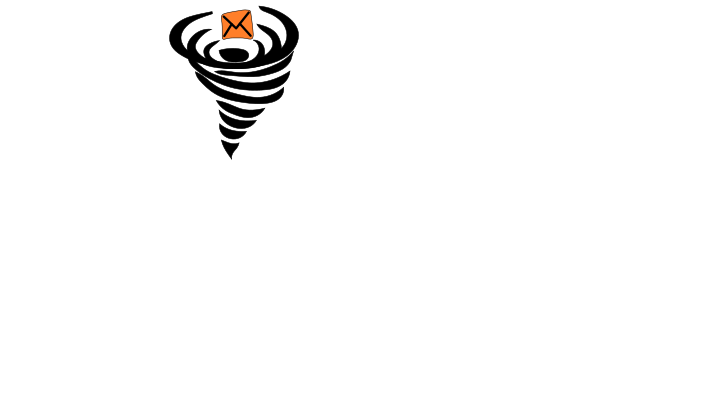
\includegraphics[height=1.1\fontcharht\font`V]{../../../../website/src/main/jbake/assets/images/MessageVortexLogo}}
\gdef\MessageVortex{\texorpdfstring{\emph{MessageVortex}}{MessageVortex}}
\gdef\VortexMessage{\emph{\defref{VortexMessage}}}
\gdef\VortexMessages{\texorpdfstring{\emph{\defref{VortexMessage}s}}{VortexMessages}}
\gdef\VortexNode{\emph{\defref{VortexNode}}}
\gdef\VortexNodes{\emph{\defref{VortexNode}s}}

% quoted environment
\usepackage{libertine}
\newcommand*\quotefont{\fontfamily{LinuxLibertineT-LF}}
\usepackage{etoolbox}
\usepackage{framed}
\newcommand*\quotesize{60} % if quote size changes, need a way to make shifts relative
% Make commands for the quotes
\newcommand*{\openquote}
{\tikz[remember picture,overlay,xshift=-4ex,yshift=-2.5ex]
	\node (OQ) {\quotefont\fontsize{\quotesize}{\quotesize}\selectfont``};\kern0pt}
\newcommand*{\closequote}[1]
{\tikz[remember picture,overlay,xshift=4ex,yshift={#1}]
	\node (CQ) {\quotefont\fontsize{\quotesize}{\quotesize}\selectfont''};}
% select a colour for the shading
\colorlet{shadecolor}{Azure}
\newcommand*\shadedauthorformat{\emph} % define format for the author argument
% Now a command to allow left, right and centre alignment of the author
\newcommand*\authoralign[1]{%
\if#1l
\def\authorfill{}\def\quotefill{\hfill}
\else
\if#1r
\def\authorfill{\hfill}\def\quotefill{}
\else
\if#1c
\gdef\authorfill{\hfill}\def\quotefill{\hfill}
\else\typeout{Invalid option}
\fi
\fi
\fi}
% wrap everything in its own environment which takes one argument (author) and one optional argument
% specifying the alignment [l, r or c]
%
\newenvironment{shadequote}[2][l]%
{\authoralign{#1}%
\ifblank{#2}%
{\def\shadequoteauthor{}\def\yshift{-2ex}\def\quotefill{\hfill}}%
{\def\shadequoteauthor{\par\authorfill\shadedauthorformat{#2}}\def\yshift{2ex}}%
\begin{snugshade}\begin{quote}\openquote}%
{\shadequoteauthor\quotefill\closequote{\yshift}\end{quote}\end{snugshade}}

% Allow byte field graphs
\usepackage{bytefield}


% Allow unbreakable hyphens
\usepackage[shortcuts]{extdash}

% set numbering for subsubsections
\setcounter{secnumdepth}{3}
\setcounter{tocdepth}{2}

% highlighting
\usepackage[bordercolor=white,backgroundcolor=gray!30,linecolor=black,colorinlistoftodos]{todonotes}
\newcommand{\hilight}[1]{\colorbox{yellow}{#1}}

% allow clever references
\usepackage{cleveref}

\gdef\shadowshift{-3pt}
\definecolor{operationcolor}{RGB}{255,226,226}
\definecolor{endoperationcolor}{RGB}{255,255,226}
\definecolor{atomicopcolor}{RGB}{217,248,217}
\definecolor{senderkeycolor}{RGB}{159, 216, 255 }
\definecolor{payloadcolor}{RGB}{233,45,64}
\definecolor{peerkeycolor}{RGB}{217,248, 217}
\definecolor{hostkeycolor}{RGB}{190,217, 232}
\definecolor{layercolor}{RGB}{190,217, 232}
\definecolor{nodecolor}{RGB}{132, 151, 176}
\definecolor{startnodecolor}{RGB}{192, 151, 176}
\definecolor{endnodecolor}{RGB}{132, 211, 176}
\definecolor{nodeshadow}{RGB}{107, 107, 107}
\definecolor{hostIdentitycolor}{RGB}{255, 226, 226 }
\definecolor{transportcolor}{RGB}{220,20,20}
\definecolor{flowColor}{RGB}{ 79,136, 187}
\definecolor{flowBorderColor}{RGB}{ 79,116, 167}
\definecolor{unrelatedcolor}{RGB}{20,220,20}

\graphicspath{{./}{inc/}{../../../../website/src/main/jbake/assets/images/}{../../../../../website/src/main/jbake/assets/images/}}

\makeatletter
\patchcmd{\backmatter}
{\@mainmatterfalse}
{\@mainmatterfalse}
{}
{}
\makeatother

\begin{document}%
%
\frontmatter%
%\newgeometry{margin=0.1cm, footskip=1mm}
\begin{titlepage}
\makeatletter
\ifdraft
	\begin{tikzpicture}[remember picture,overlay]
	  \node[rotate=60,scale=10,text opacity=0.8] at (current page.center){\color{red}\textbf{\Huge DRAFT}};
	\end{tikzpicture}
\else	
\fi
\makeatother
\pagecolor{gray}\afterpage{\nopagecolor}
\begin{center}~\\[1cm]
\includegraphics[height=0.4\paperwidth]{../../../../website/src/main/jbake/assets/images/MessageVortexLogo_huge}~\\[1cm]

% Title
\newcommand{\HRule}{\rule{\linewidth}{0.5mm}}
\HRule \\[0.4cm]
{ \huge \bfseries \makeatletter\@title\par\normalsize\@subtitle\makeatother \\[0.4cm] }

\HRule \\[4.5cm]

{\large Inauguraldissertation}\\
zur\\
Erlangung der W\"urde eines Doktors der Philosophie\\
vorgelegt der\\
Philosophisch-Naturwissenschaftlichen Fakult\"at\\
der Universit\"at Basel\\
von\\
Martin Gwerder (06-073-787)\\
von Glarus GL\\

\vfill
% Bottom of the page
{\large \today\\[1cm]}
{\footnotesize Original document available on the edoc sever of the university of Basel edoc.unibas.ch.\\[0.5cm]
\includegraphics[height=7mm]{./inc/cclic.png}~\\[0.5cm]5
This work is published under  "Creative Commons Attribution-NonCommercial-NoDerivatives 3.0 Switzerland" (CC BY-NC-ND 3.0 CH) licensed. The full license can be found at \url{http://creativecommons.org/licenses/by-nc-nd/3.0/ch/}.
}

\end{center}
\end{titlepage}

%\restoregeometry
\onecolumn
\clearpage\pagestyle{plain}

\begin{center}

Genehmigt von der Philosophisch-Naturwissenschaftlichen Fakult\"at\\
Auf Antrag von\\[0.5cm]
Prof. Dr. Christian F. Tschudin\\Prof. Dr. Heiko Schuldt\\[0.5cm]

Basel, der 18.2.2020 durch die Fakult\"atsversammlung\\[2cm]
{\rule{6cm}{0.2pt}\\ Prof. Dr. Martin Spiess}
\end{center}
\clearpage



\section*{\abstractname}   
\myabstract

\vspace*{\fill}

\section*{Acknowledgments}
I want to thank my wife Cornelia and my lovely three kids (Saphira, Florian, and Aurelius) for their patience and their support. Without them I could never have done this work.

I want to thank Prof. Dr. C. Tschudin and the University of Basel for the possibility of writing this work and for the challenges they opposed to me, allowing me to grow. 

Dr. Andreas Hueni for his thoughts and challenging outside-the-normal-box thinking.

Prof. Dr. Carlos Nicolas of the University of Northwestern Switzerland for being such a valuable sparring partner allowing me to test my ideas.

I want to acknowledge all the individuals who have coded for the \LaTeX project for free. It is due to their efforts that we can generate professionally typeset PDFs (and far more) for free.






%!TeX program=pdflatex
%!TeX encoding=utf8
%!TeX spellcheck = en_US
%!TeX root = ../../messageVortex.tex

\cleardoublepage
\makeatletter
\renewcommand{\@pnumwidth}{4em}
\renewcommand*\l@section{\@dottedtocline{1}{1.5em}{3em}}
\renewcommand*\l@subsection{\@dottedtocline{2}{3.8em}{3.8em}}
\renewcommand*\l@subsubsection{\@dottedtocline{3}{7.4em}{5em}}
% Special Part
\renewcommand*\l@part[2]{%
	\ifnum \c@tocdepth >-2\relax
	\addpenalty{-\@highpenalty}%
	\addvspace{2.25em \@plus\p@}%
	\setlength\@tempdima{3em}%
	\begingroup
	\parindent \z@ \rightskip \@pnumwidth
	\parfillskip -\@pnumwidth
	\begin{tcolorbox}[colback=head, right=0ex, left=0cm, sharpish corners, boxrule=0mm, width=1.0\textwidth]
		{\leavevmode
			\large \bfseries \vbox{\color{white}\sffamily\bfseries#1}%
			\hb@xt@0ex{\color{white}\hss #2}
		}
	\end{tcolorbox}
	\vspace*{1ex}
	\nobreak
	\global\@nobreaktrue
	\everypar{\global\@nobreakfalse\everypar{}}%
	\endgroup
	\fi}
\makeatother

\pagestyle{scrheadings}

\onecolumn
%\setpnumwidth{2em}
%\setlength\cftsectionnumwidth{3em}
\setcounter{tocdepth}{4}
\tableofcontents

\newpage
\indexes
%\twocolumn

\makeatletter
\newlength\mylena
\newlength\mylenb
\setlength\mylena{1.3cm}
\setlength\mylenb{\dimexpr\columnwidth-\mylena\relax}

\newcommand\PlaceNumber[1]{%
	\makebox[\mylena][l]{#1}}

\titleformat{\chapter}
{\Large\sffamily\bfseries}
{}
{0em}
{\PlaceNumber{\thechapter}\parbox[t]{\mylenb}{\raggedright#1}}

\titlespacing*{\chapter}{0pc}{3ex \@plus4pt \@minus3pt}{5pt}

\titleclass{\chapter}{straight}%% added
\makeatother



\mainmatter
\startcontents
%!TeX program=pdflatex
%!TeX encoding=utf8
%!TeX spellcheck = en_US
%!TeX root = ../../messageVortex.tex

\part{Introduction}
\chapter{Foreword}
Almon Brown Strowger was the owner of a funeral parlor in St. Petersburg. He filed a patent on March \nth{10}, 1891 for an ``Automatic Telephone Exchange'' \cite{pulseDialingPatent}. This patent built the base for modern automated telephone systems. According to several sources, he was annoyed by the fact that the local telephone operator was married to another undertaker. She diverted potential customers of Mr. Strowger to her husband instead, which caused Almon B. Strowger to lose business. In 1922, this telephone dialing system, which is nowadays called pulse dialing became the standard dialing technology for more than 70 years until tone dialing replaced it.

This dialing technology enabled automatic messaging for voice and text messages (e.g., telex) up until today and is the foundation for current routed networks. These networks build the base for our communication-based Society these days and allow us to connect quickly with any person or company of our wish. We use these networks today as communication meaning for all purposes, and most of the people spend minimal thoughts on the possible consequences arising if someone puts hands on this communication. 

Collected data may be used to judge our intentions and thus is not only confidential if we have something to hide. This problem has dramatically increased in the last years as big companies and countries started to collect all kinds of data and created the means to process them. It allows supposedly to judge peoples not only on what they are doing but as well, on what they did and what they might do. Numerous events in the present and past show that multiple actors, some of which are state-sponsored, collected data on a broad base within the internet. Whether this is a problem or not may be a disputable fact. Undisputed is, however, that such data requires careful handling and accusations should then base on solid facts. Unacceptable seems the use of "guesses" or "extrapolations." 

To show that this may happen even under complete democratic control we might refer to events such as the ``secret files scandal'' (or  ``Fichenskandal'') in Switzerland. In the years from 1900 to 1990 Swiss government collected 900’000 files in a secret archive (covering roughly 10\% of the natural and juristic entities within Switzerland at that time). More about the Fichenskandal is well documented in the Swiss Federal Archives (https://www.bar.admin.ch).

Whistleblower Edward Snowden leaked a vast amount of documents suggesting that such attacks on privacy are commonly made on a global scale. The documents leaked in 2009 by him claim that there was a data collection starting in 2010. Since these documents are not publicly available, it is hard proving the claims based on these documents. However -- A significant number of journalists from multiple countries screened these documents, the information seems credible. According to these documents (verified by \href{http://www.nrc.nl/nieuws/2013/11/23/nederland-sinds-1946-doelwit-van-nsa}{NRC}), NSA infiltrated more than 50k computers with malware to collect classified or personal information. They furthermore infiltrated Telecom-Operators (mainly executed by British GCHQ) such as Belgacom to collect data and targeted high member of governments even in associated states (such as the mobile phone number of Germany's president). A later published shortened list of ``selectors'' in Germany showed 68 telephone and fax numbers targeting economy, finance and agricultural parts of the German government. A global survey done by the freedom house\cite{FOTN2018} claims a decrease in internet freedom for the \th{8} year in a row. 

This list of events shows that big players are collecting and storing vast amounts of data for analysis or possible future use. The list of events also shows that the use of this data has in the past been at least partially questionable. As a part of possible, this work analyses the possibility of using state-of-the-art technology to minimize the information footprint of a person on the Internet. 

We leave a large information footprint in our daily communication. On a regular email, we disclose everything in an ``postcard'' to any entity on its way. Even when encrypting a message perfectly with today's technology (S/MIME\cite{RFC2045} or PGP\cite{RFC2015}) it still leaves at least the originating and the receiving entity disclosed, or we rely on the promises of a third party provider which offers a proprietary solution. Even in those cases, we leak pieces of information such as ``message subject'', ``frequency of exchanged messages'', ``size of messages'', or ``client being used''. A suitable anonymity protocol has therefore far more attributes to cover than the message itself. It includes besides the message itself, all metadata, and all the traffic flows. Furthermore, a protocol to anonymize messages should not rely on the trust of infrastructure other than the infrastructure under control of the sending or receiving entity. Trust in any third party might be misleading in terms of security.

Central infrastructure is bound to be of particular interest to anyone gathering data. It may furthermore allow manipulating the system or the data or the data flow. So, avoiding a central infrastructure is a good thing.

Leaving no information trail when sending information from one person to another is hard to achieve. Most messaging systems disclose at least the peer partners when sending messages. Metadata such as starting and endpoints, frequency, or message size are leaked in all standard systems even when encrypting messages.

Allowing an entity to collect data may affect senders and recipients of any information. Collection of vast amounts of data allows a potent adversary to build a  profile of a person. Unlike in the past, the availability of this kind of information has been risen to a never known extend with the internet.

An entity in possession of such Profiles may use them for many purposes. These include service adoption, directed advertising, or classification of citizens. The examples given above show that the effects of this data is not limited to the internet but reaches us effectively in the real world.

The main problem of this data is that it may be collected over a considerable amount of time and evaluated at any time. It even happened that standard practices of time are differently judged upon in a later time. Persons may then be judged retrospectively upon these types of practice. This questionable type of judgment is visible in the tax avoidance discussion. 

People must be able to control their data footprint. Not providing these means does effectively allow any country or a more prominent player to ban and control any number of persons within or outside the internet. 

In this work, a new protocol is designed to allow message transfer through existing communication channels. These messages are next to unobservable to any third party. This unobservability does not only cover the message itself but all metadata and flows associated with it. We called this protocol ``MessageVortex'' or in short just ``Vortex''. The protocol is designed in such a way so that it is capable of using a wide variety of transport protocols. It is even possible to switch protocols while the messages are in the transfer. This behavior allows media breaches (at least on a protocol level) and makes analysis even harder.

The new protocol allows secure communication without the need for trusting the underlying transport media. Furthermore, the usage of the protocol itself is possible without altering the immediate behavior of the transport layer. That way it is possible to use the transport layers regular traffic to increase the noise in which information has to be searched. 

This work splits into multiple parts. In the first part, we collect available researches and technologies. We emphasize in all technologies on the strength and weaknesses relevant to this work. 

In the second part, we reassemble the parts to a new protocol. 

In the third part, we analyze the protocol for the fitness of the purpose. We try to find weaknesses and work out recommendations for protocol usage. 

In the last part, we discuss the results and try to summarize the findings. We furthermore elaborate to what extent the protocol fulfills the requirements mentioned in the previous sections.

\section{Contributions}
This thesis contributes to the topic in the following senses:
\begin{itemize}
	\item It introduces a consistent model for message delivery, which includes all endpoints and involved parties.
	\item It shows an approach based on existing protocols for anonymous communication, which gives full control of the anonymity to the sender while controlling the costs.
	\item It offers a client application implementing the proposed Protocol as IMAPv4 cache daemon and as SMTP relay.
\end{itemize}

\chapter{Notation}
\section{Cryptography \label{sec:encNot}}
The theory in this document is heavily based on symmetric encryption, asymmetric encryption, and hashing. To use a uniformed notation I use $E^{K_a}(M)$ (where $a$ is an index to distinguish multiple keys) resulting in $\mathbf{M^{K_a}}$ as the encrypted message. If we are reflecting a tuple of information, we write it in boldface. To express the content of the tuple, we use angular brackets $\mathbf{L\langle normalAddress,vortexAddress\rangle }$. If we want Messages encrypted with multiple keys do list the used keys as a comma-separated list in superscript $E^{K_b}\left(E^{K_a}\left(M\right)\right)=M^{{K_{a}},{K_b}}$.

For a symmetric encryption of a message $\mathbf{M}$ with a key $K_a$ resulting in $\mathbf{M^{K_a}}$ where $a$ is an index to distinguish different keys. Decryption uses therefore $D^{K_a}(\mathbf{M^{K_a}})=\mathbf{M}$.

As notation for asymetric encryption we use $E^{K^{1}_a}(\mathbf{M})$ where as $K^{-1}_a$ is the private key and $K^{1}_a$ is the public key of a key pair $K^p_a$. The asymmetric decryption is noted as $D^{K^{-1}_a}(\mathbf{M})$.

For hashing, we do use $H(\mathbf{M})$ if unsalted and $H^{S_a}$ if using a salted hash with salt $S_a$. The generated hash is shown as $H_M$ if unsalted and $H^{S_a}_M$ if salted.

If we want to express what details contained in a tuple we use the the notation $\mathbf{M\langle t,MURB,serial\rangle }$ respectively if encrypted $\mathbf{M^{K_{a}}\langle t,MURB,serial\rangle}$.

\begin{align*}
\text{asymetric:}         & E^{K^{-1}_a}\left(\mathbf{M}\right)                        	&& =\mathbf{M}^{K^{-1}_a}\\
                          & D^{K^{1}_a}\left(E^{K^{-1}_a}\left(\mathbf{M}\right)\right)	&& =\mathbf{M}\\
                          & D^{K^{-1}_a}\left(E^{K^{1}_a}\left(\mathbf{M}\right)\right)	&& =\mathbf{M}\\
\text{symetric:}          & E^{K_a}\left(\mathbf{M}\right)                             	&& =\mathbf{M}^{K_a}\\
      		              & D^{K_a}\left(E^{K_a}\left(\mathbf{M}\right)\right)          && =\mathbf{M}\\
\text{hashing (unsalted):}& H\left(\mathbf{M}\right)                                   	&& =\mathbf{H}_M\\
\text{hashing (salted):}  & H^{S_a}\left(\mathbf{M}\right)                             	&& =\mathbf{H}^{S_a}_M
\end{align*}

In general, subscripts denote selectors to differentiate the values of the same type, and superscript denotes relevant parameters to operations expressed. The subscripted and superscripted information may be omitted where not needed.

We refer to the components of a Vortex Message as follows:
\begin{align*}
\text{Prefix component:}         & \mathbf{PREFIX}             	&=D^{K^{1}_a}\left(\mathbf{P}^{K^{-1}_a}\right) &=D\left(\mathbf{P}\right)\\
\text{Header component:}         & \mathbf{HEAD}             	&=D^{K^{1}_a}\left(\mathbf{H}^{K^{-1}_a}\right) &=D\left(\mathbf{H}\right)\\
\text{Route component:}         & \mathbf{ROUTE}             	&=D^{K^{1}_a}\left(\mathbf{R}^{K^{-1}_a}\right) &=D\left(\mathbf{R}\right)\\
\end{align*}

In general, a decrypted Block is written as capitalized multi-character boldface. An encrypted Block is expressed as capitalized single character boldface.

\section{Code and commands}
We write code blocks as a light grey block with line numbers:

\begin{lstlisting}
public class Hello {
  public static void main(String args[]) {
    System.println("Hello. "+args[1]);
  }
}
\end{lstlisting}

Commands entered at the command line are in a grey box with a top and bottom line. Whenever root rights are required the command line is prefixed with a ``\#''. Commands not requiring specific rights are prefixed with a ``\$''. Lines without a trailing ``\$'' or ``\#'' are output lines of the previous command. If long lines have to be broken to fit into the paper a ``$\hookleftarrow$'' is inserted to indicate that the line break has been introduced for readability.

\begin{lstlisting}[language=bash]
# su -
# javac Hello.java 
# exit
$ java Hello
Hello.
$ java Hello "This is a very long command-line that had to be broken to fit into the code box displayed on this page."
Hello. This is a very long command-line that had to be broken to fit into the code box displayed on this page.
\end{lstlisting}

\section{Hyperlinking}
The electronic version of this document is hyperlinked. References to the glossary or the literature may be clicked to find the respective entry. Chapter or table references are clickable too. 

\chapter{Main Research Question}
The main topic of this thesis was defined as follows:
\begin{itemize}
	\item Is it possible to have specialized messaging protocol used on the Internet based on ``state of the science'' technologies offering a high level of unlikability (sender and receiver anonymity) towards an adversary with a high budget and privileged access to internet infrastructure?
\end{itemize}

Based on this central question there are several sub questions grouped around various topics:

\begin{enumerate}
	\item What technologies and methods may be used to provide sender and receiver anonymity and unlinkability when sending messages against a potential adversary? (SQ1)
	\item How can entities utilizing MessageVortex be attacked, and what measures are available to circumvent such attacks? (SQ2)
	\item How can attacks target anonymity of a sending or receiving entity be mitigated by design within MessageVortex? (SQ3)
\end{enumerate}

\section{SQ1: Technologies for sending messages maintaining unlinkability against an adversary}
This question covers the principal part of the work. We try to elaborate a first rough list of criteria for the MessageVortex protocol. We then create a list of suitable technologies. Based on this list, we define a protocol combining these technologies and researches to a solution. This solution is implemented and analyzed for suitability based on the criteria defined.

\section{SQ2: Attacking unlinkability and circumvention}
Within this question, we look at various attacks and test resistance of the protocol based on the definition of the protocol. We do this by first collecting well-known attacks (either generic or specific to a technology used in the protocol). We then try to elaborate if these attacks might be successful (and if so under what circumstances).

\section{SQ3: Attack Mitigation by design}
Within this question, we define baselines to mitigate attacks by defining guidelines for using the protocol. We analyze the effectiveness of the guidelines and try to elaborate on the general achievement level of the protocol by looking at the criteria defined in SQ1. 

This question is answered in part \ref{sec:discussion}.
%!TeX program=pdflatex
%!TeX encoding=utf8
%!TeX spellcheck = en_US
%!TeX root = ../../messageVortex.tex

% ********************************************************************************************************
% *** Intro to MessageVortex
% ********************************************************************************************************
% ********************************************************************************************************
% *** Research Preexisting work
% ********************************************************************************************************
\part{Concepts and Techniques}
\fxwarning{complete section}

\chapter{Anonymity Research}
In this section, we collect protocols research related to anonymity. We did not stick to anonymous message transfer. Instead, we took a broad focus in terms of technology and outlined in each protocol strengths and weaknesses identified, which may be relevant to this research.

\section{Definition of Anonymity}
As the definition for Anonymity we take the definition as specified in \cite{anonTerminology}.\DeclareFixedFootnote{\omitted}{footnotes omitted in quote}
\begin{quote}
	Anonymity of a subject means that the subject is not identifiable within a set of subjects, the anonymity set.\omitted
\end{quote}
and
\begin{quote}
	Anonymity of a subject from an attacker's perspective means that the attacker cannot sufficiently identify the subject within a set of subjects, the anonymity set.\omitted
\end{quote}

We define the anonymity set as the set of all possible subjects within a supposed message. The anonymity of a subject towards an observing third party is a crucial factor as it relates directly to our adversary model.

\section{\texorpdfstring{$k$}{k}-Anonymity}
$k$-anonymity is a term introduced in \cite{k-anonymous:ccs2003}. This work claims that entities are not responsible for an action if an observer is unable to match a specific action to less than $k$ entities.

The Document distinguishes between \textit{Sender $k$-anonymity}, where the sending entity can only be narrowed down to a set of $k$ entities and \textit{Receiver $k$-anonymity}. 

The size of $k$ is a crucial factor. One of the criteria is the legal requirements of the jurisdiction. Depending on the jurisdiction, it usually is not possible to prosecute someone if an action is not directly coupled to one person. Another criterion might be the decreasing of $k$ over time. If a Vortex account is used, we have to assume that some vortex identities go out of commission over time. If $k$ is chosen according to a legal requirement, it should be taken into account that $k$ might be decreasing over time.

\section{\texorpdfstring{$\ell$}{l}-Diversity}
In \cite{machanavajjhala2007diversity} an extended model of $k$-anonymity is introduced. In this paper, the authors emphasize that it is possible to break a $k$-anonymity set if there is additional information available which may be merged into a data set so that a distinct entity can be filtered from the $k$-anonymity set. In other words, if an anonymity set is to tightly specified, additional background information might be sufficient to identify a specific entity in an anonymity set.

It might be arguable that a $k$-anonymity in which a member is not implicitly $k$-anonymous still is sufficient for $k$-anonymity in its sense. However, the point made in this work is right and is taken into account. Their approach is to introduce an amount of invisible diversity into $k$-anonymous sets, so that common background knowledge is no longer sufficient to isolate a single member.

\section{\texorpdfstring{$t$}{t}-Closeness}
While $\ell$-diversity protects the identity of an entity, it does not prevent information gain. A subject which is in a class has the same attributes. This is where $t$-closeness\cite{li2007t} comes into play. $t$-closeness is defined as follows:

\begin{quote}
	An equivalence class is said to have $t$-closeness if the distance between the distribution of a sensitive attribute in this class and the distribution of the attribute in the whole table is no more than a threshold. A table is said to have $t$-closeness if all equivalence classes have $t$-closeness.
\end{quote}

\section{Single Use Reply Blocks and Multi-Use Reply Blocks}
Chaum first introduced the use of reply blocks in \cite{CHAUM1}. A routing block, in general, is a structure allowing to send a message to someone without knowing the targets' real address. Reply blocks may be differentiated into two classes ``Single Use Reply Blocks'' (SURBs)  and ``Multi-Use Reply Blocks'' (MURBs). SURBs may be used once while MURBs may be used a limited number of times. 

Within our research, we discovered that if a routing protocol is reproducible, the traffic of a MURB may be used to identify some of the properties of the message. Depending on the type of attack, the block has to be repeated very often. For this reason, we limited the number of replays to a low number. The concept is that we have, in our case a routing block, which might be used up to $n$ times ($0<n<127$). It is easily representable in a byte integer (signed or unsigned) on any system. It is big enough to support human communication sensibly and is big enough to add not too much overhead when rerequesting more MURBs. The number should not be too big because if a MURB is reused, the same pattern of traffic is generated, thus making the system susceptible to statistical attacks.

\section{Censorship}
As a definition for censorship we take
\begin{quote}
	Censorship: the cyclical suppression, banning, expurgation, or editing by an individual, institution, group or government that enforce or influence its decision against members of the public -- of any written or pictorial materials which that individual, institution, group or government deems obscene and ``utterly without redeeming social value,'' as determined by ``contemporary community standards.''
\end{quote}

The definition is attributed to Chuck Stone Professor at the School of Journalism and Mass Communication, University of North Carolina. Please note that ``Self Censorship'' (not expressing something in fear of consequences) is a form of censorship too.

In our more technical we reduce the definition to
\begin{quote}
	Censorship: A systematic suppression, modification, or banning of data in a network by either removal, or modification of the data, or systematic influencing of entities involved in the processing (e.g., by creating, routing, storing, or reading) of this data.
\end{quote}
This simplified definition narrows down the location to the Internet as it is the only relevant location for us.  Furthermore, it limits the definition to the maximum reach within that system.

\subsection{Censorship Resistant}
A censorship-resistant system is a system that allows the entities of the system and the data itself to be unaffected from censorship. Please note that this does not deny the presence of censorship per se. It still exists outside the system. However, it has some consequences for the system itself.

\begin{itemize}
	\item The system must be either undetectable or out of reach for an entity censoring.\\
	The possibility of identifying a protocol or data allows a censoring entity to suppress the use of the protocol itself. 
	\item The entities involved in a system must be untraceable.\\
	Traceable entities would result in a mean of suppressing real-world entities participating in the system.
\end{itemize}

\subsection{Parrot Circumvention}
In \cite{oakland2013-parrot} \citeauthor{oakland2013-parrot} express that it is easy for a human to determine decoy traffic as the content is easily identifiable as generated content. While this is true, there is a possibility here to generate ``human-like'' data traffic to a certain extent. As an adversary may not assume that his messages are replied to, the problem does not boil down to a true Turing test. It remains on a ``passive observer Turing test'', enabling the potential nodes to choose their messages. 

In our design, this is the job covered by the blending layer. The blending layer generates these messages. These messages are context-less or remain in the context of previous conversations.

\subsection{Censorship Circumvention}
Several technical ways have been explored to circumvent censorship. All seem to boil down to the following main ideas:
\begin{itemize}
	\item Hide data
	\item Copy or distribute data to a vast amount of places to improve the lifespan of data
	\item Outcurve censorship measurements
\end{itemize}

In the following section, we look at technologies and ideas dealing with these circumvention technologies.

\subsubsection{Covert Channel and Channel Exploitations}
The original term of covert channels was defined by \citeauthor{Lampson73anote}\cite{Lampson73anote} as 

\begin{quote}
	not intended for information transfer at all, such as the service program's effect on system load.
\end{quote}

This was defined  in such a way to distinguish the message flow from 

\begin{quote}
	legitimate channels used by the confined service, such as the bill.
\end{quote}

The use of a legitimate channel such as \defref{SMTP} and hide information within this specific channel is not a usage of a covert channel. We refer to this as channel exploitation.

\subsubsection{Steganography}

Steganography is an important part when it comes to unlinking information. In \cite{6828087} and \cite{subhedar2014current} we get a very rough overview. As some of the types and algorithms address specific topics of steganography (e.g., some hide from automatic detection and others address a human message stream auditor), we need to choose carefully. In our specific case, the main idea is to hide within the sheer mass of Internet traffic. As a human auditor screening all the messages is a minor thread, we focus on machine-based censorship. Most of the images sent in \defref{SMTP} are jpg images (see table \ref{tab:emailAttachments} on page \pageref{tab:emailAttachments}). We limited our search to algorithms capable of hiding binary data within these files. The number of academically researched options was surprisingly low.

After reviewing the options, we decided to go for F5\cite{f5}. It is a reasonably well-researched algorithm which attracted many researchers. The original F5 implementation had a detectable issue with artifacts\cite{F5broken} caused by the recompression of the image. This issue was caused only due to a problem in the reference implementation, and the researchers have provided a corrected reference implementation without the weakness.

% We use https://github.com/matthewgao/F5-steganography

YASS, as described in \cite{solanki2007yass}, was not considered a candidate. Although less researched, researchers found multiple weakness\-es\cite{kodovsky2010modern,li2009steganalysis}.

\subsubsection{Timing Channels}

Timing channels are a specialized form of covert channels. In timing channels, the information itself hides not within the data of the channel, but the usage of the channel is in such a way that it is capable of reflecting the data. As we do not have control over the timing of the transport channel, this is not an option for us.

\chapter{Cryptography}

Whenever dealing with obfuscating data and maintaining the integrity of data, cryptography is the first tool in the hand of an implementer. A vast amount of research in this area does already exist. For this work, we focussed on algorithms either very well researched and implemented or research, which seem very valuable when putting this work into place. 

In symmetric encryption in this paper always assumes that
\begin{eqnarray}
D^{K_a}\left(E^{K_a}\left(\mathbf{M}\right)\right) & = & \mathbf{M}
\end{eqnarray} 

For a key $K_b\neq K_a$ this means

\begin{eqnarray}
D^{K_a}\left(E^{K_b}\left(\mathbf{M}\right)\right) & \neq & \mathbf{M}\\
D^{K_b}\left(E^{K_a}\left(\mathbf{M}\right)\right) & \neq & \mathbf{M}
\end{eqnarray} 

The following candidates have been analyzed:
\begin{itemize}
	\item AES\\
	NIST announced AES in \citeyear{standard2001announcing} as a result of a contest. The algorithm works with four operations (subBytes, ShiftRows, mixColumns, and addRoundKey). These operations are repeated depending on the key length 10 to 14 times. 
	
	AES is up until now (2018) unbroken. It has been weakened in the analysis described in \cite{tao2015improving}, which reduces the complexity by roughly one to two bits. 
	
	\item Camellia\\
	The camellia algorithm is described in \cite{RFC3713}. The key sizes are 128, 192, and 256. Camellia is a Feinstel cipher with 18 to 24 rounds depending on the key size. Up until today, no publication claims break this cipher. 
\end{itemize}

For all asymmetric encryption algorithm in this paper, we may assume that\ldots

\begin{eqnarray}
D^{K^{-1}_a}\left(E^{K^{1}_a}\left(\mathbf{M}\right)\right) & = & \mathbf{M}\\
D^{K^{1}_a}\left(E^{K^{-1}_a}\left(\mathbf{M}\right)\right) & = & \mathbf{M}
\end{eqnarray} 

It is important that 
\begin{eqnarray}
D^{K^{-1}_a}\left(E^{K^{-1}_a}\left(\mathbf{M}\right)\right) & \neq & \mathbf{M}\\
D^{K^{1}_a}\left(E^{K^{1}_a}\left(\mathbf{M}\right)\right)   & \neq & \mathbf{M}
\end{eqnarray} 

And for any other Keypair $K^{p}_a \neq K^{p}_b$
\begin{eqnarray}
D^{K^{-1}_b}\left(E^{K^{1}_a}\left(\mathbf{M}\right)\right)  & \neq & \mathbf{M}\\
D^{K^{1}_b}\left(E^{K^{1}_a}\left(\mathbf{M}\right)\right)   & \neq & \mathbf{M}\\
D^{K^{-1}_b}\left(E^{K^{-1}_a}\left(\mathbf{M}\right)\right) & \neq & \mathbf{M}\\
D^{K^{1}_b}\left(E^{K^{-1}_a}\left(\mathbf{M}\right)\right)  & \neq & \mathbf{M}
\end{eqnarray} 

The number of crypto algorithms was higher than the steganography options. When looking for well-researched algorithms basing on different mathematical problems and having well-defined outlines, numbers dropped dramatically again.

\begin{itemize}
	\item RSA\\
	In \citeyear{Rivest:1978:MOD:359340.359342} the authors \citeauthor{Rivest:1978:MOD:359340.359342} published with \cite{Rivest:1978:MOD:359340.359342} a paper which did revolutionize cryptography for years. In their paper, the authors described an encryption method later to be called RSA, which required a key pair ($K_a$) referenced as public ($K^{1}_a$) and private keys ($K^{-1}_a$). The novelty of this system was that anything encrypted with the public key was only decryptable with the private key and vice versa.
	
	RSA is up until the day of writing this paper not publicly know to be broken (unless a too small key size is used). However -- \citeauthor{Shor97polynomial-timealgorithms} described in \citeyear{Shor97polynomial-timealgorithms} an algorithm which should enable quantum computers to break RSA far faster than done with traditional computers. In the section \ref{sec:keySize} we do elaborate these effects further.
	\item ECC\\
	The elliptic curves were independently suggested by \cite{Miller1986} and \cite{Koblitz04guideto} in 1986. Elliptic curve Cryptography started to be widely deployed in the public space in 2006. Since then, it seems to compete very well with the well established RSA algorithm. While being similarly well researched ECC, has the advantage of far shorter key sizes for the same grade of security.
	\item McElliece\\
	McEliece was first implemented and then removed again. The key size to gain equivalent security to RSA1024 was $\approx 1MB$. This was impractical and thus discarded again. This was done, although there is up until now no known quantum capable algorithm reducing the key size of McEliece.
	\item NTRU\\
	In \cite{Hoffstein1998} \citeauthor{Hoffstein1998} described the NTRU algorithm. The inclusion of this algorithm was disputed as it is patented in the united states as US7031468. It was included because the company Security Innovation holding the patent, released the NTRU algorithm on March \thanks{28} 2018 into the public domain according to a blog entry on the company website. While NTRU is not as well researched as RSA, it has been around for more than 20 years without being significantly affected by known attacks.
	\item ElGammal\\
	We rejected ElGamal as a cryptosystem to include. It bases on the same mathematical problems for cryptoanalysis as RSA (discreet logarithms) but is not as common as RSA.
\end{itemize}


\section{Homomorphic encryption}
Homomorphic encryption, as introduced in \cite{feldman1987practical}, was from the beginning a strong candidate to be used within our work. Unfortunately, we did not find a way to apply the core addRedundancy operation in homomorphic encryption. Transforming the original data to the GF space in an efficient way to apply matrices was not doable and thus rejected.

%\cite{Gentry:2009:FHE:1536414.1536440} %FIXME dangling reference

\section{Deniable Encryption and Deniable Steganography}

Deniable encryption and deniable steganography have been considered out-of-bounds for this work. The main reason is that the presence of encryption (which is not deniable in both cases) may be sufficient for a censor to block a message. Adding a layer to make sure that encryption or steganography is deniable, does not add valuable properties to our system as the sheer presence of encryption might be sufficient for censorship. 

\section{Key Sizes\label{sec:keySize}}

The question of key sizes is hard to answer as it depends on the current and future possibilities of an adversary, which is again depending on not foreseeable research. We tried to collect a couple of recommendations.

\href{http://www.ecrypt.eu.org/}{Encrypt II (http://www.ecrypt.eu.org/)} recommends currently for a ``foreseeable future'' 256 Bits for symmetric encryption and for asymmetric encryption based on factoring modulus 15424 Bits. Elliptic Curve Cryptography and Hashing should be sufficient if used with at least 512 Bits. If the focus is reduced to the next $\approx$ 20 years, then the key size recommendations are reduced to 128 Bit for symmetric encryption, 3248 Bits for factoring modulus operations, and 256 Bits for elliptic curves and hashing.

According to the equations proposed by \citeauthor{Lenstra04keylength.} in \cite{Lenstra04keylength.} an asymmetric key size of 2644 Bits respectively symmetric key length of 95 Bits, or 190 Bits for elliptic curves and hashing should be sufficient for security up to the year 2048. 

According to \cite{CNSASuite} (superseding well known and often used \cite{nsa-fact-sheet-B}) data classified up to ``top secret'' should be signed with RSA 3072+ or ECDSA P-384.  For symmetric encryption, they recommend AES 256 Bits, for Hashing at least SHA-384 and for Elliptic curves a 384 Bit sized key.

As it might seem not a wise idea to consider the recommendation of a potential state-sponsored adversary and the Formulas proposed by \citeauthor{Lenstra04keylength.} do not explicitly take quantum computers into account, we follow the advice of ENCRYPT II.

Furthermore, taking all recommendations together, it seems that all involved parties assume the most trust in elliptic curves rather than asymmetric encryption based on factoring modulus.

\section{Cipher Mode}
The cipher mode defines how multiple blocks encrypted with the same key are handled. Main characteristics of cipher modes to us are:
\begin{itemize}
	\item Parallelisable\\ 
	Can multiple parts of a plaintext be encrypted simultaneously? This feature is important for multi CPU and multi-core systems as they can handle parallelizable more efficiently by distributing them on multiple CPUs.
	\item Random access in decryption\\
	Random access on decryption allows efficient partial encryption of a ciphertext.
	\item Initialisation vector\\
	An initialization vector has downsides and advantages. On the downsides is the fact that an initialization vector must be shared with the message or before distributing it. It is essential to understand that the initialization vector itself usually is not treated as a secret. It is not part of the key.
	\item Authentication\\
	Authentication guarantees that the deciphered plaintext has been unmodified since encryption. It does not make a statement over the identity of the party encrypting the text. Such an identifying authentication is referred to as signcryption.
\end{itemize}

We evaluated the most common cipher modes for suitability. For MessageVortex, we focussed on modes that have the properties parallelizable, random access, and do not do authentication. The main focus, besides the characteristics mentioned above, was on the question of whether there is an open implementation available in java, which is reasonably tested.

\begin{itemize}
	\item ECB (Electronic Code Book)\\
	ECB is the most basic mode. Each block of the cleartext is encrypted on its own. This results in a big flaw: blocks containing the same data will always transform to the same ciphertext. This property makes it possible to see some structures of the plain text when looking at the ciphertext. This solution allows the parallelization of encryption, decryption, and random access while decrypting. Due to these flaws, we rejected this mode.
	\item CBC (Cypher Block Chaining)\\  
	CBC extends the encryption by xor'ing an initialization vector into the first block before encrypting. For all subsequent blocks, the ciphertext result of the preceding block is taken as xor input. This solution does not allow parallelization of encryption, but decryption may be paralleled, and random access is possible. As another downside, CBC requires a shared initialization vector. As with most IV bound modes, an IV/key pair should not be used twice, which has implications for our protocol.
	\item PCBC (Propagation Cypher Block Chaining)\\
	CBC extends the encryption by xor'ing, not the ciphertext but a xor result of ciphertext and plaintext. This modification denies parallel decryption and random access compared to CBC.
	\item EAX\\      
	EAX has been broken in 2012\cite{minematsu2013attacks} and is therefore rejected for our use.
	\item CFB (Cypher Feedback)
	CFB is specified in \cite{dworkin2001recommendation} and works precisely as CBC with the difference that the plain text is xor'ed and the initialization vector, or the preceding cipher result is encrypted. CFB does not support parallel encryption as the ciphertext input from the preceding operation is required for an encryption round. CFB does, however, allow parallel decryption and random access.
	\item OFB\\
	\cite{dworkin2001recommendation} specifies OFB and works exactly as CFB except for the fact that not the ciphertext result is taken as feedback but the result of the encryption before xor'ing the plain text. This denies parallel encryption and decryption, as well as random access.
	\item OCB (Offset Codebook Mode)\\
	This mode was first proposed in \cite{rogaway2003ocb} and later specified in \cite{krovetz-ocb-04}. OCB is specifically designed for AES128, AES192, and AES256. It supports authentication tag lengths of 128, 96, or 64 bits for each specified encryption algorithm. OCB hashes the plaintext of a message with a specialized function $H_{OCB}(\mathbf{M})$. OCB is fully parallelizable due to its internal structure. All blocks except the first and the last can be encrypted or decrypted in parallel.
	\item CTR\\
	CTR is specified in \cite{lipmaa2000ctr} and is a mixture between OFB and CBC. A nonce concatenated with a counter incrementing on every block is encrypted and then xor'ed with the plain text. This mode allows parallel decryption and encryption, as well as random access. Reusing IV/Key-pairs using CTR is a problem as we might derive the xor'ed product of two messages. This problem only applies where messages are not uniformly random such as in an already encrypted block.
	\item CCM\\
	Counter with CBC-MAC (CCM) is specified in \cite{RFC3610}. It allows to pad and authenticate encrypted and unencrypted data. It furthermore requires a nonce for its operation. The size of the nonce is dependent on the number of octets in the length field. In the first 16 bytes of the message, the nonce and the message size is stored. For the encryption itself, CTR is used. It shares the same properties as CTR. 
	
	It allows parallel decryption and encryption as well as random access.
	\item GCM (Galois Counter Mode)\\
	GCM has been defined in \cite{mcgrew2004galois}, and is related to CTR but has some major differences. The nonce is not used (just the counter starting with value 1). To authenticate the encryption, an authentication token $auth$ is hashed with $H_{GFmult}$ and then xor'ed with the first cipher block. All subsequent cipher blocks are xor'ed with the previous result and then hashed again with $H_{GFmult}$. After the last block the output $o$ is processed  as follows: $H_{GFmult}(o\bigoplus (len(A)||len(B))) \bigoplus E^{K^0}(counter_0)$. As a result, GCM is not parallelizable and does not support random access.
	
	The mode has been analyzed security-wise in \citeyear{mcgrew2004security} and showed no weaknesses in the analyzed fields \cite{mcgrew2004security}. 
	
	GCM supports parallel Encryption and decryption. Random access is possible. However, authentication of encryption is not parallelizable. The authentication makes it unsuitable for our purposes. Alternatively, we could use a fixed authentication string.
	\item XTS (XEX-based tweaked-codebook mode with ciphertext stealing)\\
	This mode is standardized in IEEE 1619-2007 (soon to be superseded). A rough overview of XTS may be found at \cite{Martin2010}. It was developed initially for Disks offering random access and authentication at the same time. 
	\item CMC (CBC-mask-CBC) and EME (ECB-mask-ECB)\\ 
	In \cite{Halevi:2003} \citeauthor{Halevi:2003} introduces a cipher mode which is extremely costly as it requires two encryptions. CMC is not parallelizable due to the underlying CBC mode, but EME is. 
	\item LRW\\
	LRW is a tweakable narrow-block cipher mode described in \cite{tschorsch:translayeranon}. This mode shares the same properties as EBC but without the weakness of the same clear text block resulting in the same ciphertext. Similarly to XEX, it requires a tweak instead of an IV.
\end{itemize}

\section{Summary of Cipher Modes}

\begin{table}[ht]
	\centering\tiny
	\begin{tabular}{|l|l|l|l|l|}\hline
		\diaghead{\theadfont Mode Criteria}{Mode}{Criteria}         & \thead{auth}  &\thead{Requires IV}               & \thead{parallelisable}     & \thead{random access}\\
		\hline
		CBC                                                            & $\times$        & $\checkmark$                      & $\times$                & $\times$\\                      
		CCM                                                            & $\times$        & $\checkmark$                      & $\times$                   & $\times$\\
		CFB                                                            & $\times$        & $\checkmark$                      & $\checkmark$            & $\checkmark$\\              
		CTR                                                            & $\times$        & $\checkmark$                      & $\checkmark$               & $\checkmark$\\              
		ECB                                                            & $\times$        & $\times$                          & $\checkmark$            & $\checkmark$\\   
		GCM                                                            & $\checkmark$    & $\checkmark$                      & $\times$                   & $\times$\\              
		OCB          & $\checkmark$& $\times$\footnotemark[1]    &$\times$                    &$\times$\\
		OFB          & $\times$    & $\checkmark$                &$\times$                    &$\times$\\
		PCBC         & $\times$    & $\checkmark$                &$\times$                    &$\times$\\
		XTS          & $\times$    & $\checkmark$\footnotemark[2]&$\checkmark$                &$\times$\\
		LRW          & $\times$    & $\checkmark$\footnotemark[2]&$\checkmark$                & $\checkmark$\\
		CMC          & $\times$    & $\checkmark$\footnotemark[2]& $\times$                   & $\times$\\
		EME          & $\times$    & $\checkmark$\footnotemark[2]& $\checkmark$                    & $\checkmark$\\              
		\hline          
	\end{tabular}    
	\caption{comparison of encryption modes in terms of the suitability}
	\label{tab:ModeSuitCrit}
\end{table}
\footnotetext[1]{included in auth}
\footnotetext[2]{Requires tweak instead of IV}

\section{Padding}
A plain text stream may have any length. Since we always encrypt in blocks of a fixed size, we need a mechanism to indicate how many bytes of the last encrypted block may be safely discarded. 

Different paddings are used at the end of a cipher stream to indicate how many bytes belong to the decrypted stream.

\subsubsection{RSAES-PKCS1-v1\_5 and RSAES-OAEP}
This padding is the older of the paddings standardized for PKCS1. It is basically a prefix of two bytes followed by a padding set of non zero bytes and then terminated by a zero byte and then followed by the message. This patting may give a clue if decryption was successful or not. RSAES-OAEP ist the newer of the two padding standards 

\subsubsection{PKCS7} 
This padding is the standard used in many places when applying symmetric encryption up to 256 bits key length. The free bytes in the last cipher block indicate the number of bytes being used. This makes this padding very compact. It requires only 1 Byte of functional data at the end of the block. All other bytes are defined but not needed.

\subsubsection{OAEP with SHA and MGF1 padding} 
This padding is closely related to RSAES-OAEP padding. The hash size is, however, bigger, and thus, the required space for padding is much higher. OAEP with SHA and MGF1 Padding is used in asymmetric encryption only. Due to its size, it is important to note that the payload in the last block shrinks to $keySizeInBits/8-2-MacSize/4$.

In our approach, we have chosen to allow these four paddings. The allowed sha sizes match the allowed mac sizes chosen above. It is important to note that padding costs space at the end of a stream. Since we are always using one block for signing, we have to take care that the chosen signing mac plus the bytes required for padding do not exceed the key size of the asymmetric encryption. While this usually is not a problem for RSA as there are keys 1024+ Bits required, it is an essential problem for ECC algorithms as there are much shorter keys needed to achieve an equivalent strength compared to RSA. 

We have introduced an additional type of padding not related to these paddings. We required for the addRedundancy the following unique properties. Unfortunately, we were unable to find any padding which matched the following properties simultaneously:

\begin{itemize}
	\item Padding must not leak successful decryption\\
	For our addRedundancy operation, we required padding that had no detectable structure as a node should not be able to tell whether a removeRedundancy operation did generate content or decoy. 
	\item Padding of more than one block\\
	Due to the nature of the operation, it is required to be able to pad more than just one block.
\end{itemize}

Details of this padding are described in the section "Add and Remove Redundancy Operations'' in \ref{app:rfcMessageVortexMain}. 

\chapter{Censorship Circumvention}
Several technical ways have been explored to circumvent censorship. All seem to boil down to the following main ideas:
\begin{itemize}
	\item Hide data
	\item Copy or distribute data to a vast amount of places to improve the lifespan of data
	\item Outcurve censorship measurements
\end{itemize}

In the following section, we look at technologies and ideas dealing with these circumvention technologies.

\section{Covert Channel and Channel Exploitations}
The original term of covert channels was defined by \citeauthor{Lampson73anote}\cite{Lampson73anote} as 

\begin{quote}
	not intended for information transfer at all, such as the service program's effect on system load.
\end{quote}

This was defined  in such a way to distinguish the message flow from 

\begin{quote}
	legitimate channels used by the confined service, such as the bill.
\end{quote}

The use of a legitimate channel such as \defref{SMTP} and hide information within this specific channel is not a usage of a covert channel. We refer to this as channel exploitation.

\section{Steganography}

Steganography is an important part when it comes to unlinking information. In \cite{6828087} and \cite{subhedar2014current} we get a very rough overview. As some of the types and algorithms address specific topics of steganography (e.g., some hide from automatic detection and others address a human message stream auditor), we need to choose carefully. In our specific case, the main idea is to hide within the sheer mass of Internet traffic. As a human auditor screening all the messages is a minor thread, we focus on machine-based censorship. Most of the images sent in \defref{SMTP} are jpg images (see table \ref{tab:emailAttachments} on page \pageref{tab:emailAttachments}). We limited our search to algorithms capable of hiding binary data within these files. The number of academically researched options was surprisingly low.

After reviewing the options, we decided to go for F5\cite{f5}. It is a reasonably well-researched algorithm which attracted many researchers. The original F5 implementation had a detectable issue with artifacts\cite{F5broken} caused by the recompression of the image. This issue was caused only due to a problem in the reference implementation, and the researchers have provided a corrected reference implementation without the weakness.

% We use https://github.com/matthewgao/F5-steganography

YASS, as described in \cite{solanki2007yass}, was not considered a candidate. Although less researched, researchers found multiple weakness\-es\cite{kodovsky2010modern,li2009steganalysis}.

\section{Timing Channels}

Timing channels are a specialized form of covert channels. In timing channels, the information itself hides not within the data of the channel, but the usage of the channel is in such a way that it is capable of reflecting the data. As we do not have control over the timing of the transport channel, this is not an option for us.

\section{Technical Forms of Censorship}
\fxwarning{complete section "Technical Forms of Censorship"}
\section{Zero Trust}
\fxwarning{complete section "Zero Trust"}

\chapter{Threat Model}
We refer to jurisdiction as a geographical area where a set of legal rules created by a single actor or a group of actors apply, which contains executive capabilities (e.g., police, army, or secret service) to enforce this set of legal rules.

We assume for our protocol that adversaries are state-sponsored actors or players of large organizations. These actors have high funding and expected to have elaborated capabilities themselves or within reach of the sponsor. Actors may join forces with other actors as allies. However, achieving more than 50\% on a world scale is excluded from our model. We always assume one or more actors with disjoint interests covering half of the network or more. 

We assume the following goals for an adversary:
\begin{itemize}
	\item An adversary may want to disrupt non-authorized communication.
	\item An adversary may want to read any information passing through portions of the Internet.
	\item An adversary may want to build and conserve information about individuals or groups of individuals of any aspect of their life. 
\end{itemize}

To achieve these goals, we assume the following properties of our adversary:
\begin{itemize}
	\item An adversary has elaborated technical know-how to attack any infrastructure. This attack may cover any attack favoring his goals, starting with exploiting weaknesses of popular software (e.g., buffer overflows or zero-day exploits) down to simple or elaborated (D)DoS attacks.
	\item An adversary may monitor traffic at any point in public networks within a jurisdiction.
	\item An adversary may modify routing information within a jurisdiction freely.
	\item An adversary may freely modify even cryptographically weak secured data where a single or a limited number of entities grant proof of authenticity or privacy.
	\item An adversary may inject or modify any data on the network of a jurisdiction.
	\item An adversary may create their nodes in a network. He may furthermore monitor their behavior and data flow without limitation.
	\item An adversary may force a limited number of other non-allied nodes to expose their data to him. For this assumption, we explicitly excluded actors with disjoint interests.
	\item An adversary may have similar access to resources as within its jurisdiction in a limited number of other jurisdictions.
\end{itemize}

we may furthermore subdivide the adversaries into the following sub-classes:
\begin{itemize}
	\item A censoring adversary\\
	The primary goal of this adversary is censoring messages and opinions, not within his interests. He does this, regardless of whether the activities of censorship may be observed or not. Therefore, this adversary does not cloak its activities and typically bans censorship circumventing activities as illegal.
	\item An observing adversary\\
	This adversary behaves like a traditional spy. He collects and classifies information while hiding its activities. Unlike within reach of a censoring adversary, in this case, typically, no restrictions apply to the use of anonymization technology.
\end{itemize}



%!TeX program=pdflatex
%!TeX encoding=utf8
%!TeX spellcheck = en_US
%!TeX root = ../../messageVortex.tex

\part{Anonymous Communication Systems}

\chapter{Well Known Standard Protocols}
\section{SMTP and Related Post Office Protocols (1982)}
Today's mail transport is mostly done via \defref{SMTP}\index{SMTP} protocol, as specified in \cite{RFC5321}. This protocol has proven to be stable and reliable. Most of the messages are passed from an MUA to an SMTP relay of a provider. From there, the message is directly sent to the SMTP server of the recipient and subsequently to the server-based storage of the recipient. The recipient may, at any time, connect to his server-based storage and may optionally relocate the message to a client-based (local) storage. The delivery from the server storage to the MUA of the recipient may happen by message polling or by message push (whereas the latter is usually implemented by a push-pull mechanism).

To understand the routing of a mail, it is essential to understand the whole chain starting from a user(-agent) until arriving at the target user (and being read!). To simplify this, we used a consistent model that includes all components (server and clients). The figure \ref{fig:MailAgents} shows all involved parties of a typical mail routing. It is essential to understand that mail routing remains the same regardless of the client. However, the availability of a mail at its destination changes drastically depending on the type of client used. Furthermore, control of the mail flow and control is different depending on the client.

The model has three main players storage (\defref{Storage}), agent (\defref{Agent}) and service (\defref{Service}). Storages are endpoint facilities storing emails received. Not explicitly shown are temporary storages such as spooler queues or state storages. Agents are simple programs taking care of a specific job. Agents may be exchangeable by other similar agents. A service is a bundle of agents that is responsible for a specific task or task sets.

\begin{figure}[ht!]
	\centering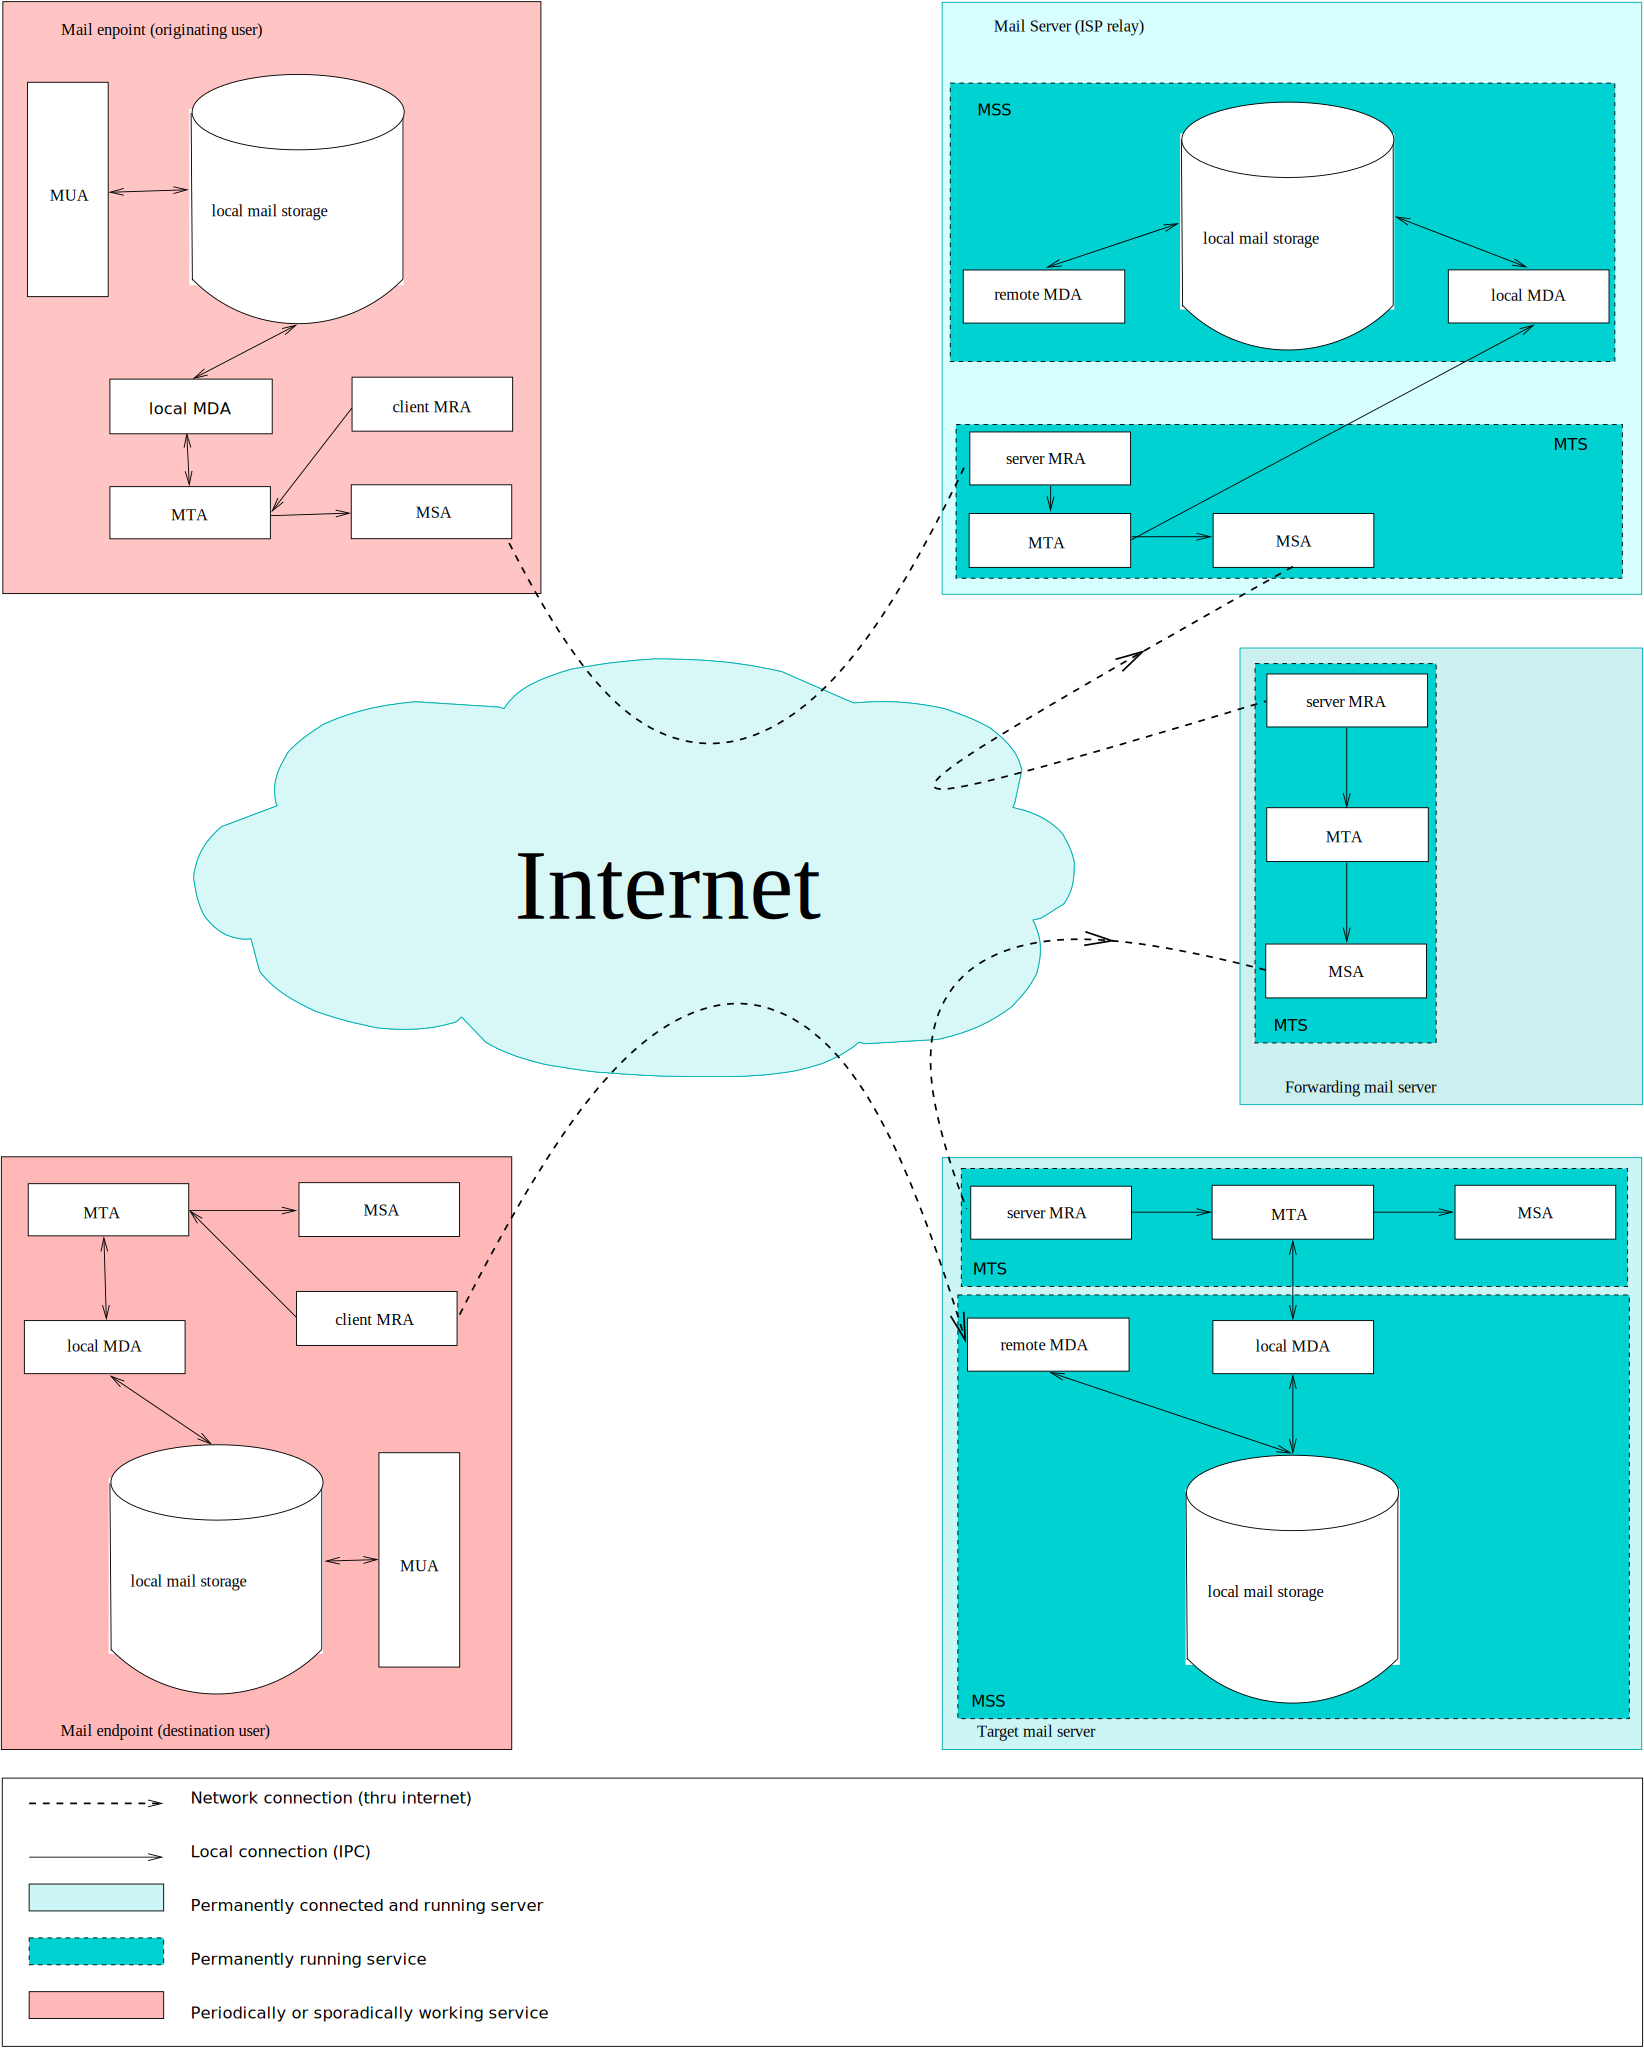
\includegraphics[width=\columnwidth]{inc/MailAgents1.pdf}
	\caption{Mail Agents}\label{fig:MailAgents}
\end{figure}

In the following paragraphs (for definitions), the term ``email'' is used synonymously to the term ``Message''.  ``Email'' has been chosen over ``messages'' because of its frequent use in standard documents.

Emails are typically initiated by a Mail User Agent (\defref{MUA}). An MUA accesses local email storage, which may be the server storage or a local copy. The local copy may be a cache only copy, the only existing storage (when emails are fetched and deleted from the server after retrieval), or a collected representation of multiple server storages (cache or authoritative).

Besides the MUA, the only other component accessing local email storage is the Mail Delivery Agent (\defref{MDA}). An MDA is responsible for storing and fetching emails from the local mail storage. Emails destined for other accounts than the current one are forwarded to the MTA. Emails destined to a User are persistently stored in the local email storage. It is essential to understand that email storage does not necessarily reflect a single mailbox. It may as well represent multiple mailboxes (e.g., a rich client-serving multiple IMAP accounts) or a combined view of multiple accounts (e.g., a rich client collecting mail from multiple \defref{POP} accounts). In the case of a rich client, the local MDA is part of the software provided by the user agent. In the case of an email server, the local MDA is part of the local email store (not necessarily of the mail transport service).

On the server-side, there are usually two components (services) at work. A ``Mail Transport Service'' (\defref{MTS}) responsible for mail transfers and a ``Mail Storage System'' which offers the possibility to store received Mails in a local, persistent store.\par

An MTS generally consists out of three parts. For incoming connects, there is a daemon called Mail Receiving Agent (\defref{Server MRA}) is typically a \defref{SMTP} listening daemon. A Mail Transfer Agent (\defref{MTA}) which is responsible for routing, forwarding, and rewriting emails. Moreover, a Mail Sending Agent (\defref{MSA}) which is responsible for transmitting emails reliably to another Server MRA (usually sent via \defref{SMTP}).\par

An MSS consists of local storage and delivery agents which do offer uniform interfaces to access the local store. They do also deal with replication issues, and grant should take care of the atomicity of transactions committed to the storage. Typically there are two different kinds of \defref{MDA}s. \defref{Local MDA}s offer possibilities to access the store via efficient (non-network based) mechanisms (e.g., IPC or named sockets). This is usually done with a stripped-down protocol (e.g., \defref{LMTP}). For remote agents there a publicly -- network-based -- agent available. Common Protocols for this \defref{Remote MDA}\ include \defref{POP}, \defref{IMAP}, or \defref{MS-OXCMAPIHTTP}.\par

Mail endpoints consist typically of the following components:
\begin{itemize}
	\item A Mail User agent (\defref{MUA})
	\item A Local Mail storage (\defref{MUA})
	\item A Local Mail Delivery Agent (\defref{Local MDA})
	\item A Mail Transfer Agent (\defref{MTA})
	\item A Mail Sending Agent (\defref{MSA})
	\item A Mail Receiving Agent (\defref{MRA})
\end{itemize}

Only two of these components do have external interfaces. These are \defref{MSA} and \defref{MRA}. \defref{MSA} usually uses \defref{SMTP} as transport protocol. When doing so, there are a couple of specialties. 
\begin{itemize}
	\item Port number is 587 (specified in \cite{RFC4409}).\\
	Although port numbers 25 and 465 are valid and do usually have the same capabilities, they are for mail routing between servers only. Mail endpoints should no longer use them.
	\item Connections are authenticated.\\
	Unlike a normal server-to-server (relay or final delivery) SMTP connections on port 25, clients should always be authenticated of some sort. This may be based on data provided by the user (e.g., username/password or certificate) or data identifying the sending system (e.g., IP address)\cite{RFC4409}. Failure in doing authentication may result in this port being misused as a sender for \defref{UBM}.
\end{itemize}

Mail User Agents (MUA) are the terminal endpoint of email delivery. Mail user agents may be implemented as fat clients on a desktop or mobile system or as an interface over a different generic protocol such as HTTP (Web Clients). 

Server located clients are a special breed of fat clients. These clients share the properties of fat clients except for the fact that they do not connect to the server. The client application itself has to be run on the server where the mail storage persists. This makes delivery and communication with the server different. Instead of interfacing with an MSA and a client MDA, they may directly access the local mail storage on the server. On these systems, the local mail storage may be implemented as a database in a user-specific directory structure.

\subsubsection{Fat clients}
The majority of mail clients are fat clients. These clients score over the more centralistic organized web clients in the way that they may offer mail availability even if an Internet connection is not available (through client-specific local mail storage). They furthermore provide the possibility to collect emails from multiple sources and store them in the local storage. Unlike Mail servers, clients are assumed to be not always online. They may be offline most of the time. To guarantee the availability of a particular email address, a responsible mail server for a specific address collects all emails (the \defref{MSS} does this) and provides a consolidated view onto the database when a client connects through a local or remote MDA.

As these clients vary heavily, it is mandatory for the MDA that they are well specified. Lack of doing so would result in massive interoperability problems. Most commonly the Protocols \defref{IMAP}, \defref{POP} and \defref{EWS} are being used these days. For email delivery, the SMTP protocol is used. 

Fat clients are commonly used on mobile devices. According to  \cite{clientDistribution} in Aug 2012 the most typical fat email client was Apple Mail client on iOS devices ($35.6\%$), followed by Outlook ($20.14\%$), and Apple Mail ($11\%$). \citetitle{clientDistribution2}\cite{clientDistribution2} as a more recent source lists in February 2014 iOS devices with $37\%$, followed by Outlook ($13\%$), and  Google Android ($9\%$).

\subsubsection{Server located clients}
Server located clients build an absolute minority. This kind of clients was common in the days of centralized hosts. An example for a Server Located Client is the Unix command ``mail''. This client reads email storage from a file in the users home directory.

\subsubsection{Web clients}
Web clients are these days a common alternative to fat clients. Most big provider companies use their proprietary web client. According to \cite{clientDistribution2} the most common web clients are "`Gmail"', "`Outlook.com"', and "`Yahoo! Mail"'. All these Interfaces do not offer a kind of public plug-in interface. However,  they do offer IMAP-interfaces. This important for a future generalistic approach to the problem.

\section{S/MIME (1996)}
S/MIME is an extension to the MIME standard. The MIME standard allows in simple text-oriented mails an alternate representation of the same content (e.g., as text and as HTML), or it allows to split a message into multiple parts that may be encoded. It is important to note that MIME encoding is only effective in the body part of a mail.

S/MIME, as described in \cite{RFC3851}, extends this standard with the possibility to encrypt mail content or to sign it. Practically this is achieved by either putting the encrypted part or the signature into an attachment. It is essential to know that this method leaks significant pieces of the data.

As the mail travels directly from sender to recipient, both involved parties are revealed. Neither message subject nor message size or frequency is hidden. This method does offer limited protection when assuming an adversary with interest in the message content only. It does not protect from the kind of adversary in our case. 

The trust model is based on a centralistic approach involving generally trusted root certification authorities.

\section{Pretty Good Privacy (1996)}
Exactly as S/MIME PGP\cite{rfc4880} builds upon the base of MIME. Although the trust model in PGP is peer-based. The encryption technology does not significantly differ (as seen from the security model).

Like S/MIME, PGP does not offer anonymity. Sender and endpoints are known to all routing nodes. Depending on the version of PGP, some meta-information or parts of the message content such as subject line, the real name of the sender and receiver, message size is leaked.

A good thing to learn from PGP is that peer-based approaches are offering limited possibilities for trust. The trust in PGP is based on the peer review of users. This peer review may give an idea of how well verified the key of a user is.


\chapter{Information Routing and Distribution for Anonymizing Protocols}
\fxwarning{complete section}

\section{Mixing}
Mixes have been first introduced by \citetitle{CHAUM1}\cite{CHAUM1} in \citeyear{CHAUM1}. The basic concept in a mix goes as follows. We do not send a message directly from the source to the target. Instead, we use a kind of proxy server or router in between which picks up the packet, anonymizes it, and forwards it either to the recipient or another mix. If we assume that we have at least three mixes cascaded, we then can conclude that:
\begin{itemize}
	\item Only the first mix knows the true sender
	\item All intermediate mixes know neither the true sender nor the true recipient (as the data comes from mixes and is forwarded to other mixes) 
	\item Only the last mix knows the final recipient.
\end{itemize}

This approach (in this simple form) has several downsides and weaknesses.

\begin{itemize}
	\item In a low latency network, the message may be traced by analyzing the timing of a message.
	\item We can emphasize a path by replaying the same message multiple times (assuming we control an evil node), thus discovering at least the final recipient.
	\item If we can ``tag'' a message (with content or attribute), we then may be able to follow the message.
\end{itemize}

In \citeyear{RP03-1} \citeauthor{RP03-1} analyzed the suitability for mixes as an anonymizing network for masses. They concluded that there are three possibilities to run mixes.
\begin{itemize}
	\item Commercial, static MixNetworks
	\item Static MixNetworks operated by volunteers
	\item Dynamic MixNetworks
\end{itemize}
They concluded that in an ideal implementation, a dynamic mix network where every user is operating a mix is the most promising solution as static mixes always might be hunted by an adversary.

\section{Anonymous Remailers}
Remailers have been in use for quite some time. There are several classes of remailers, and all of them are somehow related to Mixnets. There are ``types'' of remailers defined. Although these ``types'' offer some hierarchy, none of the more advanced ``types'' seem to have more than one implementation in the wild. 

Pseudonymous Remailers (also called Nym Servers) take a message and replace all information pointing to the original sender with a pseudonym. This pseudonym may be used as an answer address. The most well known pseudonymous remailer possibly was anon.penet.fi run by Johan Helsingius. This service has been forced several times to reveal a pseudonyms true identity before Johan Heösingius decided to shut it down. For a more in-depth discussion of Pseudonymous Remailers see \ref{sec:remPseudo}

Cypherpunk remailers forward messages like pseudonymous remailers. Unlike pseudonymous remailers, Cypherpunk remailers decrypt a received message, and its content is forwarded without adding a pseudonym. A reply to such a message is not possible. They may, therefore, be regarded as an ``decrypting reflector'' or a ``decrypting mix'' and may be used to build an onion routing network for messages. For a more in-depth discussion of type-1-remailers, see section  \ref{sec:remCypherpunk}.

Mixmaster remailers are very similar to Cypherpunk remailers. Unlike them, Mixmaster remailers hide the messages, not in an own protocol, but use \defref{SMTP} instead. While using \defref{SMTP} as a transport layer, Cypherpunk remailers are custom (non-traditional mail) servers listening on port 25. For a more in-depth discussion of type-2-remailers, see section \ref{sec:remMixmaster}.

Mixminion remailers extend the model of Mixmaster remailers. They still use \defref{SMTP} but introduce new concepts. New concepts in Mixminion remailers are:
\begin{itemize}
	\item Single Use Reply Blocks (SURBs)
	\item Replay prevention
	\item Key rotation
	\item Exit poicies
	\item Dummy traffic
\end{itemize}
For a more in depth discussion of Mixminion remailers see section \ref{sec:remMixminion}.


\section{Onionizing}
Onion routing is a further development of the concept of mixes. In onion routers, every mix gets a message which is asymmetrically encrypted. By decrypting the message, he gets the name of the next-hop and the content which he has to forward. The main difference in this approach is that in traditional mix cascades, the mix decides about the next hop. In an onionised routing system, the message decides about the route it is taking. 

While tagging attacks are far harder (if we exclude side-channel attacks to break sender anonymity), the traditional attacks on mixes are still possible. So when an adversary is operating entry and exit nodes, it is straightforward for them to match the respective traffic.

One very well known onion routing network is Tor (\href{https://www.torproject.org}{https://www.torproject.org}). For more information about Tor see section \ref{sec:tor}.

\section{Crowds}
Crowds is a network that offers anonymity within a local group. It works as follows:

\begin{itemize}
	\item All users add themselves to a group by registering on a so-called ``blender''.
	\item All users start a service (called JonDo).
	\item Every JonDo takes any received message (might be from him as well) and sends it with a 50\% chance either to the correct recipient or to a randomly chosen destination
\end{itemize}

While crowds as specified in \cite{crowds:tissec} does anonymize the sender from the recipient rather well, the system offers no protection from someone capable of monitoring crowds traffic. The system may, however, be easily attacked from within by introducing collaborating johndos. It has been further developed to D-Crowds \cite{DBLP:conf/esorics/DanezisDKT09}, ADU/RADU \cite{Munoz-Gea2008}, Freenet\cite{freenet} and others. 

Furthermore, the blender is aware of all JonDos and thus of particular interest for any observing or censoring adversary. Control of the blender enables an adversary to split the network into controllable parts, adding a high likelihood of discovering an original sender.

\section{Mimic Routes}
Mimics are a set of statical mixes which maintain a constant message flow between the static routes. If legitimate traffic arrives, the pseudo traffic is replaced by legitimate traffic. An outstanding observer is thus incapable of telling the difference between real traffic and dummy traffic.

If centralized mixes are used, the system lacks the same vulnerabilities of sizing and observing the exit nodes as all previously mentioned systems. If we assume that the sender and receiver operate a mixer by themselves, the system would no longer be susceptible to timing or sizing analyses. The mimic routes put a constant load onto the network. This bandwidth is lost and may not be reclaimed. It does not scale well as every new participant increases the need for mimic routes and creates (in the case of user mixes) a new mimic load. Furthermore, the mixes are easily identifiable as their characteristic data stream contrasts compared to other network service streams.

\section{Distributed Hash Tables}
\fxwarning{complete section}

\section{Dining Cryptographer Networks}
DC networks are based on the work \citetitle{chaum-dc} by \citeauthor{chaum-dc}\cite{chaum-dc}. In this work, \citeauthor{chaum-dc} describes a system allowing a one-bit transfer (The specific paper talks about the payment of a meal). Although all participants of the DC net are known, the system makes it unable to determine who has been sending a message. The message in a DC-Net is readable for anyone. This network has the downside that a cheating player may disrupt communication without being traceable.

Several attempts have been made to strengthen the proposal of Chaum\cite{golle:eurocrypt2004,disco,herbivore:tr,Corrigan-Gibbs:2010:DAA:1866307.1866346}. However, no one succeeded without introducing significant downsides on the privacy side.

\chapter{Proposed Academic Protocols and System Implementations}
\fxwarning{complete section}
\section{Characteristics of Known Anonymity Implementations}
Table \ref{tab:anonClass} shows the previously analyzed protocols.

\begin{table*}[t]\centering\tiny
	\label{tab:anonClass}
	\setlength{\aboverulesep}{0pt}
	\setlength{\belowrulesep}{0pt}
	\newcolumntype{x}[1]{!{\centering\arraybackslash\vrule width #1}}
	% network
	%\usepackage{ amssymb }
	\newcommand\fullyn{$\boxtimes$}
	\newcommand\mostlyn{$\square$}
	\newcommand\partlyn{$\sqsubset$}
	%direction
	\newcommand\bidi{$\longleftrightarrow$}
	\newcommand\unidi{$\longrightarrow$}
	% synchronization
	\newcommand\async{$\neq$}
	\newcommand\sync{$\cong$}
	% symmetry
	\newcommand\ptp{\scalebox{0.4}{$\bullet\cdots\bullet\cdots\bullet$}}
	\newcommand\cs{\scalebox{0.4}{$\bullet\cdots\bullet$}}
	\newcommand\hybrid{\scalebox{0.4}{$\bullet\cdots\circ\cdots\bullet$}}
	% Hierarchy
	\newcommand\flath{$\cdots$}
	\newcommand\hierarch{\ding{68}}
	% centralization
	\newcommand\partcentr{\astrosun}
	\newcommand\decentr{$\circ$}
	% Network view
	\newcommand\fullynv{$\CIRCLE$}
	\newcommand\partlynv{$\LEFTcircle$}
	% NW updating
	\newcommand\timed{\clock}
	\newcommand\event{\lightning}
	\newcommand\noupd{\ding{56}}
	% Routing
	\newcommand\routesrc{\scalebox{0.4}{$\bullet\cdots$}}
	\newcommand\routehop{\scalebox{0.4}{$\cdots\bullet\cdots$}}
	\newcommand\routebc{\faBullhorn}
	% Routing
	\newcommand\shedfair{$\equiv$}
	\newcommand\shedprio{$\Diamonddot$}
	%determinism
	\newcommand\nsdetdet{\checkmark}
	\newcommand\nsdetprob{$\ding{56}$}
	%determinism
	\newcommand\nsnodesall{\CircledA}
	\newcommand\nsnodessec{\Stopsign}
	\newcommand\nsnodesnet{\Mundus}
	\newcommand\nsnodesusr{\smiley}
	% probability
	\newcommand\nsprobuni{$\circledast$}
	\newcommand\nsprobstat{$\circledcirc$}
	\newcommand\nsprobdyn{$\ast$}
	% latency
	\newcommand\perflatl{L}
	\newcommand\perflath{H}
	\newcommand\perflatm{M}
	% mode 
	\newcommand\perfmodecon{$\multimapdotboth$}
	\newcommand\perfmodemsg{$\Letter$}
	% implementation
	\newcommand\nsimplyes{\checkmark}
	\newcommand\nsimplno{$\ding{56}$}
	% code available
	\newcommand\nscodeyes{\checkmark}
	\newcommand\nscodeno{$\ding{56}$}
	% context
	\newcommand\nscontmsg{\faEnvelope}
	\newcommand\nscontmail{@}
	\newcommand\nscontbulletin{\faUsers}
	\newcommand\nscontphone{\Telefon}
	\newcommand\nscontwww{\faInternetExplorer}
	\newcommand\nscontmicroblog\faPencil
	\newcommand\nscontfiles\faStickyNote
	\newcommand\nscontwifi\faWifi
	\gdef\cwidth{0.37cm}
	\rowcolors{8}{black!30}{black!10}
	\begin{tabular}{x{2pt}lx{2pt}*{5}{p{\cwidth}|}p{\cwidth}x{2pt}p{\cwidth}|p{\cwidth}x{2pt}*{4}{p{\cwidth}|}p{\cwidth}x{2pt}*{4}{p{\cwidth}|}p{\cwidth}x{2pt}}
		\toprule
		
		& \multicolumn{6}{cx{2pt}}{Network Structure} & \multicolumn{2}{p{1.2cm}x{2pt}}{\centering Routing Information} & \multicolumn{5}{cx{2pt}}{Communication Model} & \multicolumn{5}{cx{2pt}}{Performance and Deployability}\\\cmidrule{2-19}
		
		& & \multicolumn{2}{c|}{Connection} & \multicolumn{3}{cx{2pt}}{Symmetry} & & & & & \multicolumn{3}{cx{2pt}}{Node Selection} & & & & & \\\cmidrule{3-4}\cmidrule{5-7}\cmidrule{12-14}
		
		& \rot{Topology} & \rot{Direction} & \rot{Synchronization} & \rot{Roles} & \rot{Hierarchy} & \rot{Decentralization} & \rot{Network view} & \rot{Updating} & \rot{Routing Type} & \rot{Scheduling} & \rot{Determinism} & \rot{Selection set} & \rot{selection probability} & \rot{Latency} & \rot{Communication mode} & \rot{Implementation} & \rot{Code availability} & \rot{Context/application} \\
		\midrule
		MessageVortex & \fullyn & \bidi & \async & \ptp & \flath & \decentr & \partlynv &  \event &  \routesrc & \shedfair & \nsdetprob & \nsnodesusr & \nsprobuni & \perflath & \perfmodemsg & \nsimplyes & \nscodeyes & \nscontmail \\
		Riffle & & & & & & & & & & & & & & & & & & \\
		Atom & & & & & & & & & & & & & & & & & & \\
		Riposte & & & & & & & & & & & & & & & & & & \\
		Pung & & & & & & & & & & & & & & & & & & \\
		PIR & & & & & & & & & & & & & & & & & & \\
		Karaoke & & & & & & & & & & & & & & & & & & \\
		Loopix & & & & & & & & & & & & & & & & & & \\
		Stadium & & & & & & & & & & & & & & & & & & \\
		Vuvuzela & & & & & & & & & & & & & & & & & & \\
		\bottomrule
	\end{tabular}
	\caption{Classification table for anonymization protocols according to \cite{Shirazi2018}}
\end{table*}
\section{Resenders, Onion Routers, and MixNets}
\subsection{Pseudonymous Remailers (1981)\label{sec:remPseudo}}
\fxwarning{Section missing}

\subsection{Cypherpunk Remailers (approx. 1993)\label{sec:remCypherpunk}}
With the failing of anon.penet.fi, it became clear that the weakest spot of a single server infrastructure the information stored on the server and the vulnerability of their owner. The new type-1-remailers score over the existing type-0-remailers by using encryption for the message. Most of the time PGP was used and custom programmed mail processors on systems to achieve the functionallity. It is unclear when first type-1-remailers were invented. Setting up a type-1-remailer was typically achieved by using procmail together with a small script calling PGP binaries and then sending the resulting message to the next recipient. By combining multiple type-1-remailers, an onion-like structure of the message was achievable. 

This approach was promising, but it was still observable. An observation was possible by correlating the message sizes (e.g., strictly decreasing) and timing information. Furthermore, remailers were however still known and authorities were able to ban infrastructure and capable of monitoring their routing activities. Additionally, those remailers allowed to prosecute administrators of such systems.

\subsection{Babel (1996)}
Babel was an academic system defined in a paper by \citeauthor{babel} in \citeyear{babel}\cite{babel}. It has been developed at IBM Zurich Research Laboratory. It was a mixing system using onionized addresses. The sender remains anonymous while he may provide a reply routing block called RPI. If both parties would like to remain anonymous, the RPI of the initiator is deployed in a forum thread. Anyone using this block adds an RPI for its address to the message.

This system has all the disadvantages of a system using MURBs. Traffic highlighting and similar attacks are possible.

\subsection{Mixmaster-Remailers (1996)\label{sec:remMixmaster}}
Like Cypherpunk remailers, the Mixmaster remailers were working with onion-like encrypted messages. The protocol was based on Mix-Nets described by Chaum in \cite{CHAUM1} and further developed by L. Cotrell in 1996. 

In contrast to type-1-remailers, the use of cascading systems to remail became systematic. The enduser used specialized software to build and send Mixmaster messages.

Mixmaster messages were still traceable by message size. Reply blocks were not supported by the system. A user had to know all Mixmaster nodes in order to use the system. The last node was typically an exit node sending the message in clear to the final recipient. This behavior still allowed the use of Usenet.

\subsection{Crowds (1997)}

\fxwarning{Add section}


\subsection{Tor (2000)\label{sec:tor}}
Tor is one of the most common onion router networks these days and onionizes generic TCP streams. It is specified in \cite{tor-spec}. It might be considered one of the most advanced networks since it has a considerable size, and much research has been done here.

According to \cite{onion-routing:pet2000} Tor is a network consisting of multiple onion routers. Each client first picks an entry node. Then it establishes an identity, gets a listing of relay servers, and chooses a path through multiple onion routers. The temporary identity links to such a path and should be changed on a regular base along with its identity. Transferring data works by splitting the data into equally sized cells of 512 bytes.

There is a centrally organized directory in the Tor network, knowing all tor relay servers. Any Tor relay server may be a directory server as well. 

Many attacks involving the Tor networks have been discussed in the academic world such as \cite{hs-attack06,esorics13-cellflood,bauer:wpes2007,esorics12-torscan,oakland2013-trawling,danner-et-al:tissec12,congestion-longpaths} and some have even been exploited actively. In the best case, the people discovering the attacks did propose mitigation to the attack. Some of these mitigations flowed back into the protocol. Some general thoughts of the attacks should be emphasized here for treatment in our protocol.

Being an exit node may be a problem in some jurisdictions. In general, it seems to be accepted that routing traffic with unknown content (to the routing node) is not regarded as illegal per se. So by being unable to tell malicious or illegal traffic apart from legitimate traffic, this is not a problem. However -- being an exit node can mean that unencrypted and illegal traffic is leaving the routing traffic. In this specific case, operators of a relay node might fear legal prosecution. Tor nodes may proclaim themselves as  `` non-exit nodes''  to avoid the possibility of legal prosecution.

Furthermore, several DoS-Attacks have been carried out to overload parts of the Tor network. Most of them do a bandwidth drain on the network layer.

Attacking anonymization has been done in several ways. First of all, the most common attack is a time-wise correlation of packets if in control of an entry and an exit node. A massive attack of this kind was published in 2014 and has been published on the tor website (\href{https://blog.torproject.org/blog/tor-security-advisory-relay-early-traffic-confirmation-attack}{relay early traffic confirmation attack}). This attack was possible because tor is a low latency network. Another attack is to identify routes through tor by statistically analyze the traffic density in the network between nodes. More theoretical attacks focus on the possibility of controlling the directory servers to guarantee that an entity may be deanonymized because it is using compromised routers.

Generally, the effectiveness of the monitoring of single nodes or whole networks is disputed. According to a study by \citeauthor{ccs2013-usersrouted} in \citeyear{ccs2013-usersrouted}\cite{ccs2013-usersrouted}, a system in the scale of PRISM should be able to correlate traffic of 95\% of the users within a ``few days''. Other sources based on the Snowden Papers claim that NSA was unable so far to de-anonymize users of  Tor. However, since these papers referenced to ``manual analysis'', the statement may be disputed when looking at automated attacks as well.

It is, according to \url{https://www.torproject.org/docs/pluggable-transports}, impossible to use transborder Tor traffic in at least China, Uzbekistan, Iran, and Kazakstan. In censored countries, Tor offers so-called bridged Transports. Currently deployed transports in the standard Tor browser bundle package are obfs4, meek, FTE, and ScrambleSuit. Only meek is listed as working in China. Meek achieves this by hiding its traffic in a standard protocol (https).

\cite{saleh2018shedding} is an excellent survey listing recent developments and attacks within the Tor project.

\subsection{\texorpdfstring{$I^2P$}{I2P} (2001)}
The name $I^2P$ is a derived from  ``Invisible Internet Project'' according to \href{https://geti2p.net/}{geti2p.net}. The first binary relase on sourceforge dates from 2001. The system itself is comparable to Tor for its capabilities. Mayor differences are:
\begin{itemize}
	\item P2P based
	\item Packet-switched routing (tor is ``circuit-switched'')
	\item Different forward and backward routes (called tunnels)
	\item Works pseudonymously
	\item Supports TCP and UDP
\end{itemize}

$I^2P$ has not attracted as much attention as Tor so far. So it is hard to judge upon its real qualities.

In \citeyear{pets2011-i2p} \citeauthor{pets2011-i2p} presented in \cite{pets2011-i2p} an attack. As $I^2P$s security model is chosen based on IP addresses, the authors propose to use several cloud providers in different B-Class networks. By selectively flooding peers, an adversary may extract statistical information. The paper proposes an attack based on the heuristic performance-based peer selection. The main critics of the paper were that the peer selection might be influenced by an adversary enabling him to recover $I^2P$ has not attracted as much attention as Tor so far. So it is hard to judge upon its real qualities.

In \citeyear{pets2011-i2p} \citeauthor{pets2011-i2p} presented in \cite{pets2011-i2p} an attack. As $I^2P$s security model is chosen based on IP addresses, the authors propose to use several cloud providers in different B-Class networks. By selectively flooding peers, an adversary may extract statistical information. The paper proposes an attack based on the heuristic performance-based peer selection. The main critics of the paper were that the peer selection might be influenced by an adversary enabling him to recover data on a statistical base.

\subsection{Mixminion-Remailers (2002)\label{sec:remMixminion}}
Mixminion was the standard implementation of a type-3-remailer. It tried to address many issues previously not solved. A Mixminion router splits messages in equally sized chunks and supports SURBs. Furthermore,  replay protection and key rotation were available. Unlike the previous remailer types, Mixminion was no longer using \defref{SMTP} as the transport protocol. Instead, Mixminion introduced a new transport protocol. The sources of this remailer are available on GitHub under https://github.com/mixminion/mixminion.

As a received message had to be decoded by the final recipient. Therefore, the final recipient had to be aware of Mixminion system.

According to \url{https://mixminion.net} the first release of the software was in December 2002. And has been discontinued in 2008. Since 2011 the sources are available on GitHub. Therehave been some forks in 2011 but at the moment all forks seem to be inactive since at least 2016 as there are no new commits.

\subsection{\texorpdfstring{$\mathcal{P}^5$}{P5} (2002)}
The Peer-to-Peer Personal Privacy Protocol is defined in \cite{sherwood-protocol}. It provides sender-, receiver- and sender-receiver anonymity. According to the project page of $\mathcal{P}^5$, there is only a simulator available for the protocol.

The transport layer problematic has been wholly ignored. As there is no precise protocol specification but only a rough outline about the messaging and the crypto operations, $\mathcal{P}^5$ offers minimal possibilities for analysis.

\subsection{AN.ON (2003)}
AN.ON, as suggested in \cite{federrath2003system}, is a mixing network. It generates messages in equally sized chunks and sends them in fixed time slots after random mixing. Its implementation is called JAP and may be found under https://anon.inf.tu-dresden.de/. JAP is many ways similar to the capabilities of Tor. The network was at the time of writing a lot smaller (10 JonDos compared to 6500 relays in the Tor network).

While the approach is both simple and effective, it is not suitable against a powerful adversary. First, an adversary may be able{\tiny } to snoop the forwarding when on the system. Second, due to the timing behavior, tunnels belonging to each other may be identified, and third, the package size information does leak as well.


\subsection{AP3 (2004)}
AP3, as defined in \cite{mislove2004ap3}, is an anonymous communication system and very similar to crowds. It performs a random walk over a set of known nodes. Not all nodes are known to anyone, and all nodes are aware of the final recipient. 

The system is susceptible to numerous attacks, as shown by \cite{ccs2008:mittal}, and does not withstand our adversary as the final recipient is known to the routing nodes.

\subsection{Cashmere (2005)}
Cashmere is specified in \cite{zhuang2005cashmere}. It defines a protocol for the use of chaum mixes. Unlike most of the protocols, the chaum mixes in cashmere are virtual. So-called relay groups represent them. Each mix in the relay group may be used as an equivalent mix to all other mixes in the same group. 

This design means that the failure of one mix does not result in the non-delivery of a message.

No client implementation could be found on the \textit{}nternet. The project homepage \href{http://current.cs.ucsb.edu/projects/cashmere/}{http://current.cs.ucsb.edu/projects/cashmere/} has not been updated since 2005. This suggests that this project is dead or sleeping.

\subsection{SOR (2012)}
SSH-based onion routing (SOR)\cite{Egners_2012} is blaming the complex and monocultural landscape of anonymizing software and proclaims a simple approach based on onionized SSH tunnels. 

\subsection{SCION (2017)}
SCION\cite{perrig2017scion} is a clean slate Internet protocol. While SCION is not really an anonymizing protocol. It contains, however,  many interesting features. Unlike with the traditional networks, we have the possibility of influencing the routing of data within SCION. Furthermore, with PHI\cite{chen2017phi} and Dovetail\cite{sankey2014dovetail}, SCION may feature strong and fast anonymity features. 

Unfortunately, as this is a clean slate Internet design, it is not available commonly currently, and as it is easily identifiable, it enables easy censorship as the relevance is due to its current availability of no importance, and a censoring adversary may just ban and censor SCION entirely. 

\section{Distributed Hash Tables}
\subsection{Tarzan (2002)}
Tarzan is a P2P IP protocol using UDP to communicate. It is specified in \cite{tarzan:ccs02}. Tarzan nodes may be used to anonymize Internet traffic in general. An initiator on the original sender machines encapsulates traffic into a layered UDP package and sends the package through a mix like relayd's. The last relayd acts as an exit node. A replier may send answers the opposite way. Each relayd knows its next and previous relayd. To minimize the impact of observation, Tarzan forwards packets only every 20ms and features replay protection.

\subsection{MorphMix (2002)}
MorphMix is another mix network and specified in \cite{morphmix:wpes2002}. It was a circuit-based mix system for networking anonymity. The core of the network was collision detection. This detection has been circumvented by \cite{morphmix:pet2006}. Since then, no new papers have been published, and the project seems to be dead.

\subsection{Salsa (2008)}
Salsa was proposed in \cite{Salsa} and described a circuit based anonymization pattern based on distributed hash tables (DHT). An implementation for Salsa is available, but it is not public. \cite{ccs2008:mittal} claims that by combining active and passive attacks, anonymity can be compromised.

\section{Dining Cryptographer Based Network}
\subsection{Herbivore (2003)}
Herbivore is a network protocol designed by \citeauthor{herbivore:tr} in \cite{herbivore:tr}. It is based on the dining cryptographers paper\cite{chaum-dc}. At the time of writing, no herbivore client or an actual protocol implementation could be found on the Internet. Wikipedia lists Herbivore as ``dormant or defunct''.

\subsection{Dissent (2010)}
Dissent is defined in \cite{Corrigan-Gibbs:2010:DAA:1866307.1866346}. It is an anonymity network based on DC-nets. A set of servers forms these DC-nets. At least one of the servers in the used net must be trustworthy, and none may be misbehaving. A server failure results in the stall of all message delivery using this server.

\section{Broadcast and Multicast Networks}
\subsection{Hordes (2002)}
Hordes was a multicast-based protocol for anonymity specified in \cite{Levine:2002}. Hordes used the abilities to handle multicast addresses of routers to generate a dynamic set of receivers and then sends messages to them. It assumes that a single observer or router does not know all participating peers. 


This assumption is correct for a local observer. Unfortunately, it is not sufficient assuming an adversary as defined in this paper.

\section{Distributed Storage Systems}
\subsection{Feenet (2000)}
Freenet was initially designed to be a fully distributed data store\cite{freenet}. Documents are stored in an encrypted form. Downloaders must know a document descriptor called CHK containing the file hash, the key, and some background about the crypto being used. A file is stored more or less redundantly based on the number of accesses to a stored file. The primary goal of Freenet is to decouple authorship from a particular document. It furthermore provides fault-tolerant storage, which improves caching of a document if requested more often.

Precisely as $I^2P$, Freenet is not analyzed thoroughly by the scientific world. 

The Freenet features two protocols FCPv2 acts as the client protocol for participating in the control of the Freenet storage. The Freenet client protocol allows us to insert and retrieve data, to query the network status, and to manage Freenet nodes directly connected to an own node. FCPv2 operates on port 9481, and blocking is thus easy, as it is a dedicated port. 

The Freenet project seems to be under active development as pages about protocols were updated in the near past (Last update on the FCPv2 Page was July \nth{5} 2016 at the time of writing).

\subsection{Gnutella (2000)}
Gnutella is not a protocol for the anonymity world in special. Instead, the Gnutella protocol implements a general file sharing on a Peer to peer base. This peer-to-peer approach is the most interesting aspect of Gnutella in this context. Furthermore, Gnutella has proven to be working with a large number of clients.

The current protocol specification may be found under \href{http://rfc-gnutella.sourceforge.net/developer/stable/index.html}{http://rfc-gnutella.sourceforge.net/}. While the Gnutella network is defunct. The approaches solving some of the peer-to-peer aspects were very interesting.

\subsection{Gnutella2 (2002)}
Despite its name, Gnutella2 is not the next generation of Gnutella. It was a fork in 2002 from the original Gnutella and has been developed in a different direction. The specification may be found on \url{http://g2.doxu.org}. Just as its predecessor, Gnutella2 seems to be dead. The last relevant update to the main site or its protocol is dated four years back.

\section{Unknown (TBD)}
\subsection{Riffle (2016)}
\cite{kwon2016riffle}

\fxwarning{Add Riffle}%

\subsection{Atom (2016)}
\cite{kwon2016atom}

\fxwarning{Add Atom}%

\subsection{Riposte (2015)}
\cite{corrigan2015riposte}

\fxwarning{Add Riposte}%

\subsection{Pung (2016)}
\cite{angel2016unobservable}

\fxwarning{Add Pung}%

\subsection{PIR (2018)}
\cite{angel2018pir}

\fxwarning{Check PIR}%

\subsection{Karaoke (2018)}
\cite{lazar2018karaoke}

\fxwarning{Add Karaoke}%

\subsection{Loopix (2017)}
\cite{piotrowska2017loopix}

\fxwarning{Add Loopix}%

\subsection{Stadium (2017)}
\cite{tyagi2017stadium}

\fxwarning{Add Stadium}%

\subsection{Vuvuzela (2015)}
\cite{van2015vuvuzela}

\fxwarning{Add Vuvuzela}%



%%%% REMOVE HERE


\subsection{Characteristics of known anonymity Systems}
Table \ref{tab:anonClass} shows the previously analyzed protocols.

\begin{table*}[t]\centering\tiny
	\label{tab:anonClass}
	\setlength{\aboverulesep}{0pt}
	\setlength{\belowrulesep}{0pt}
	\newcolumntype{x}[1]{!{\centering\arraybackslash\vrule width #1}}
	% network
	%\usepackage{ amssymb }
	\newcommand\fullyn{$\boxtimes$}
	\newcommand\mostlyn{$\square$}
	\newcommand\partlyn{$\sqsubset$}
	%direction
	\newcommand\bidi{$\longleftrightarrow$}
	\newcommand\unidi{$\longrightarrow$}
	% synchronization
	\newcommand\async{$\neq$}
	\newcommand\sync{$\cong$}
	% symmetry
	\newcommand\ptp{\scalebox{0.4}{$\bullet\cdots\bullet\cdots\bullet$}}
	\newcommand\cs{\scalebox{0.4}{$\bullet\cdots\bullet$}}
	\newcommand\hybrid{\scalebox{0.4}{$\bullet\cdots\circ\cdots\bullet$}}
	% Hierarchy
	\newcommand\flath{$\cdots$}
	\newcommand\hierarch{\ding{68}}
	% centralization
	\newcommand\partcentr{\astrosun}
	\newcommand\decentr{$\circ$}
	% Network view
	\newcommand\fullynv{$\CIRCLE$}
	\newcommand\partlynv{$\LEFTcircle$}
	% NW updating
	\newcommand\timed{\clock}
	\newcommand\event{\lightning}
	\newcommand\noupd{\ding{56}}
	% Routing
	\newcommand\routesrc{\scalebox{0.4}{$\bullet\cdots$}}
	\newcommand\routehop{\scalebox{0.4}{$\cdots\bullet\cdots$}}
	\newcommand\routebc{\faBullhorn}
	% Routing
	\newcommand\shedfair{$\equiv$}
	\newcommand\shedprio{$\Diamonddot$}
	%determinism
	\newcommand\nsdetdet{\checkmark}
	\newcommand\nsdetprob{$\ding{56}$}
	%determinism
	\newcommand\nsnodesall{\CircledA}
	\newcommand\nsnodessec{\Stopsign}
	\newcommand\nsnodesnet{\Mundus}
	\newcommand\nsnodesusr{\smiley}
	% probability
	\newcommand\nsprobuni{$\circledast$}
	\newcommand\nsprobstat{$\circledcirc$}
	\newcommand\nsprobdyn{$\ast$}
	% latency
	\newcommand\perflatl{L}
	\newcommand\perflath{H}
	\newcommand\perflatm{M}
	% mode 
	\newcommand\perfmodecon{$\multimapdotboth$}
	\newcommand\perfmodemsg{$\Letter$}
	% implementation
	\newcommand\nsimplyes{\checkmark}
	\newcommand\nsimplno{$\ding{56}$}
	% code available
	\newcommand\nscodeyes{\checkmark}
	\newcommand\nscodeno{$\ding{56}$}
	% context
	\newcommand\nscontmsg{\faEnvelope}
	\newcommand\nscontmail{@}
	\newcommand\nscontbulletin{\faUsers}
	\newcommand\nscontphone{\Telefon}
	\newcommand\nscontwww{\faInternetExplorer}
	\newcommand\nscontmicroblog\faPencil
	\newcommand\nscontfiles\faStickyNote
	\newcommand\nscontwifi\faWifi
	\gdef\cwidth{0.37cm}
	\rowcolors{8}{black!30}{black!10}
	\begin{tabular}{x{2pt}lx{2pt}*{5}{p{\cwidth}|}p{\cwidth}x{2pt}p{\cwidth}|p{\cwidth}x{2pt}*{4}{p{\cwidth}|}p{\cwidth}x{2pt}*{4}{p{\cwidth}|}p{\cwidth}x{2pt}}
		\toprule
		
		& \multicolumn{6}{cx{2pt}}{Network Structure} & \multicolumn{2}{p{1.2cm}x{2pt}}{\centering Routing Information} & \multicolumn{5}{cx{2pt}}{Communication Model} & \multicolumn{5}{cx{2pt}}{Performance and Deployability}\\\cmidrule{2-19}
		
		& & \multicolumn{2}{c|}{Connection} & \multicolumn{3}{cx{2pt}}{Symmetry} & & & & & \multicolumn{3}{cx{2pt}}{Node Selection} & & & & & \\\cmidrule{3-4}\cmidrule{5-7}\cmidrule{12-14}
		
		& \rot{Topology} & \rot{Direction} & \rot{Synchronization} & \rot{Roles} & \rot{Hierarchy} & \rot{Decentralization} & \rot{Network view} & \rot{Updating} & \rot{Routing Type} & \rot{Scheduling} & \rot{Determinism} & \rot{Selection set} & \rot{selection probability} & \rot{Latency} & \rot{Communication mode} & \rot{Implementation} & \rot{Code availability} & \rot{Context/application} \\
		\midrule
		MessageVortex & \fullyn & \bidi & \async & \ptp & \flath & \decentr & \partlynv &  \event &  \routesrc & \shedfair & \nsdetprob & \nsnodesusr & \nsprobuni & \perflath & \perfmodemsg & \nsimplyes & \nscodeyes & \nscontmail \\
		Riffle & & & & & & & & & & & & & & & & & & \\
		Atom & & & & & & & & & & & & & & & & & & \\
		Riposte & & & & & & & & & & & & & & & & & & \\
		Pung & & & & & & & & & & & & & & & & & & \\
		PIR & & & & & & & & & & & & & & & & & & \\
		Karaoke & & & & & & & & & & & & & & & & & & \\
		Loopix & & & & & & & & & & & & & & & & & & \\
		Stadium & & & & & & & & & & & & & & & & & & \\
		Vuvuzela & & & & & & & & & & & & & & & & & & \\
		\bottomrule
	\end{tabular}
	\caption{Classification table for anonymization protocols according to \cite{Shirazi2018}}
\end{table*}


\section{Pseudo Random Number Generators \label{sec:prng}}
The following sections list two PRNG specifications to follow the recommendations of \cite{rfc1750}. These PRNGs are used to complete the padding specified in the addRedundancy operation.

We have chosen to support two kinds of PRNG. These algorithms are not relevant for the security of the system, but they guarantee non-detectable padding when doing the addRedundancy operation. The two PRNGs selected were xorshift128+ and Blum Micail PRNG. Both PRNGs were quoted to pass BigCrush. However, recent development shows that this might not be true for xorshift128+, as demonstrated in \cite{LEMIRE2019139}.

\section{Known Attacks}
In the following sections, we emphasize on possible attacks to an anonymity preserving protocols. These attacks may be used to attack the anonymity of any entity involved in the message channel. In a later stage, we test the protocol for immunity against these classes of attacks.

\subsection{Broken Encryption Algorithms}
Encryption algorithms may become broken at any time. This either to new findings in attacking them, by more resources being available to an adversary, or by new technologies allowing new kinds of attacks. A proper protocol must be able to react to such threads promptly. This reaction should not rely on a required update of the infrastructure. Users should solely control the grade of security. 

We cannot do a lot for attacks of this kind to happen. However, we might introduce a choice of algorithms, paddings, modes, and key sizes to give the user a choice in the degree of security he wants to have.

\subsection{Attacks Targeting Anonymity}
Attacks targeting users anonymity are the main focus of this work. Many pieces of information may be leaked, and the primary goal should, therefore, rely on the principles established in security.

\begin{itemize}
	\item Prevent an attack\\
	Attack prevention can only be done for attacks that are already known and may not be realistic in all cases. In our protocol, we have strict boundaries defined. A node under attack should at any time of protocol usage (this excepts bandwidth depletion attacks) be able to block malicious identities. Since establishing new identities is costly for an attacker, he should always require far more resources than the defender.
	\item Minimize attack surface\\
	This part of the attack prevention is included by design in the protocol.
	\item Redirect an attack\\
	Although the implementation does not do this, it is possible to handle suspected malicious nodes differently.
	\item Control damage\\
	For us, this means leaving as little information about identities or meta information as possible on untrusted infrastructures. If we leave traces (i.e., message flows, or accounting information) they should have the least possible information content and should expire within a reasonable amount of time.
	\item Discover an attack\\
	The protocol is designed in such a way that attack discovery (such as a query attack) is possible. However, we consider active attacks just as part of the regular message flow. The protocol must mitigate such attacks by design.
	\item Recover from an attack\\
	An attack does always impose a load onto a system's resources regardless of its success. It is vital that a system recovers almost immediately from an attack and is not covered in a non-functional or only partial-functional state either temporarily or permanently.
\end{itemize}

In the following subsections, we list a couple of attack classes that have been used against systems listed in \ref{sec:sysImpl} or the respective academic works. We list the countermeasures which have been taken to deflect these attacks.

\subsubsection{Probing Attacks}
Identifying a node by probing and check their reaction is commonly done when fingerprinting a service. As a node is participating in a network and relaying messages probing may not be evaded. However, it may be made costly for an adversary to do systematic probing. This should be taken into account. Both currently specified transport protocol features an indefinite number of possible accounts. Since not the server but the endpoint address is behaving, node probing is more complicated than in other cases where probing of service is sufficient. 

One of the problems is clear-text requests. These requests may be used on any transport layer account without previous knowledge of any host key. Thus the recommendation in table \ref{tab:protoReplyCrit} is generally not to answer the requests. Routing nodes in jurisdictions not fearing legal repression or prosecution may reply to clear text requests, but it is usually discouraged as they allow harvesting of addresses.

One strategy to avoid would be to put high costs onto clear-text requests in such a way that a clear-text request may have a long reply time (e.g., up to one day). A node is free to blacklist an identity in case of an early reply. This is an insufficient strategy as a big adversary may have lots of identities in stock. Requesting an unusually long key as a plain-text identity does not make sense either as these as well may be kept in stock. We may, however, force a plaintext request to have an identity block with a hash following specific rules. We may, for example, put in a requirement that the first four bytes of the hash of a header block translates to the first four characters of the routing block. At the moment, this has been rejected in the standard for practical reasons. First, as the request is unsolicited, a sender is the only one able to decide the algorithm of the hash. This would allow a requester to choose upon the complexity of the puzzle. Second, any negotiation of the cost of the request would result in the disclosure of the node as VortexNode, which might be unsuitable.

\subsubsection{Hotspot Attacks}
Hotspot attacks aim to isolate high traffic sites within a network. By analyzing specific properties or the general throughput locations with outstanding traffic may be identified. These messages do quite often reveal senders or recipients. Sometimes an intermediate node in an anonymizing system. 

\subsubsection{Message Tagging and Tracing}
When using an anonymization system, a message may be either fully or partially traced or even tagged. Tagging allows one to recognize a message at a later stage and map it to its predecessors. Protocols with tagable messages are not suitable for anonymization systems.

\subsubsection{Side Channel Attacks}
Side-channel attacks are numerous. Especially important to us are attacks related to either lookup in independent channels (e.g., downloading of auxiliary content of a message) or behavior related to timing patterns.

\subsubsection{Sizing Attacks}
There are two kinds of sizing attacks identified to be relevant for us. One is the possibility for matching messages with related sizes, and the other one is to relate message size to the original messages. Both attacks may be considered as a tracing attack and will be analyzed accordingly.

\subsubsection{Bugging Attacks}
Numerous attacks are available through the bugging of a protocol. In this chapter, we outline some of the possibilities and how they may be countered:

\begin{itemize}
	\item Bugging through certificate or identity lookup:\\
	Almost all kinds of proof of identities, such as certificates, offer some revocation facility. While this is a perfect desirable property of these infrastructures, they offer a flaw. Since the location of this revocation information is typically embedded in the proof of identity, an evil attacker might use a falsified proof of identity with a recording revocation point.
	
	There are multiple possibilities to counter such an attack. The easiest one is to do no verification at all. Having no verification is, however, not desirable from the security point of view. Another possibility is only to verify trusted proof of identities. By doing so, the only attacker could be someone having access to a trusted source of proof of identities. A third possibility is to relay the request to another host either by using an anonymity structure such as Tor or by using its infrastructure. Using Tor would violate the ``Zero Trust'' goal. Such a measure would only conceal the source of the verification. It would not hide the fact that the message is processed. A fourth and most promising technology would be to force the sender of the certificate to include a ``proof of non-revocation''. Such a proof could be a timestamped and signed partial CRL. It would allow a node to verify the validity of a certificate without being forced to disclose itself by doing a verification. On the downside has to be mentioned that including proof of non-revocation involves the requirement to accept a certain amount of caching time to be accepted. This allowed caching time reduces the value of the proof as it may be expired in the meantime. It is recommended to keep the maximum cache time as low as 1d to avoid that revoked certificates may be used. 
	
	\item Bugging through DNS traffic:\\
	A standard protocol on the Internet is DNS. Almost all network-related programs use it without thinking. Typically the use of such protocol is only a minor issue since the resolution of a lookup usually done by an ISP. In the case of a small Internet service provider (ISP), this might, however, already become a problem.
	
	The bugging in general attack works as follows: We include a unique DNS name to be resolved by a recipient. This can be done most easily by adding an external resource such as an image. A recipient will process this resource and might, therefore, deliver information about the frequency of reading, or the type of client. 
	
	It must be taken into account that the transport layer will always do DNS lookups and that we may not avoid this attack completely. We may, however, minimize the possibilities of this attack.
	
	\item Bugging through external resources:\\
	A straightforward attack is always to include external resources into a message and wait until they are fetched. In order to avoid this kind of attack, plain text or other self-contained formats should be used when sending a message. As we may not govern the type of contained message, we can make at least recommendations concerning its structure.
\end{itemize}

\subsection{Denial of Service Attacks}
\subsubsection{Censorship}
Whereas traditional censorship is widely regarded as selective information filtering and alteration, very repressive censorship can even include denial of information flows in general. Any anonymity system not offering the possibility to hide in legitimate information flows, therefore not censorship-resistant.

\subsubsection{Denial of service}
An adversary may flood the system in two ways.
\begin{itemize}
	\item He may flood the transport layer exhausting resources of the transport system.\\
	This is a straightforward attack. MessageVortex has no control over the existing transport protocol. Therefore, all flooding attacks on that layer are still effective. However, If an adversary attacks a node, the redundancy of a message may still be sufficient. On the other hand, flooding disrupts at least all other services using the same transport layer on that node. This result may be unacceptable for an attacker. More likely would be censorship.
	\item He may flood the routing layer with invalid messages.\\ 
	Identifying the messages is relatively easy for a node. Usually, it should be sufficient to decode the CPREFIX block of a message. If the CPREFIX is valid, then the header block either identifies a valid identity or processing may be aborted. 
	\item He may flood an accounting layer with newIdentity.\\
	Flooding an accounting layer with identities is possible. Since the accounting layer is capable of adapting costs to a new identity, it may counter this attack by giving large puzzles to new identities. This affects all new identities and not only those flooding. If a flooding attack is carried out over a long time, a node may decide to split its identity. All recent active users get a new identity, whereas the old one opposes high costs. This would force an attacker to work in intervals and is no longer able to make a permanent DoS attack.
\end{itemize}

\subsubsection{Credibility Attack}
Another type of DoS attack is the credibility attack. While not a technical attack, it is very effective. A system not having a sufficiently big user base is offering thus a lousy level of anonymity because the anonymity set is too small or the traffic concealing message flow is insufficient. 

Another way is to attack the reputation of a system in such a way that the system is no longer used. An adversary has many options to achieve such a reduction in credibility. Examples:
\begin{itemize}
	\item Disrupt functionality of a system.\\ 
	This may be done by blocking of the messaging protocol it uses or by blocking messages. Furthermore, an adversary reduces functionality when removing known participants from the network either by law or by threatening.
	\item Publicly dispute the effectiveness of a system.\\
	Disputing the effectiveness is a very effective way to destroy a system. People are not willing to use a system which believed to be compromised if the primary goal of using the system is avoiding being observed.
	\item Reduce the effectiveness of a system.\\
	A system may be considerably loaded by an adversary to decrease the positive reception of the system. He may further use the system to send \defref{UBM} to reduce the overall experience when using the system. Another way of reducing effectiveness is to misuse the system for evil purposes such as blackmailing and making them public.
	\item Dispute the credibility of the system founders.\\
	Another way of reducing the credibility of a system is to undermine its creators. If -- for example -- people believe that a founders' interest was to create a honey pot (e.g., because he is working for a potential state-sponsored adversary) for personal secrets, they will not be willing to use it.
	\item Dispute the credibility of the infrastructure.\\
	If the infrastructure is known or suspected to be run by a potential adversary, people's willingness to believe in such a system is expected to be drastically reduced.
\end{itemize}

\chapter{Applied Methodes\label{sec:appliedMethods}}
Based on the findings of the previous chapter, we used the following methodology in order to find a solution:
\begin{enumerate}
	\item Identify problem hotspots for a new protocol.
	\item Design a protocol that addresses the previously identified hotspots.
	\item Build a protocol prototype.
	\item Analyse the protocol for weaknesses using attack schemes.
	\begin{enumerate}
		\item Tagging/Bugging attacks.
		\item Tracing attacks.
		\item Content and identification targeting attacks.
		\item DoS attacks.
	\end{enumerate}
\end{enumerate}

\section{Problem Hotspots}
Starting from the previous research, we identified several hotspots that have to be taken care of. The following sections list identified problems and the possible countermeasures which have not been broken in the past.

\subsection{Zero Trust Philosophy}
One main disadvantage of almost any system listed in section \ref{sec:sysImpl} is that trust (unlimited or limited) has been put into the infrastructure. For example, when using Tor, we need to trust the directory servers. Control over the directory servers might give an attacker the possibility to redirect a connection to controlled entry and exit nodes, which would then break anonymity. In general, control of entry and exit nodes makes a system vulnerable. 

To avoid this problem, we decided to apply a zero trust model. We do not trust any platform except for the sending and the receiving computer. We assume that all other devices may be compromised and do create detailed logs about what they are doing. This trust extends partially to our personally known contacts. We believe that some of them might be evil, but they are generally trustworthy. We furthermore assume that traffic on the network layer is observed and recorded at any time. This philosophy creates very hard to meet goals. However, by assuming so, we prevent the system from leaking information through side channels.

\begin{requirement}{zeroTrust}{Zero Trust}
	No infrastructure should be trusted unless it is the senders' or the recipients' infrastructure.
\end{requirement}    

\subsection{Information leakage and P2P Design}
An anonymizing system must keep information on messages or their metadata within the system. Ideally, even not disclosing to its members. In a perfectly encrypted system, such metadata is leaked at least by the entry and the exit node. To avoid this, all peers must behave alike. All nodes should be valid endpoints as well as legitimate senders or mixes. Covering all functions in all nodes implies a design with equally built nodes and is shared with many P2P designs.

A fundamental problem of the P2P design is that usually, port forwarding or central infrastructure is required. Technologies such as ``hole punching'' and ``hairpin translation'' typically require central infrastructures to support at least the connection and maybe depending on the client infrastructure being used fragile or ineffective. To avoid these problems we decided to rely on traditional centralistic transport infrastructures. As proof of concept, we decided to use SMTP. 

The approach supports, however, even mixing transport media. This makes it harder for an attacker to trace a message as the message flow may go through any suitable transport protocol at any time of message transfer.

\begin{requirement}{P2P}{Equal nodes}
	Mixes and peers must be indistinguishable from each other. 
\end{requirement}

To guarantee that information is not leaked through owners of systems or to protect such owners from being forced into cooperation, the system needs to be undetectable.
\begin{requirement}{undetectable}{Undetectable}
	Nodes should be undistinguishable from regular transport media traffic. 
\end{requirement}

\subsubsection{Decoy traffic generation}
To create decoy traffic in an untrusted way, we need means to increase and decrease messages in size without knowledge of the routing node. A straightforward approach would be to create decoy traffic in the initial message. Such a design would create a pattern of decreasing or repeating message sizes in the net. To avoid this, we introduced a set of operations to be applied to the original message. The operations are done in such a way that a mixer is unable to tell whether the message size or decrease results in decoy traffic generation/removal or not.

The main message operations are:
\begin{itemize}
	\item Split and merge messages.
	\item Add and remove redundancy information.
	\item Encrypt and Decrypt information.
\end{itemize}

At this point, we could have used homomorphic encryption instead of redundancy operations. Such encryption would, however, add much complexity to the algorithm with no apparent gain.

\subsubsection{Message tagging or bugging protection}
It is essential to the protocol that any operation at any point of the protocol handling, which is not foreseen, should fail in message transport. This property makes the protocol very fragile, but it prevents mixes from introducing tags which may be followed throughout the system. The protocols counter this fragility by the fact that redundancy added in the message course may be used to recover from misbehaving nodes.

In our approach, we give a single mix called the routing block builder (RBB) full control over the message transport layer. The content used for blending is discardable data. RBB has no control over this aspect. This blending data is ephemeral and will (or may) be removed by the next node. The data received by a mix may be used to generate a ``pseudo reply'' on the blending layer to transport any other message (related or unrelated) back to the sending node. So tagging on this layer is worthless.

The reason for not giving control over the behavior to this layer to the sender of the message is simple. By giving him control over it, we would allow him to use the information provided here as the primary medium. As an immediate result, the system would be suitable to blackmail any user of the world. It furthermore would create unintentional ``exit nodes'' to the system, which might oppose further legal threads for participants.

\begin{requirement}{untagable}{untagable}
	The message should be un-tagable (neither by a sender nor by an intermediate party such as a mixer).
\end{requirement}

\begin{requirement}{unbugable}{unbugable}
	The message should be unbugable (neither by the sender nor by an intermediate party such as a mixer).
\end{requirement}

\subsubsection{Message replay protection}
Message reply protection is crucial for such a system. With the ability to replay a message, an adversary may ``highlight'' a message flow as it would always generate the same traffic pattern. So there needs to be a reply pattern protecting the protocol from message replay. As we do have MURBs in our protocol, this is a problem. A MURB is by design replayable. We, therefore, need a possibility for the original sender using a MURB to make messages distinguishable, which may not be used by an adversary.

\begin{requirement}{replay}{replay}
	A message must not be replayable.
\end{requirement}

It should be able to increase and shrink in size, or all messages must have a uniform size. Decoy traffic should not be distinguishable from message traffic. 

\subsubsection{No Dedicated Infrastructure Philosophy}
There should be no infrastructure dedicated to the operation of the solution. This avoids a single point of failure, as well as the possibility for an adversary to shut down this infrastructure to disrupt the functioning of the system as a whole. This requirement is already covered implicitly in \ref{req:zeroTrust}.

\subsection{Accounting}
The infrastructure must not be misused as \defref{UBM} sending infrastructure. This implies that sending messages is connected to some ``cost''. ``Costs'' must be connected to some identity to allow accounting. Linking to a global identity would allow assigning traffic to a real-world user. Therefore the protocol must allow creating ephemeral local identities not linked to a real identity.

\begin{requirement}{accounting}{accounting}
	The system must be able to do accounting without being linked to a real identity.
\end{requirement}

\subsection{Anonymisation}
The system must allow the anonymizing of message source and message destination at any point. It should not be visible to the infrastructure protocol whether a message has reached its destination or not. 

\begin{requirement}{anon}{anonymisation}
	A system must be able to anonymize sender and recipient at any point of the transport layer and any point of mixing unless it is the sender or the recipient itself.
\end{requirement}

\subsection{Initial Bootstraping}
The system must allow bootstrapping from a zero-knowledge or near-zero knowledge point. Therefore, the protocol must be able to extend the network of known nodes on its own.

\begin{requirement}{boot}{bootstrapping}
	The system must allow to bootstrap from a zero-knowledge or near-zero-knowledge point and extend the network on its own. 
\end{requirement}

\subsection{Cypher selection}
In this protocol, a lot of encryption and hashing algorithms have to be used. This choice of these algorithms should be explained. 

From the requirements side, we have to follow the following principle:
\begin{requirement}{algVar}{algorithmic variety}
	The system must be able to use multiple symmetric, asymmetric, and hashing algorithms to immediately fall back to a secure algorithm for all new messages if required. 
\end{requirement}

First of all, we need a subset of encryption algorithms all implementations may rely on. Defining such a subset guarantees interoperability between all nodes regardless of their origins. 

Secondly, we need to have a spectrum of algorithm in such a manner that it may be (a) enlarged if necessary and (b) there is an alternative if an algorithm (or a mathematical problem class) is broken (so that algorithms may be withdrawn if required without affecting the function in general). 

And third, due to the onion-like design described in this document, asymmetric encryption should be avoided in favor of symmetric encryption to minimize losses due to the key length and the generally higher CPU load opposed by asymmetric keys.

If the algorithm is generally bound to specific key sizes (due to S-Boxes or similar constructs), the key size is incorporated into the definition. If not, the key size is handled as a parameter.

The key sizes have been chosen in such a manner that the key types form tuples of approximately equal strength. The support of Camelia192 and Aes192 has been defined as optional. However, as they are wildly common in implementations, they have already been standardized as they build a possibility to step up security in the future.

Having these criteria for choice, we chose to use the following keys and key sizes:
\begin{itemize}
	\item Symmetric
	\begin{itemize}
		\item AES (key sizes: 128, 192, 256)
		\item Camellia (key sizes: 128, 192, and 256)
	\end{itemize}
	\item Asymmetric
	\begin{itemize}
		\item RSA (key size: 2048, 4096, and 8192)
		\item Named Elliptic Curves
		\begin{itemize}
			\item secp384r1
			\item sect409k1
			\item secp521r1
		\end{itemize}
	\end{itemize}
	\item Hashing
	\begin{itemize}
		\item sha3-256
		\item sha3-384
		\item sha3-512
		\item RIPE-MD160
		\item RIPE-MD256
		\item RIPE-MD320
	\end{itemize}
\end{itemize}

Within the implementation, we assigned algorithms to a security strength level:
\begin{itemize}
	\item LOW\\
	AES128, Camellia128, RSA1024, sha3-256
	\item MEDIUM\\
	AES192, Camellia 192, RSA2048, ECC secp384r1, sha3-256
	\item HIGH\\
	AES256, Camellia256, RSA4096, ECC sect409k1, sha3-384
	\item QUANTUM\\
	AES256, Camellia256, RSA8192, ECC secp521r1, ntru, sha3-512
\end{itemize}

This allows categorizing the used algorithms to a strength. This list, however, should only serve the purpose of selecting algorithms for people without cryptological know-how.

\subsection{Reed-Solomon function}
Originally \cite{reed1960polynomial} introduced a system allowing the use of polynomial codes to create error-correcting codes. In \cite{chaum1988multiparty} \citeauthor{chaum1988multiparty}, they have shown that the codes are suitable for distributing data assuming enough parties are honest.

Unlike Chaum et al.'s proposition, we are not using the Reed Solomon function to achieve anonymity or privacy. Instead, we use it for decoy traffic generation. We are splitting a message into multiple parts at several points when routing and assemble it again on different nodes. By doing so, we achieve two vital things. First, we introduce the possibility of recovering errors due to misbehaving nodes, and secondly, the real traffic can no longer be differentiated from decoy traffic. 

\subsection{Usability}
The system must be usable without cryptographic know-how and with popular tools. This is necessary to accept the system broadly and makes it easy to use for peoples already communicating.

\begin{requirement}{easy}{easy handleable}
	The system must be usable without cryptographic know-how and with popular tools.
\end{requirement}

\section{Protocol outline}
The protocol itself is independent of the transport layer specified. We emphasize in this section to the general building blocks, the cryptographic structure, and the general protocol attributes. In section \ref{sec:spec}, we will then further elaborate on the protocols' inner structure.

The protocol is built on multiple layers. On the logic side, the protocol is split into two parts:
\begin{enumerate}
	\item Transport Layer\\
	Standard Internet infrastructures provide this Layer. The primary goal is to hide or blend our protocol into regular traffic within that layer.
	\item Blending and subsequent layers\\
	Any user of the Internet may provide these layers. Since these layers may be mixes-only, or valid endpoints. Mixes may or may not be publicly known. In a first implementation, we build this system as a standard Java application. The primary goal is to compile it to native code afterward and run it on an SoC like infrastructure such as a RaspberryPi or port it to an android device.
	
	We may further split these layers into
	\begin{enumerate}
		\item Blending layer\\
		This layer takes messages and creates transport layer conformant messages. In an ideal case, the messages generated by this layer are indistinguishable from the regular message traffic, and the embedded message is only visible for the receiving node.
		\item Routing layer\\
		The routing layer disassembles and reassembles messages. This operation guarantees that messages are generated in such a way that decoy traffic is not differentiable from non-decoy traffic.
		\item Accounting layer\\
		The accounting layer has three jobs. First, he has to authorize the message processing after decrypting the header block. Secondly, he handles all header request blocks and the reply blocks. And third, it keeps track of the accounting regarding the sent messages.    
	\end{enumerate}
\end{enumerate}

%%%%%%%%%%%%%%%%%%%%%%%%%%%%%%%%%%%%%%%%%%%%%%%%%%%%%%%%%%%%%%%%%%%%%%%%%%%%%%%%%%%%%%%
% revise from this point on %%%%%%%%%%%%%%%%%%%%%%%%%%%%%%%%%%%%%%%%%%%%%%%%%%%%%%%%%%%
%%%%%%%%%%%%%%%%%%%%%%%%%%%%%%%%%%%%%%%%%%%%%%%%%%%%%%%%%%%%%%%%%%%%%%%%%%%%%%%%%%%%%%%

\subsection{Protocol Terminology}
For our protocol, we use the following terms:
\begin{itemize}
	\item \textbf{Sender:} The user or process originally composing the message.
	\item \textbf{Recipient:} The user or process destined to receive the message in the end.
	\item \textbf{Router:} Any node which is processing the message. Please note that all nodes are routers.
	\item \textbf{Message:} The ``real content'' to be transferred from the sender to the recipient.
	\item \textbf{Payload:} Any data transported between routers regardless of the meaningfulness or relevance to the message.
	\item \textbf{Decoy traffic:} Any data transported between routers that have no relevance to the message at the final destination.
	\item \textbf{Identity:} A tuple of a routable address, and a public key. This tuple is a long-living tuple but may be exchanged from time to time. 
	\item \textbf{Ephemeral Identity:} An identity created on any node with a limited lifetime anyone possessing the private key (proven by encrypting with it) is accepted as representative of that identity.
	\item \textbf{Routing Block Builder (RBB):} An entity, which is building a routing block. Typically identical to either sender or receiver.
\end{itemize}

\subsection{Vortex Communication model}
In this section, we introduce a new consistent, transport-independent model for representing the different protocols used by MessageVortex.

\begin{figure}[ht!]
	\centering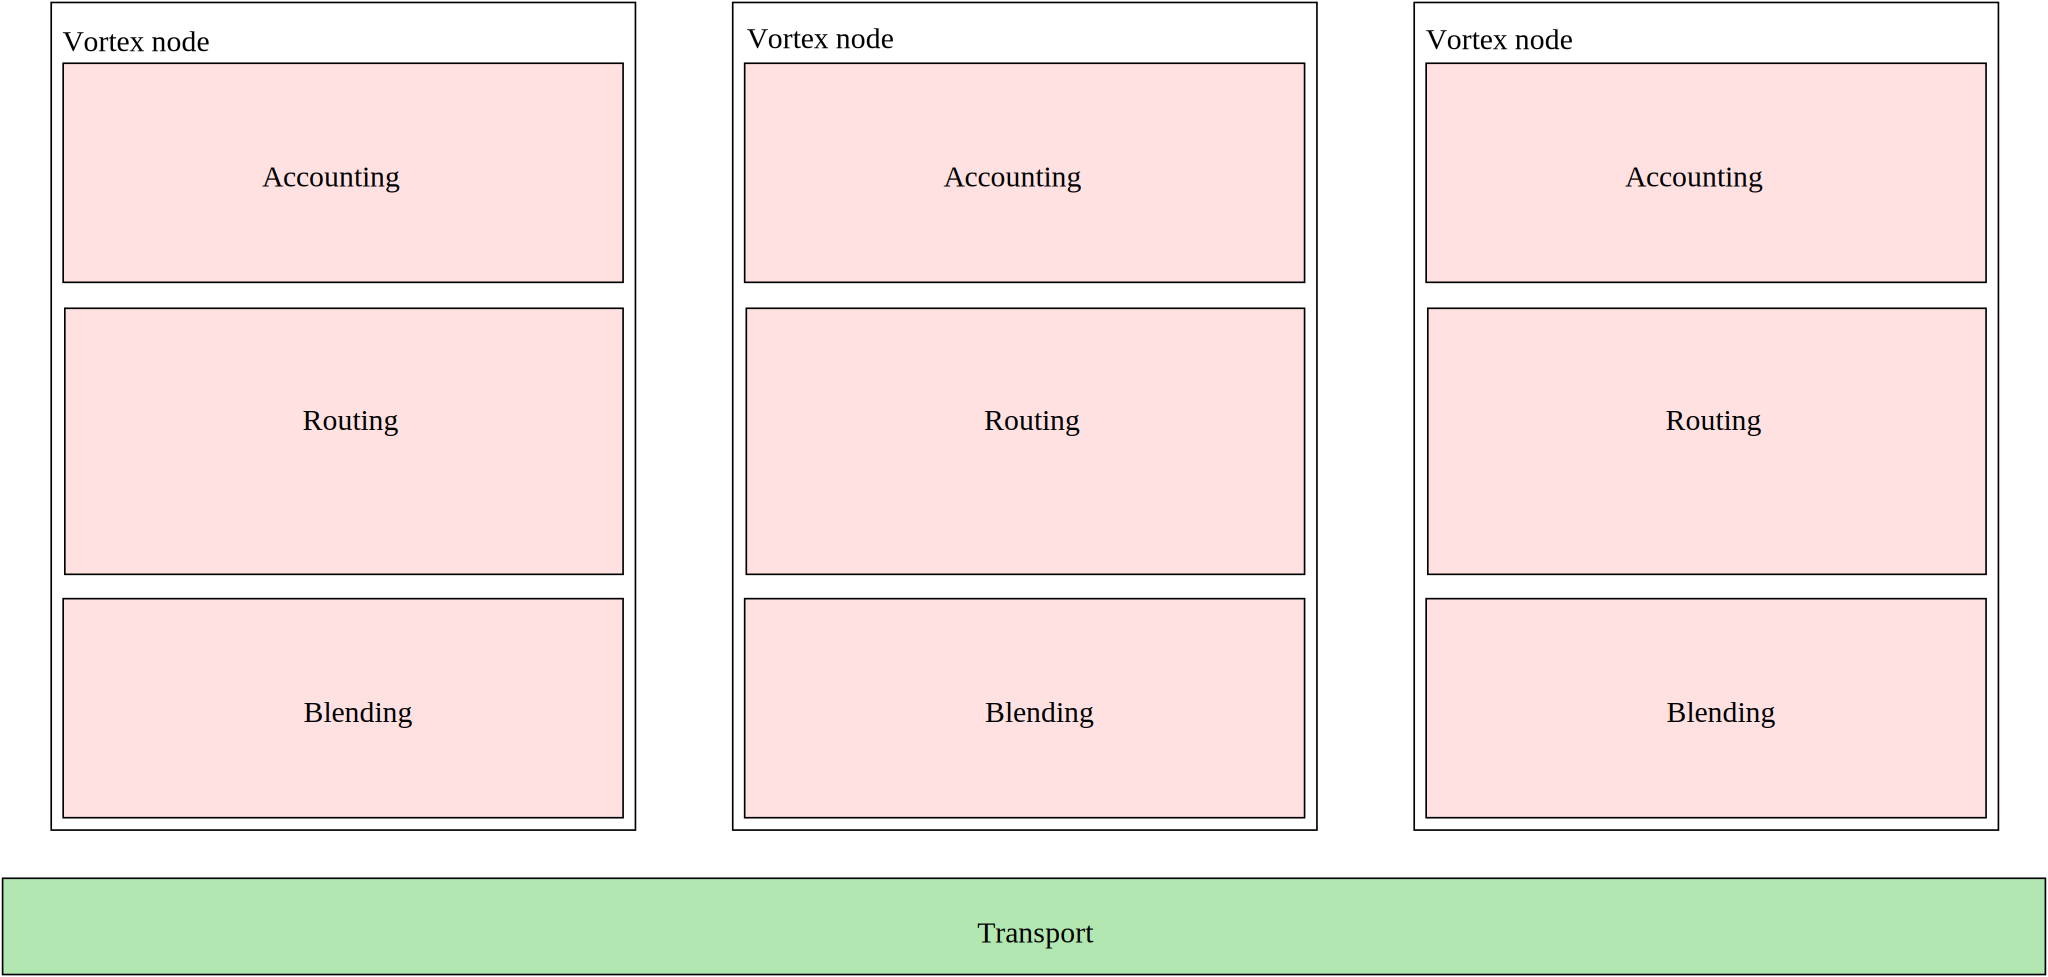
\includegraphics[width=\columnwidth]{inc/roughProtocolDesign.pdf}
	\caption{A rough protocol outline of the MessageVortex protocol}\label{fig:protocolOutline}
\end{figure}

We divide our protocol into four different layers, whereas only three are specific to the MessageVortex protocol. The lowest layer is the transport layer. As expressed earlier, dedicated protocols are easy to censor. Therefore we build our protocol on top of other suitable transport protocols. 

The other Three layers are vortex specific and do not require any infrastructure on the Internet. We elaborate further on these layers in the next section.

\subsection{Transport Layer}
For our first tests, we used a custom transport layer, allowing us to monitor all traffic quickly, and build structures in a very flexible way. This transport layer works locally with a minimum amount of work for setup and deployment. It furthermore works across multiple hosts in a broadcast domain. The API may be used to support almost any kind of transport layer.

After that, we focussed on the protocols identified in the previous sections for transport:
\begin{itemize}
	\item \defref{SMTP}
	\item \defref{XMPP}
\end{itemize}
For the prototype, we have implemented an SMTP transport agent and the respective blending layer.

\subsection{Blending Layer\label{sec:blending}}
The blending layer is taking care of multiple problems:
\begin{itemize}
	\item It is translating the message block into a suitable format for transport\\
	This translation includes jobs such as embedding a block as encoded text, as a binary attachment or hide it within a message using steganography.
	\item Extract incoming blocks\\
	Identify incoming messages containing a possible block and extract it from the message.
	\item Do housekeeping on the storage layer of the transport protocol\\
	Access protocols POP and IMAP require that messages are deleted from time to time to stay below the sizing quotas of an account.      
\end{itemize}

We define the blending layer to work as follows when receiving messages:

\begin{enumerate}
	\item Log arrival time (in UTC) on the transport layer.
	\item Extract possible blocks.
	\item Apply decryption on a suspected header block.
	\item Identify the header block as valid by querying the accounting.
	\item Extract and decrypt subsequent blocks.
	\item Pass extracted blocks and information to the routing layer.
\end{enumerate}

We define the blending layer to work as follows for sending messages:

\begin{enumerate}
	\item Assemble message as passed on by the routing layer.
	\item Using the blending method specified in the routing block, build an empty message. 
	\item Create a message decoy content.
	\item Send the message to the appropriate recipient using the transport layer protocol.
\end{enumerate}

There is no specification on the housekeeping part of the blending layer, as this part is specific to the requirements of the account owner. We do, however, recommend to handle messages precisely as if the messages would be handled on an account handled by a human. 

\subsection{Routing Layer\label{sec:routing}}
The routing layer receives the message blocks in a decrypted and authorized form from the blending layer and processes them as follows:

\begin{itemize}
	\item Build structure representing the block building and the appropriate block IDs.
	\item Schedule all Routing blocks for processing in a priority queue.
	\item Authorise all routing blocks ready for processing with the calculated block sizes.
	\item Process blocks.
	\item Send prepared building blocks to the Blending layer.
\end{itemize}

\subsubsection{Block Structure}
A VortexMessages' main block structure is a sequence of blocks. This block sequence starts with a header containing a symmetric key encrypted with the public key of the current node and a header block containing the immediate details to decrypt the subsequent blocks (if any).

A routing block follows the header block. This routing block contains the information required for subsequent routing. According to the instructions in this block, valid data blocks may be processed, assembled, and sent to a subsequent location. 

The next block is the routing log block. This block protocols the routing information of a message and is somewhat similar to an onionized variant of the received headers in SMTP.

The last part of the message is a sequence of data blocks. They contain the actual data or decoy traffic.

\subsubsection{MURBs\label{sec:murb}}
The protocol includes the capability of MURBs. Such MURBs enable a user to send a limited amount of times messages to an anonymous receiver. Such sending may be done without having any knowledge about its identity, the location, or infrastructure he is using.

A MURB in our term is an entirely prepared routing instruction built by the recipient of a message. The sender has only the routing blocks and the instructions to assemble the initial message. It does not know the message path except for the first message hops.

As a MURB is a routing block, it generates the same pattern on the network each time a sender uses it. To avoid statistical visibility, we need to limit the number of uses per MURB. As a maximum number of usages, the protocol is limited to 127 usages. This number should be sufficiently sized for automated messages. A minute pattern would disappear after 2 hours latest and an hourly pattern after five days.

For a MURB to work, the RBB has to take care that all quotas required to the route are sufficiently sized. Such sizing is hard to foresee in some cases. An RBB may query these identities from time to time to make sure that they do not deplete. Wherever possible, MURBs should be dropped in favor of multiple SURBs to avoid the dangers of MURBs.

\section{Protocol handling}
In the following sections, we outline the handling of messages we split the handling into incoming messages and outgoing messages. All handling assumes that we have a blending layer independently picking up messages as advertised in the capabilities messages.

\subsection{Block Processing}
A Block is picked up in the blending layer and then handled in the routing layer. First, we try to authenticate the message. If we can authenticate the message, we process it and add the contained instructions to a processing workspace. Unauthenticated messages may be discarded at any point.

The processing of a sending block is triggered by a routing block in the workspace, as shown in figure~\ref{fig:msgSendProcessing}. The assembly instructions are processed to collect the payload blocks. Then the encryption is applied to the message and passed on to the blending layer for processing.

\begin{figure*}[hbt]
	\includegraphics[width=0.90\textwidth]{inc/flowchart_message_sending}
	\caption{flow diagram showing processing of outgoing messages}
	\label{fig:msgSendProcessing}
\end{figure*}

\section{Sub Research Questions Roundup}
We sum up the findings of the last part regarding our three research questions and describe the next steps to be taken.

\subsection{SQ1: Technologies for sending messages maintaining unlinkability against an adversary}
We were unable to identify a single technology that withstands our adversary model entirely. The technologies were either too simple to withstand an adversary (e.g., remailers), have substantial flaws affecting their reliability (e.g., most mixes and DC networks), an active adversary could sabotage them or do not scale.

We were able to describe a rough protocol that performs far better in almost all aspects of anonymity than the solutions described in the previous sections. This comparison was always made for the adversary model given in section \ref{sec:adversary}. If we assume that the constraints of trust (only trust in sender and recipient infrastructure, whereas we always have multiple recipients) are valid, we can make the following statements regarding anonymity and unlinkability:
\begin{itemize}
	\item If an adversary identifies all involved nodes of a message and identifies all the corresponding messages and controls, all nodes except for senders and recipients nodes, he can determine message frequency, maximum message size, and message peers.
	\item If an adversary can identify all involved $i$ nodes of a sending party while controlling $j$ nodes, then he may determine a $k$-anonymity set whereas $k=i-j$ for the message set and a maximum message frequency. 
	\item If an adversary is running a node, he may identify other nodes participating in the network by analyzing peer messages.
\end{itemize}

We may safely assume that a carefully crafted message within a standard message flow is therefore unlinked from the two message peers. An adversary running a node may identify over time, possibly participating nodes, if not operating in a closed group, but he will be unable to query or use such a node without the corresponding keys. He may be able to observe such nodes, possibly view their activity, but he is unable to match messages generated.

In the next section, we will further elaborate on this protocol and analyze it. We will focus on the question of whether it is possible to create a protocol that withstands our threat model.

\subsection{SQ2: Attacking unlinkability and circumvention}
In the previous part, we identified a lot of attack schemes used to attack the anonymity of a protocol or infrastructure. While not all are technical, technicality plays a major part. We identified:
\begin{itemize}
	\item Anonymity attacks
	\begin{itemize}
		\item Hotspot attacks
		\item Side-channel attacks
		\item Sizing analysis
		\item Bugging attacks
		\item Tagging and tracing attacks
		\begin{itemize}
			\item Peer discovering attacks
			\item Traffic flow attacks
		\end{itemize}
	\end{itemize}
	\item Availability and reliability attacks
	\begin{itemize}
		\item Denial of service (DoS) attacks
		\item Censorship attacks
	\end{itemize}
	\item Non-technical Attacks
	\begin{itemize}
		\item Credibility attacks
		\item Censorship attacks
	\end{itemize}
\end{itemize}

We identified several possibilities to circumvent the attack classes listed above. Some of them, such as the bugging attack, may be countered by design (e.g., by allowing only simple messages). Others can only be countered partially in reality (e.g., DDoS attacks). We will further elaborate on the protocol and then analyze the impact of every single attack on the protocol.

\subsection{SQ3: Attack Mitigation by design}
This SQ is a part of the previous question to a certain extent. We identified that reliability and trust are key factors to a protocol. Therefore, allowing a single point of failure (SPOF) or extending trust over central infrastructures is deadly for an anonymizing protocol. Undetectability is another crucial point ignored by almost all protocols except for some aspects of Tor and some advanced forms of remailers.

When elaborating on the protocol in the next part, we will focus on introducing designs that will prohibit actions endangering anonymity. In the Result section, we will focus on all attacks, which should be mitigated by design. 


%!TeX program=pdflatex
%!TeX encoding=utf8
%!TeX spellcheck = en_US
%!TeX root = ../../messageVortex.tex


% ********************************************************************************************************
% *** Decisions and Research
% ********************************************************************************************************
\partepigraph{Thinking is the hardest work there is, which is probably the reason, so few engage in it.}{Henry Ford, American industrialist and founder of Ford Motor Co.}
\part{The  MessageVortex System}
In this part, we create a protocol called \MessageVortex{}, enabling anonymous communication. Unlike most other academic attempts, we do this on the base of an adversary, which is capable of banning our technology. We, therefore, are not able to focus solely on the anonymity property. Instead, we first collect requirements for such a system in section~\ref{sec:genRequirements}. Based on these requirements, we explain our architectural concepts and decisions in section~\ref{sec:rationale}. We then build an outline of our protocol focusing on the protocol's main properties, without going too much into implementation details. In section~\ref{sec:protocol}, we describe the protocol and its key concepts in depth. We explain all aspects relevant to the academic solution without going into implementation details.

The details of the implementation, as well as their realization in infrastructure, are in part~\ref{sec:implementation}. For operational concerns such as route building strategies, refer to part~\ref{sec:operation}.

\chapter{Requirements for an Anonymizing Protocol\label{sec:genRequirements}}
In the following sections, we first define a threat model. We then elaborate on the main characteristics of the anonymizing protocol based on the threat model. 

\begin{table*}[ht]\centering\tiny
	\label{tab:anonClass}
	%\setlength{\aboverulesep}{0pt}
	%\setlength{\belowrulesep}{0pt}
	\newcolumntype{x}[1]{!{\centering\arraybackslash\vrule width #1}}
	\rowcolors{2}{black!30}{black!10}
	\bgroup
	\def\arraystretch{1.5}%  1 is the default, change whatever you need
	\begin{tabular}{|l|l|l|p{11.8cm}|}\hline
		ID   & Category    & Short               & Description \\\hline
		RQ1  & System      & Undetectable        & Protocol nodes and their traffic should be undistinguishable from accepted nodes and traffic. \\
		RQ2  & System      & Equal Nodes         & All nodes of the system should have similar functions, capabilities, and behavior. \\
		RQ3  & System      & Zero Trust          & No trust should be imposed on any infrastructure unless it is the senders' or the recipients' infrastructure.\\ 
		RQ4  & System      & Unlinkability       & Message Requirement A message must not be linkable by an adversary to either a sender or a recipient.\\ 
		RQ5  & System      & Anonymizing         & A system must be able to anonymize sender and recipient at any point of the transport layer and any point within the system unless on the senders' or the recipients' node. \\
		RQ6  & System      & Accounting          & The system must be able to do accounting for an entity without being linked to a real identity. \\
		RQ7  & Message     & Untagable           & The message should be un-tagable (neither by a sender nor an involved intermediate node). \\
		RQ8  & Message     & Unbugable           & The message should be unbugable (neither by the sender nor by an involved intermediate node). \\
		RQ9  & Message     & Unreplayable        & A message or its behavior must not be replayable. \\
		RQ10 & Operational & Bootstrapping        & The system must allow to bootstrap from a zero-knowledge or near-zero-knowledge point and extend the network on its own. \\
		RQ11 & Operational & Algorithmic variety & The system must be able to use multiple symmetric, asymmetric, and hashing algorithms to immediately fall back to a secure algorithm for all new messages if required. \\
		RQ12 & Operational & Easy handleable     & The system must be usable without cryptographic know-how and with popular or common tools. \\
		RQ13 & Operational & Reliable            & From a user's perspective, the system must act predictably. Messages handed over to the system should reach their destination in any case. \\
		RQ14 & Operational & Transparent         & From a user's perspective, the system must act predictably. He can determine the state of a message at any given point in time. \\
		RQ15 & Operational & Available           & A user must have access to a working system and its software and updates. \\
		RQ16 & Operational & Identifiable sender & A recipient of a message should be able to authenticate a sender of a message beyond a simple authentification.\\\hline
		
	\end{tabular}
	\egroup
	\caption{Summary table of requirements}
	\label{tab:requiremnts}
\end{table*}

These requirements listed in table~\ref{tab:requiremnts} are the goal we would like to achieve. We will measure up for success or failure in section~\ref{sec:reqDiscussion}).

\section{Threat Model\label{sec:adversary}}
In this section, we define in this section two adversaries. The two adversaries are an "observing adversary (mainly doing spying) and a "censoring adversary" (Actively disrupting communication). While equal in their technical capabilities, they have different executive and legislative environments. This difference in adversaries is essential as the usage of our system differs in these two environments.

We refer to "\defref{jurisdiction}" as a geographical area where a set of legal rules created by a single actor or a group of actors apply. These actors do have executive capabilities (e.g., police, army, or secret service) to enforce this set of legal rules.

We assume for our protocol that adversaries are state-sponsored actors or players of large organizations. We assume that these actors have high funding and elaborated capabilities either themselves or within reach of their sponsor. Actors may join forces with other actors as allies. However, achieving more than 50\% on a world scale is excluded from our model. We always assume one or more actors with disjoint interests covering half of the network or more. 

We assume the following goals for an adversary:
\begin{itemize}
	\item An adversary may want to disrupt non-authorized communication.
	\item An adversary may wish to read any information passing through portions of the Internet.
	\item An adversary may wish to build and conserve information about individuals or groups of individuals of any aspect of their life. 
\end{itemize}

To achieve these goals, we assume the following properties of our adversary:
\begin{itemize}
	\item An adversary has elaborated technical know-how to attack any infrastructure. This attack may cover any attack favoring his goals, starting with exploiting weaknesses of popular software (e.g., buffer overflows or zero-day exploits) down to simple or elaborated (D)DoS attacks.
	\item An adversary may monitor traffic at any location in public networks within a jurisdiction.
	\item An adversary may modify routing information within a jurisdiction freely.
	\item An adversary may freely modify even cryptographically weak secured data where a single or a limited number of entities grant proof of authenticity or privacy.
	\item An adversary may inject or modify any data on the network of a jurisdiction.
	\item An adversary may create their nodes in a network. He may furthermore monitor their behavior and data flow without limitation.
	\item An adversary may force a limited number of other non-allied nodes to expose their data to him. For this assumption, we explicitly excluded actors with disjoint interests.
	\item An adversary may have similar access to resources as within its jurisdiction in a limited number of other jurisdictions.
\end{itemize}

As adversaries have different capabilities and goals, we should classify them among these boundaries as well. We, therefore, split up the adversaries into the following subclasses:
\begin{itemize}
	\item A censoring adversary
	\item An observing adversary
\end{itemize}

This adversary describes a powerful state-sponsored actor with very high but not unlimited powers. It serves us as a worst-case adversary.

\subsection{Observing Adversaries}
This adversary behaves like a traditional spy. He collects and classifies information while typically hiding its activities. The adversary only observes traffic and tries to extract data from the system.

Unlike the case of a censoring adversary, we imply that in most of the cases no restrictions apply for the use of anonymizing technology from a jurisdictional point of view. If restrictions apply, then such an adversary should be classified as censoring adversary, as the technology is "censored." Such classification must be done in this case, regardless of whether the adversary only tries to collect information or not.

\subsection{Censoring Adversaries}
The primary goal of this adversary is censoring messages and opinions, not within his interests. He does this, regardless of whether the activities of censorship may be observed or not. Therefore, this adversary does not necessarily cloak its activities and typically bans censorship circumventing actions as illegal.

In such environments may $k$-anonymity, as specified in \cite{k-anonymous:ccs2003}, not be sufficient for such an adversary. Instead, the \MessageVortex system must hide all activities from such an adversary.

\section{Required Properties for our Unobservable Protocol}

In this section, we collect requirements for our system. We always first list a requirement and then explain why it is essential.

\subsection{System requirements\label{sec:requirements}}

\begin{requirement}{undetectable}{Undetectable}
	Protocol nodes and their traffic should be undistinguishable from accepted nodes and traffic. 
\end{requirement}

Users are unable to limit the route of our packets through named jurisdictions. Therefore, we must protect users of \MessageVortex (users) from being subject to legal prosecution in any country. Therefore, these users need to be anonymous when sending or receiving messages. Unfortunately, most transport protocols (in fact, almost all of them such as \defref{SMTP}, SMS, \defref{XMPP}, or IP) use a globally unique identifier for senders and receivers, which are readable by any party which is capable of reading the packets (mainly the routing nodes).  

Threat model in section~\ref{sec:adversary}, we defined the adversary as someone with superior access to the network and its infrastructure. Such an adversary might attack a message flow in several ways:
\begin{itemize}
	\item Identify the sender.
	\item Identify the recipient.
	\item Identify other involved parties.
	\item Read messages passed or extract meta information.
	\item Disrupt or modify communication fully or partially. This may or may not include the possible identification of the traffic.
\end{itemize}

If users want to stay anonymous, they must protect our traffic from outside system influences. As we are unable to protect data from modification, we must hide the traffic of our application. In such a scenario, an adversary cannot block our traffic unless he is willing to disrupt communication entirely by disrupting communication of the transport protocol. 

\begin{requirement}{P2P}{equal nodes}
	All nodes of the system should have similar functions, capabilities, and behavior.
\end{requirement}

This requirement protects all involved parties from possible legal prosecution. As we are unable to introduce our infrastructure or protocols, any categorization from outside or inside would lead to an information leak. 

We have to assume that all actions taken by a potential adversary are not subject to legal prosecution. This assumption based on the fact that an adversary trying to establish censorship may be part of the government of jurisdiction. We may safely assume that there are legal exceptions in some jurisdictions for such entities. This means he may legally introduce nodes into our system.

To withstand an adversary outlined in section\ref{sec:adversary}, the messages sent even within the system requires to be unidentifiable by attributes or content. "Attributes" may include any meta information including, but not limited to, frequency, timing, message size, sender, protocol, ports, or recipient. If we want to guarantee that a node is not identifiable as an endpoint of a message, all involved nodes must carry out equivalent \defref{operation}s. As soon as we have differences between routing nodes and endpoints, we can identify participating persons at entry or exit nodes.

Furthermore, it must be impossible from an observing adversary to identify message endpoints. All nodes must look equal from the outside in terms of traffic, as well as in terms of their offered functions and behavior. 

The term "Equal nodes" does not necessarily mean that nodes must be indistinguishable. It merely means that given the functions, capabilities, and behavior of a node, no further information can be deduced.

\begin{requirement}{zeroTrust}{zero trust}
	No trust should be imposed on any infrastructure unless it is the senders' or the recipients' infrastructure.
\end{requirement}    

The requirements above protect from an adversary outside the system. Looking from the inside, an adversary may have access to much more information. An adversary will likely create nodes in an open system. As a consequence, trust in infrastructure is minimal.

In our model, we will work with suspicion into the infrastructure. As every infrastructure node learns from each transaction (e.g., the usage of the network or size of messages), we have to minimize or ideally eradicate such information gains. The main problem is that we are unable to hide peer senders or recipients when routing messages. In jurisdictions where such infrastructure usage is illegal, we need to protect the presence of our routing messages from any party not trusted. Such hiding concludes that we need to be able to control which nodes are involved when sending messages. We refer to this concept as controllable trust.

In terms of trust, we have to conclude that:
\begin{enumerate}
	\item We trust in infrastructure because it is under full control of either the sender or the recipient. If we are unable to trust these infrastructures, information may be leaked without any problems. So trusting these infrastructures is inevitable.
	\item We should not trust all other infrastructure as an adversary can misuse data passed through it.
\end{enumerate}

\begin{requirement}{unlink}{unlinkability}
	A message must not be linkable by an adversary to either a sender or a recipient.
\end{requirement}

We need a requirement guaranteeing the unlinkability between the sender and recipient from an adversary point of view. This prevents building social graphs and narrowing down groups of individuals.

\begin{requirement}{anon}{anonymization}
	A system must be able to anonymize sender and recipient at any point of the transport layer and any point within the system unless on the senders' or the recipients' node.
\end{requirement}

Unobservability requires, according to \cite{anonTerminology}, that an item of interest (\defref{IOI}) is undetectable from an uninvolved entity and anonymous for the involved entities. We therefore require: 

As a result of the architecture of today's common networks, the anonymization of a sender or a receiver is not simple. A relay may allow at least the anonymization of the original sender given trust into the proxy. By combining it with encryption, we may even achieve a simple form of a sender and receiver pseudonymity, even for a weak outside observer. This has been done in cypherpunk remailers (see section~\ref{sec:remailersAndMixnets}). If cascading more relay like infrastructures and combining it with cryptography, we may achieve sender and receiver anonymity. When introducing anonymous remailing endpoints, we may additionally achieve both simultaneously. These are the standard approaches in remailers and mixes. We have seen real-world attacks on such systems in the past, and some were successful (e.g., \cite{penetClosure}). 

\cite{anonTerminology} defines anonymity as:
\begin{quote}
	Anonymity of a subject means that the subject is not identifiable within a set of subjects, the anonymity set.
\end{quote}

If we apply our threat model, we find that we require all users to be anonymous, regardless of whether a specific user is sending messages or not. Otherwise, such a user may become subject to legal prosecution. 

\begin{requirement}{accounting}{accounting}
	The system must be able to do accounting for an entity without being linked to a real identity.
\end{requirement}

As a system may be flooded with messages, we need means to control the burden of processed messages. To separate message flows, we need means to control it by identity. Unlike other protocols, we have no identifier as we work based on the previous requirement anonymously. However: We will need some type of accounting to restrict single attackers in flooding.

\subsection{Message Requirements}
From the message point-of-view, we need to conserve privacy, which has been built up in the previous section.

\begin{requirement}{untagable}{untagable}
	The message should be un-tagable (neither by a sender nor by an involved intermediate node).
\end{requirement}

To protect a message from being followed or observed, a message needs to have certain properties. First, a message should not have, by design, any properties which can be observed when passing through the system. Any node should remove all parts which were under the control of the previous node.

\ref{req:zeroTrust} implies that a node may try to introduce such features into the message. As we cannot keep a node from doing so, we can define that such tags must be removed by the next node. 

\begin{requirement}{unbugable}{unbugable}
	The message should be unbugable (neither by the sender nor by an involved intermediate node).
\end{requirement}

Another way of breaking anonymity is that, instead of following a message through the system, an adversary may modify (bug) it so that the receiving or any intermediate node leaks its presence. In traditional messaging such bugging is done by introducing remotely hosted data or by introducing revocable certificate operations into the message stream and then observe the VA of a PKI for respective OCSP calls or CRL accesses. Our protocol handling must not depend on such external lookup mechanisms to ensure that bugging is not possible:

As with \ref{req:untagable}, a recipient or an intermediate node may be identified by a download or lookup behavior of a recipient or any intermediate routing node.  

\begin{requirement}{unreplayable}{unreplayable}
	A message or its behavior must not be replayable.
\end{requirement}

In a generic sense a node may also replay a message to highlight a messages property (e.g., the path or a size), which leads us to the following requirement:

\subsection{Operational Requirements}
In order to be realistically operated, our system needs to fulfill some additional requirements.

\begin{requirement}{boot}{bootstrapping}
	The system must allow to bootstrap from a zero-knowledge or near-zero-knowledge point and extend the network on its own. 
\end{requirement}
Up until here, we described a system that is not centrally controlled. If not relying on broadcast domains, which is not feasible on a global scale, each node needs to know other nodes that may be contacted for routing purposes. We refer to the initial process of collecting routing nodes as bootstrapping.

\begin{requirement}{algVar}{algorithmic variety}
	The system must be able to use multiple symmetric, asymmetric, and hashing algorithms to immediately fall back to a secure algorithm for all new messages if required. 
\end{requirement}

It is quite common that weaknesses in algorithms are discovered. We may, therefore, not rely on a single algorithm. Instead, we must create a protocol supporting crypto agility, as described in \cite{bsiPostQuantum}.

\begin{requirement}{easy}{easy handleable}
	The system must be usable without cryptographic know-how and with popular or common tools.
\end{requirement}

Academic systems are usually not known for focusing on user-friendliness. Users, on the other hand, are not known for their willingness to give up a lot of functionality or usability in trade for security. If we want that our system is used, many users need to use the system. This would lower the bar for bootstrapping and increase the size of anonymity sets. We, therefore, conclude that the system must be easy to handle for a user. Usually, this would be a decision related to a GUI or an end-user application but not to a system. However, if we want our system to be easy to handle, we need to take this as a requirement into account.

\begin{requirement}{reliable}{reliable}
	From a user's perspective, the system must act in a predictable manner. Messages handed over to the system should reach their destination in any case.
\end{requirement}

Any message-sending protocol needs to be reliable in its functionality. If the means of message transport are unreliable, users tend to use different means for communication\cite{zhou2011examining}. 

\begin{requirement}{transparent}{transparent}
	From a user's perspective, the system must act in a predictable manner. He is able to determine the state of a message at any given point in time.
\end{requirement}

Transparent behavior is a prerequisite for reliability. If something is generating a  behavior, but a user is unable to determine the reason for it (i.e., if a user is expecting a different behavior), he usually assumes a malfunction. Therefore, "reliable" means not only stable by its behavior. It also means diagnosable. A user's perception will not be "reliable" if he is not able to determine causes for differences in observed and expected behavior (e.g., \cite{nicholson2003assessing}).

\begin{requirement}{available}{available}
	A user must have access to a working system and its software and updates.
\end{requirement}

If a user should be able to use the system, he needs access to other nodes and the required software, as well as its updates. This has to be considered even in an environment with a censoring adversary. So the system needs to be available.

Availability, in this specific context, may have two meanings, which do differ. A system is available if\ldots
\begin{enumerate}
	\item a sender and a recipient have (or may have) the means of using it.
	\item the infrastructure provides the service (as opposed to: "is running in a degraded or faulty state and, therefore, unable to provide the service").
\end{enumerate}

\begin{requirement}{senderId}{identifiable sender}
	A recipient of a message should be able to authenticate a sender of a message beyond a simple authentification.
\end{requirement}

A messaging system offering unlinkability may offer sender anonymity from a recipient's perspective. If so, a sender should be identifiable in such a way, that a classification of senders is possible for a legit recipient, and impersonation is not achievable. It is important to understand that an identifiable sender does not necessarily mean that users can identify a sender as a specific party. It only means that two senders may be identified as the same sender.

\chapter{Rationale\label{sec:rationale}}
In this chapter, we set the course for our system. We explain why we built the protocol the way it is. We try to elaborate on our decisions and explain why the system is not built differently.

The system we describe is a four-layered system (transport, blending, routing, and accounting layer) in which each layer fulfills a specific duty. The transport layer is equal to an unmodified, common internet data transport protocol. The blending layer inserts and extracts our protocol messages into the transport layer. The routing layer does disassemble and reassemble the messages received and applies specially crafted operations, and the accounting layer keeps track of quotas and protects the resources of the system. The three \MessageVortex{} layers (all layers except "transport") run on common internet end-user devices such as mobile phones or tablets.

\section{System Design and Infrastructure}
All anonymity systems listed in part~\ref{sec:systems} have in common that they do rely on dedicated servers providing an anonymity related service. Such specialized servers make operators of such servers vulnerable in an environment where a censoring adversary (as described in section~\ref{sec:adversary}) exists. Our approach should, therefore, be different. Instead of creating our own protocol, we describe a system where we use preexisting standard servers without modification. If we succeed to piggyback such a protocol invisibly, we may inherit the regular usage of this infrastructure as decoy traffic. Piggybacking and mimicking of protocols is not new. Protocols such as Skypemorph\cite{mohajeri2012skypemorph} or pluggable transports for Tor (e.g., Meek, FTE, or OBFS4) use this technology successfully for censorship circumvention.

We will do this piggybacking in a protocol-agnostic manner. On the protocol level, this requires that we separate embedding of messages into the transport protocol from the rest of the system. To do this in such a way makes the system even harder to observe as routing graphs taking multiple protocols into account increase the complexity exponentially through their different properties.

The content of the message in the transport layer protocol is provided by the routing node and not by anyone else. This restriction is based on the fact that if we allow anyone else except the routing node itself to control visible aspects of the transport layer message, the system could be misused for sending transport layer messages. To give an example: Such a system could be misused for blackmailing of a user not participating in the system. We simply create a message obfuscating the source and then exit the system by embedding the true blackmailing message. 

As we rely on third-party infrastructure with our approach, now we have to take special care when designing our approach not to violate requirement \ref{req:zeroTrust}. For obvious reasons, a direct connection between the sender and recipient via any named transport protocol would violate the requirement \ref{req:unlink}. A single intermediate node would minimally imply trust in this node and its anonymization capabilities, which is not acceptable due to the requirement \ref{req:zeroTrust}. When using multiple nodes, other anonymization protocols typically use three to five intermediate nodes due to their arguing. Typically we have at least three anonymization nodes for obvious reasons and sometimes an entry and exit node summing up to five nodes. This implies that the routing of our protocol is required. As we have an \ref{req:zeroTrust} policy, decisions for routing may no longer take place on the routing node but must be dictated externally. 

For routing, we will use end-user devices. This decision is further backed by the requirement \ref{req:P2P}. It, however, opposes the requirement of \ref{req:reliable}, as such system participants are likely to be unreliable due to missing network connectivity, device failure due to drained batteries, or simply because they no longer participate in a network. To counter this, we implement measures on the message level.

\section{Message and Routing}
One of the biggest weaknesses of all protocols is the information leakage they have by design and the inability to restrict access to their functionality. We will build the messages with the following design guidelines:
\begin{itemize}
	\item No routing controlled content shall survive a hop.\\
	For us, this means that by design, a message is received and dismantled. Any content visible or manipulable by the previous node must be removed. Only new content or content inaccessible to the previous node may be used to build new messages. Following this criterion, we automatically fulfill the requirement \ref{req:untagable}.
	\item A routing node may efficiently identify a message sender.\\      
	The sender must be efficiently identifiable. At first sight, this requirement is non-fitting as it opposes heavily to \ref{req:anon} and \ref{req:unlink}. On the other hand, not providing these means makes it next to impossible to create a system that may not be misused and flooded. As the identification is pseudonymous, it must be short-lived, and multiple identities of the same sender must not be linked to each other. We will refer to this identity as an ephemeral ID (\defref{eID}). This \defref{eID} is handled in such a way that not complete decoding of the message is required to authorize the user. Instead, we build a message in such a way that tamper-proof, small-sized parts of the message are decoded first, and possibly bloated message content may be decoded after it is clear that the content is acceptable. If we assign "costs" to the creation of \defref{eID}s, it effectively protects the system from flooding.
	\item The routing \defref{operation}s must not leak more information than the next hop.\\
	We will apply a transformation on each routing hop to the message. This prevents following the message throughout the system. In most of the systems, messages are mainly disassembled and reassembled or onionized. The traffic is then cloaked in mimic traffic, making it impossible for an outside observer to identify message flows. The node generating the traffic is, however, well aware of the true message flow. In our system, we will add, instead of mimicking traffic, redundancy information (or remove it). By doing so, a routing node has no longer the insight which part of the traffic is relevant to the message and which not. We may, furthermore, introduce the possibility of distributing the message content throughout multiple paths in such a way that each path has not sufficient content to rebuild the message. In fact, depending on the complementing missing message, any content may be valid. 
	\item Messages are protected from being replayed.\\
	In former systems, message paths were highlighted by injecting additional information. Our system is already protected from such injections by the \defref{eID} concept, which identifies the sender. There are, however, other means to highlight traffic. An adversary may either inject message payload (corrupting the message flow) or replay the message. While we cannot keep anyone from sticking to rules, we may at least implement replay protection. Furthermore, we may later observe that we are able to control willingly induced, size mismatching content.
	\item Messages in the routing system are "store and forward" .\\
	All synchronous routing systems have in common that message observation is relatively easy for an outside or inside observer unless mimick routes are used. This is why we allow the message to be stored and picked up or sent at a later stage. 
	\item Use the Reed-Solomon-Function as the main routing \defref{operation}.\\
	Originally \cite{reed1960polynomial} introduced a system allowing the use of polynomes to create error-correcting codes. In \cite{chaum1988multiparty} \citeauthor{chaum1988multiparty}, they have shown that the codes are suitable for distributing data assuming enough parties are honest and not malfunctioning. Unlike \citeauthor{chaum1988multiparty} proposition, we are not using the Reed Solomon function to achieve anonymity or privacy. Instead, we use it for decoy traffic generation. We are splitting a message into multiple parts at several points when routing and assemble it again on different nodes. By doing so, we achieve two vital things. First, we introduce the possibility of recovering errors due to misbehaving nodes, and secondly, the real traffic can no longer be differentiated from decoy traffic. The \defref{operation} has proven to be insecure as it leaks properties of the operation applied in the result. We will show this in section \ref{sec:analysisReedSolomon}. Thus, We hardened the operation to remove the negative effects.
	\item \MessageVortex{} must provide a variety of algorithms and \defref{operation}s to build a message.\\        
	As all systems and algorithms applied to the system may be weakened or fail, a system needs to have the possibility to choose from multiple algorithms, protocols, and infrastructures. This choice should be made by a trustworthy system that restricts us to either the sender or the receiving system. The German Federal Office for Information Security (BSI) makes in \cite{bsiPostQuantum} recommendations for systems and protocols, which we will follow.
	
	The main text can be boiled down to the following recommendations:
	\begin{itemize}
		\item A protocol or system should be crypto agile.
		\item A protocol or system should use hash-based signatures for updates.
		\item The document furthermore recommends using symmetrical keys with a key length of 128 bit or more.
		\item The document recommends a combination of big long term keys and small short term keys.
		\item The document recommends using a combination of multiple independent algorithms in cascaded forms so that if one algorithm fails, the other one is still able to protect the data.
		\item For key exchange, BSI recommends lattice-based cryptography.
	\end{itemize} 
\end{itemize}

\section{Summarizing Chosen Approaches for \MessageVortex\label{sec:reqSummary}}
In this section, we have taken the following decisions for \MessageVortex:
\begin{itemize}
	\item Piggybacks common protocols.
	\item Does not require specialized hardware within the Internet.
	\item No proprietary systems on the Internet.
	\item Runs on commodity hardware.
	\item Sends messages in an asynchronous mode.
	\item Creates unidentifiable decoy traffic by using a Reed-Solomon-Function.
	\item Have no strict message size and avoid strictly increasing or decreasing sizes in any type of message or message part.
	\item Does not enforce specific attributes such as transport protocol, message size, message timing, or providers.
	\item Run special routing \defref{operation}s instead of traditional mixing and recombination methods.
	\item Offer a choice of algorithms to use when routing.
\end{itemize}

\begin{figure}[ht]
	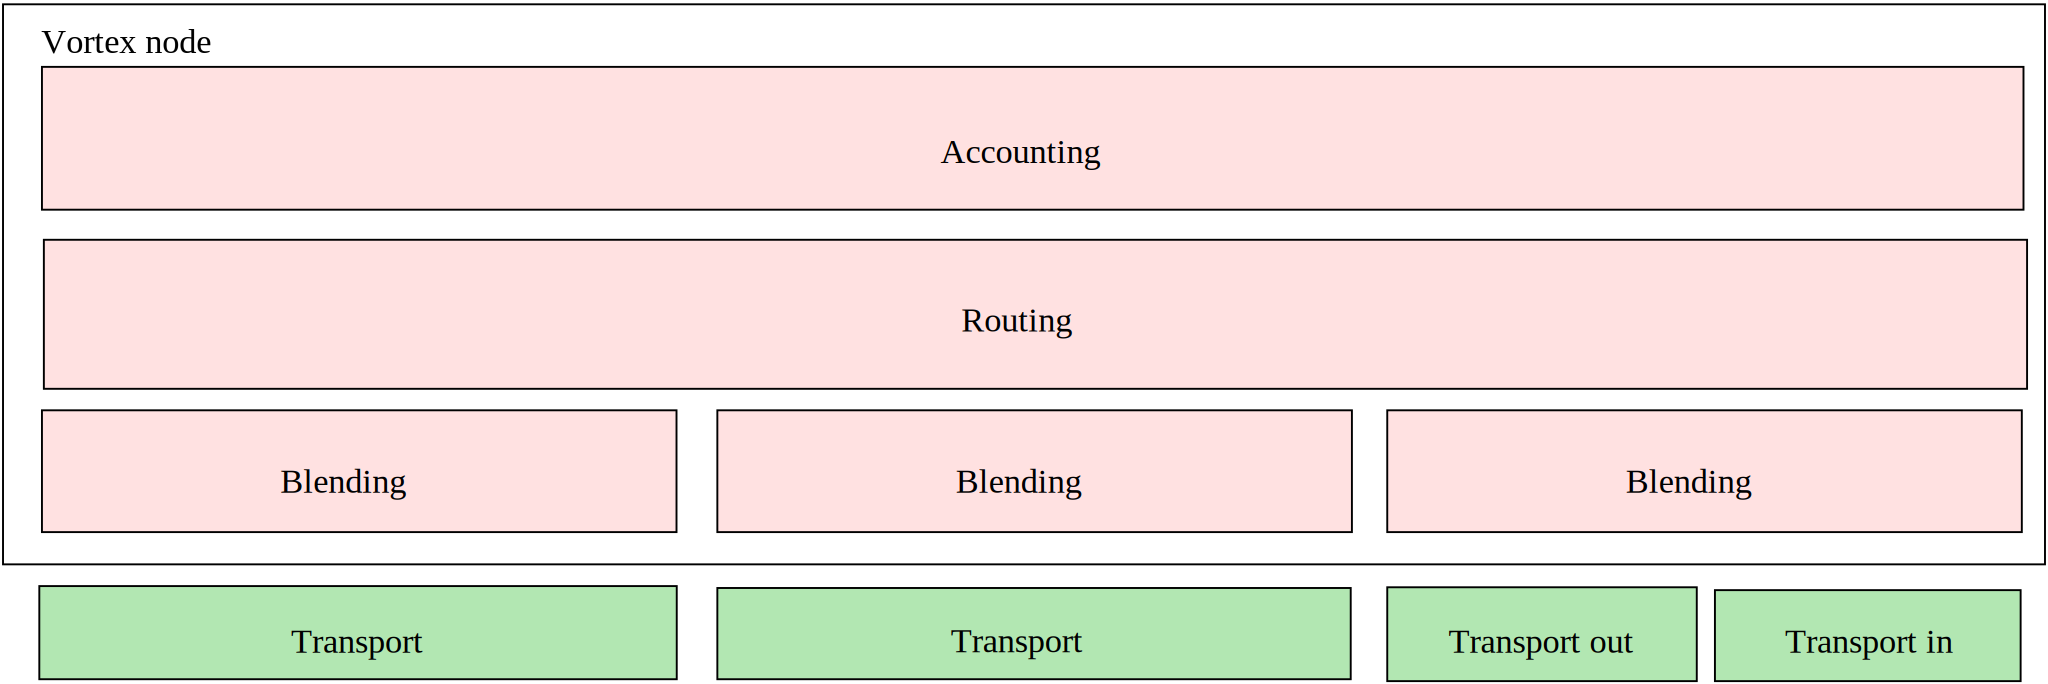
\includegraphics[width=\textwidth]{inc/layerDesign}
	\caption{The protocol layers}
	\label{fig:protocolLayers}
\end{figure}

The protocol is a four-layer protocol, as shown in figure~\ref{fig:protocolLayers}. We communicate with standard protocols, which we refer to as the transport layer. While included in the message flow, they do not form a part of the \VortexNode. The \VortexNode{} itself consists out of the three layers ``Blending'', ``Routing'', and ``Accounting''.

The blending layer is the bridging part linking a transport layer to the \VortexNode{}. It injects and extracts messages from the transport layer and passes the extracted messages to the routing layer. It may be either used as a protocol bridge (e.g., in the case of XMPP) or act as a sophisticated router (e.g., in the case of the email protocols, where mails are fetched or received on push event via POP3 or IMAP while sending messages using SMTP).

The routing layer receives unified standard messages from the blending layer processes them, possibly extracts messages for local delivery, and passes subsequently created messages to the blending layer.

This design is definitely implementable on a consumer device. On the other hand, it is scalable and suitable for a clustered environment. Blending can be done in a stateless manner, is even suitable for serverless computing, and thus largely scalable. Routing may be implemented either with horizontal partitioning along with a set of \defref{eID}s or on a serverless base with a unified storage in the background. The accounting layer acts as a controller and may be implemented as well as stateless service with a minimal NOSQL-storage for all \defref{eID}s. 

\chapter{Protocol}\label{sec:protocol}
\MessageVortex{} is a protocol piggybacking standard transport protocols somehow similar to S/MIME\cite{rfc2015} or PGP\cite{PGP}. Unlike these protocols, we need the capability to keep the presence of our messages secret.  The message itself should only be visible to an intended node.\MessageVortex{} itself is agnostic to the transport, but we do require appropriate blending to hide within the transport protocol. The information processed on a node and its associated meta-information should not leak any information about the processed message. 

Our system sends so-called \VortexMessages. These messages are hidden within a transport protocol (e.g., SMTP or XMPP) with a blending mechanism (e.g., the steganographic algorithm F5) and extracted by a blending layer. The extracted \VortexMessage{} is handed over to a routing layer. The \VortexMessage{} itself contains a header block, a routing block, and possibly some payload blocks. The header block contains all the information required to protect the system. The routing block contains instructions (so-called ``\defref{operation}s'') how the payload blocks have to be processed and where to send the resulting blocks. Those \defref{operation}s are one of the keys as information leaking happens in this step in most of the systems. We, therefore, crafted all \defref{operation}s very carefully to keep as much information secret as we could. These \defref{operation}s are the key to the system as they allow us to increase and decrease the size of a message without leaking what part of the data is a decoy and what not.

A payload may either be kept by the system for later processing with other messages, processed (possibly with different) payload blocks, or displayed to the "local user" as a message.

The general idea of the protocol is to form a network from nodes that mix and route messages between the sender and receiver. A routing block builder (\defref{RBB}), which is typically identical to the sender, has full control over almost all attributes of the message, and nodes are unable to learn anything from the message while routing. Each user has a node, and there may be additional nodes (public routing nodes) without a user connected to it. 

The message is either onion-like encrypted, split into parts and remerged, or blown up with redundancy information. 

This behavior results in a mixing like a system with a decoy generation in which even decoy generating nodes are unable to differentiate between real traffic and decoy as all blocks always contain parts of the message. Routing decisions are controlled by the builder of the routing block, and redundancy is possible and controlled by the routing block builder to make the system more stable.

In the following sections, we describe this protocol in detail. First, we build a terminology implicitly used in the previous chapters. Then we describe the key concepts and techniques of the protocol without in-depth analysis or reasoning. Implementation and operational aspects are discussed in part~\ref{sec:implementation} and part~\ref{sec:operation}. 


\section{Protocol Terminology}
For our protocol, we use the following terms:
\begin{itemize}
	\item \textbf{\defref{Sender}:} The user or process originally composing the message.
	\item \textbf{\defref{Recipient}:} The user or process destined to receive the message in the end.
	\item \textbf{\defref{User}:} Any entity, running a \MessageVortex{} node.
	\item \textbf{\defref{Router}:} Any node which is processing the message. Please note that all \VortexNode{}s are routers. This includes the senders' and recipients' node.
	\item \textbf{\defref{Message}:} The "real content" to be transferred from the sender to the recipient.    
	\item \textbf{\defref{VortexMessage}:} The encoded message passed from one node to another one. The \VortexMessage{} is considered before any embedding takes place. If embedded, we refer to such a message as "embedded \VortexMessage".
	\item \textbf{\defref{Payload}:} Any data transported in a \VortexMessage{} between routers with exception to the routing and header block, regardless of the meaningfulness or relevance to the \VortexMessage.
	\item \textbf{\defref{Decoy traffic}:} Any payload transported between routers that have no relevance to the message at the final destination.
	\item \textbf{\defref{Identity}:} A tuple of a routable address and a public key. This tuple is a long-living tuple but may be exchanged from time to time. An Identity is always assigned to a node, but one node may have multiple identities. 
	\item \textbf{\defref{eID}:} An identity created on any node with a limited lifetime anyone possessing the private key (proven by encrypting with it) is accepted as representative of that identity.
	\item \textbf{Routing Block Builder (\defref{RBB}):} An entity, which is building a routing block. Typically identical to either sender or recipient.
\end{itemize}

\section{Key Components}
The following sections list some of the key components of the system. Their understanding is essential for the understanding of the protocol as a whole. 

We first describe a single node and its identity. This node is always equivalent to a potential recipient. 

We then introduce the concept of \defref{workspace}s and ephemeral identities. These concepts are essential for the routing and accounting layers. They dictate memory and storage requirements and lay a foundation for the routing layer.

A node always consists of three layers and one or more transports connected to it. The understanding of their inner workings is essential to the understanding of the project as a whole. We emphasize on their main function and their inner workings without going into implementation details. These details are further discussed in part~\ref{sec:implementation}. We mainly focus on the data and the high-level processing done within these layers.

\subsection{Nodes and their identities}
We refer to a \VortexNode{} (node) as a system run by an individual containing a processing software processing \VortexMessages. Each node is connected to a transport layer protocol service (e.g., an IMAPv4 server as an endpoint for email or an XMPP server). 

Each node $o$ has at least one identity reflected by an asymmetric key pair $K_{host_o}$. Any node $p$ communicating with node $o$ must have the public key  $K^1_{host_o}$ of the node.

A node requires the key $K^1_{host_o}$ to encrypt a message for node $o$. This key know-how enables environments with censoring adversaries to withstand probing attacks, as, without the knowledge of such keys, no reply from a node is received. The transport endpoint itself is not secret. The usage as \VortexNode, however, is kept secret as long as the key is not known.

The protocol itself has the possibility to answer clear-text requests. So-called ``public nodes'' (see \ref{sec:vortexNodeTypes}) make use of such messages. They are, however, an exception. In general, all \VortexMessages{} are encrypted.

\subsection{Workspaces and Ephemeral Identities}
We dumped the approach for a system global unified storage for all message processing as such a design would allow an adversary to flood our storage. Instead, we introduced temporary storages suitable for a set of transaction belonging to a single identity or limited set of entities which collaborate. In our system, every transaction on a nose is assigned to an ephemeral identity (\defref{eID}). An \defref{eID} has a limited lifetime and is represented by an asymmetric key pair and has to be created on each \VortexNode{} taking part in a message processing. Each \defref{eID} has a storage assigned to which we refer as ``\defref{workspace}''.

An \defref{eID} is unique on every host and created on each \VortexNode{} by the routing block builder (\defref{RBB}). To create an \defref{eID}, an \defref{RBB} first sends a message with only a header block to the respective \VortexNode. The request contains the new identity, a reply block, and a request to create a new identity. The receiving \VortexNode will then typically sends a challenge back. A challenge may be the start of a hash bit sequence (also referred to as "puzzle"). The requester has then to resend the request with a header block. The requester must insert additional data in such a way that the start hash in its binary form matches the bit sequence provided. Another possibility is to request a payment in cryptocurrency. This allows us to commercialize routers in some countries where the usage of such routers is generally allowed.

The length of the requested bit sequence is chosen by the accounting layer at its own will. If the request is not answered in a given time, the \defref{eID} will be discarded. Analogous to an SYN-Flood attack, an adversary may try to overwhelm a \VortexNode{} with \defref{eID} creation requests. Such flooding will be much more costly for the adversary than for the \VortexNode{}, and such a node may decide to temporarily no longer accept new \defref{eID} requests without affecting already existing \defref{eID}s.

Each \defref{eID} has a lifetime, a maximum number of messages to be processed, and a maximum number of bytes to be sent assigned to it. The lifetime of an \defref{eID} is typically days and maybe up to a low number of months. Lifetimes may not be extended and are defined by the sender of the request. A node may accept or decline the request if the lifetime of the request or the state of the node does not meet its expectation. The puzzle sent in return may be a fixed value or related to the nodes' current state and load.

This system guarantees that a sender must invest considerable work (in terms of CPU time required) prior to using resources of a \VortexNode. A \VortexNode{} may raise the complexity of its puzzles when having a  high load. This allows for a single user to still obtain an \defref{eID} while increasing costs for an attacker considerably. Even if someone floods a node with new \defref{eID}s, already created \defref{eID}s are not affected as their \defref{workspace} has already been allocated.

The \defref{workspace} itself contains chunks of the messages (payload blocks) mapped to \defref{ID}s and \defref{operation}s. The \defref{operation}s transform one or more source \defref{ID}s onto one or more target \defref{ID}s. Any of these payload blocks may be assigned to a subsequent message as payload block by a routing block. An \defref{operation} or a payload block share the lifetime of the respective message header. If \defref{operation}s overlap in output blocks the newest \defref{operation} (arrived latest) wins. Arriving \VortexMessages{} map their payloads onto \defref{ID}s of the respective \defref{workspace} of the \defref{eID}. to allow such mapping the first IDs are special \defref{ID}s either mapping to the \defref{ID} 0 (message for local delivery) or \defref{ID}s 1-127 (always reflect the current message [ingoing or outgoing]).

This concept has certain downsides related to the expiry of \defref{eID}s. We will address them in section\ref{sec:newEID} and section~\ref{sec:replaceMURB}.

\subsection{Protocol Layers}
As already introduced in \ref{sec:reqSummary}, the protocol is built on multiple software layers. On the logic side, the protocol is split into two parts:
\begin{enumerate}
	\item Transport Layer\\
	Standard Internet infrastructures provide this layer. The primary goal is to hide or blend our protocol into regular traffic within that layer. Typical examples for such layers are SMTP or XMPP servers.
	\item Blending and subsequent layers (the Vortex infrastructure)\\
	Any user of the Internet may provide these layers. Since these layers may be only Vortex routing nodes or valid endpoints, the nodes may or may not be publicly known. In a first implementation, we build this system as a standard Java application. The primary goal is to compile it to native code afterward and run it on an SoC like infrastructure such as a RaspberryPi or port it to an android device.
	
	We may further split the Vortex infrastructure layers into
	\begin{enumerate}
		\item dBlending layer\\
		This layer receives messages from the Vortex system and creates transport layer conformant messages and vice-versa. In an ideal case, the messages generated by this layer are indistinguishable from any regular message traffic of the transport layer, and the embedded message is only detectable by the receiving node.
		\item Routing layer\\
		The routing layer disassembles and reassembles messages. 
		\item Accounting layer\\
		The accounting layer has three jobs. First, he has to authorize the message processing after the decryption of the header block by the blending layer. Secondly, he handles all header request blocks and the reply blocks. And third, it keeps track of the accounting regarding the sent messages. Its main purpose is to protect the system from misuse or flooding.    
	\end{enumerate}
\end{enumerate}

In total, we have four layers. The bottom-most layer consists of unmodified standard infrastructure for transport within the Internet, and the three layers on top build a single \VortexNode.

\subsection{Transport Layer}
The transport layer is a standard protocol within the Internet. It is neither a \MessageVortex{}-specific infrastructure, nor has it been modified for the purpose. Instead, it serves the purpose as a store and forward medium. This medium solves two major problems. First, no NAT traversal technology such as "TCP hairpins" or "hole punching" is required. And secondly, it compensates for short outages due to regional routing problems to the end-user.

A transport layer should have some generic properties:
\begin{itemize}
	\item Widely adopted 
	\item Reliable
	\item Symmetrical built 
\end{itemize}

For a more detailed description of the criteria, see section~\ref{sec:transportCriteria}.

For our first tests, we used a custom transport layer, allowing us to monitor all traffic quickly, and build structures in a very flexible way. This transport layer works locally or in a broadcast-based network with a minimum amount of work for setup and deployment. The API we used may, however, be used to support almost any kind of transport protocol.

In section~\ref{sec:transportProtocols}, we make a short analysis going through some common protocols outlining the strength and weaknesses of common transport protocols within the Internet.

After that, we focussed on the protocols identified in the previous sections for transport:
\begin{itemize}
	\item \defref{SMTP}
	\item \defref{XMPP}
\end{itemize}
For the prototype, we have implemented an SMTP transport agent and the respective blending layer.

\subsubsection{Blending Layer\label{sec:blendingLayer}}
The blending layer is taking care of multiple problems:
\begin{itemize}
	\item It is translating the message block into a suitable format for transport\\
	This translation includes jobs such as embedding a block as encoded text, as a binary attachment or hide it within a message using steganography. Another demanding task in this context is to create credible content for the transport message itself.
	\item Extract incoming blocks\\
	Identify incoming messages containing a possible block and extract it from the message.
	\item Do housekeeping on the storage layer of the transport protocol\\
	Access protocols such as POP and IMAP require that messages are deleted from time to time to stay below the sizing quotas of an account. To manage this transport layer account is the job of the blending layer.
\end{itemize}

There is no specification on the housekeeping part of the blending layer, as this part is specific to the requirements of the account owner. We do, however, recommend to handle messages precisely as if the messages would be handled on an account handled by a human. This means that some messages. 

The blending is currently done by merging the \VortexMessage using either F5 as described in \cite{f5} or by doing plain blending, which is a binary embedding. This means that we require jpeg images included in the SMTP message. 

\paragraph{Processing of a Message received from the Transport Layer}~\\
We define the blending layer to work as follows when receiving messages:
\begin{enumerate}
	\item Log arrival time on the transport layer.
	\item Extract possible \VortexMessage.
	\item Apply decryption on a suspected header block of \VortexMessage.
	\item Identify the header block as valid by querying the accounting layer.
	\item Extract and decrypt subsequent blocks.
	\item Pass extracted blocks and information to the routing layer.
\end{enumerate}

\paragraph{Processing of a Message received from the Routing Layer}~\\
We define the blending layer to work as follows for sending messages:
\begin{enumerate}
	\item Assemble message as passed on by the routing layer.
	\item Using the blending method specified in the routing block, build an empty message. 
	\item Create a message decoy content.
	\item Send the message to the appropriate recipient using the transport layer protocol.
\end{enumerate}

\paragraph{Credible Content Creation for the Transport Layer}~\\
One of the most demanding tasks of the blending layer is to create transport protocol messages. In \cite{oakland2013-parrot}, \citeauthor{oakland2013-parrot} expresses that it is easy for a human to determine decoy traffic as the content is easily identifiable as generated content. While this is up to all that we know true, there is a possibility here to generate "human-like" data traffic to a certain extent. For the blending layer, it is not necessarily required to mimic human messages. Instead, the blending layer may generate messages such as password recovery messages, monitoring messages, and even \defref{UBE}-like content. All these messages have required properties in common. First, all of them are machine-generated messages which are modified quite often. All of these messages are known to be sent and possibly adapted individually. 

For the blending itself, we required a steganographic algorithm. After reviewing the options, we decided to go for F5\cite{f5} as a steganographic algorithm. It is a reasonably well-researched algorithm, which attracted many researchers. The original F5 implementation had a detectable issue with artifacts\cite{F5broken} caused by the recompression of the image. This issue was caused only due to a problem in the reference implementation, and the researchers have provided a corrected reference implementation without the weakness.

We looked for other steganographic algorithms, but were unable to find any other suitable algorithm apart from F5, which fulfilled the following set of criteria:
\begin{itemize}
	\item Unbroken.
	\item Researched.
	\item Suitable for embedding in lossy compressed, common image formats (e.g., jpeg).
	\item An implementation or a well-specified algorithm exists.
\end{itemize}

We decided to keep our plain embedding algorithm in the implementation. It already requires an in-depth analysis or a human to detect embedding, and the message itself is, even if detected, well-protected. Its biggest most strength is, however, its efficiency. This algorithm is, however, only suitable for public nodes matching up to an observing adversary (as defined in section~\ref{sec:adversary}). It must not be used in environments where a censoring adversary is suspected.

When using F5, jpeg images are required. Imagery requires to be at least eight times the size of the message embedded. Unlike other approaches harvesting random pics or obtaining them from a local repository, we recommend using machine-generated images such as rendered content. We recognize that custom Gravatars, router and usage graphs of services, or render services are suitable imagery material for our purpose. The message content would obviously be machine-generated content and not being suspect. This would effectively render the dead parrot problem as described in \cite{oakland2013-parrot} ineffective. 

\subsubsection{Routing Layer\label{sec:routingLayer}}
A routing layer needs to receive all payload and routing blocks, and process them (For an exact outline of the routing block, see section~\ref{sec:vortexMessage}). These blocks are stored in a suitable list within the \defref{workspace} of the \defref{eID} identified by the header block.

Within the routing block, we find a set of instructions, next \VortexNodes information, and the encrypted routing blocks for the messages to be assembled. A simplified representation of a routing block is shown in figure~\ref{fig:mathRoutingSimplified}.

\begin{figure}[!ht]
	\begin{align}
	\mathbf{ROUTING_o}           = & \langle [ \mathbf{ROUTINGCOMBO} ] *, \mathbf{replyBlock},mapping* \rangle\\  
	\mathbf{ROUTINGCOMBO}        = & \langle processIntervall, K_{peerN+1}, recipient, \mathbf{nextMP}, \mathbf{nextHP}, \nonumber \\
	& \mathbf{nextHEADER}, \mathbf{nextROUTING}, \mathbf{assemblyInstructions} \rangle\\
	\mathbf{PL}                  = & \langle \text{payload octets} \rangle *\\ 
	\mathbf{nextMP}              = & E^{K^1_{host_{o+1}}} \left( K_{peer_{o+1}} \right)\\
	\mathbf{nextHP}              = & E^{K^1_{host_{o+1}}} \left( K_{sender_{o+1}} \right)\\
	\mathbf{nextHEADER}          = & E^{K_{sender_o}} \left( \mathbf{HEADER_{o+1}} \right)\\
	\mathbf{nextROUTING}         = & E^{K_{sender_o}} \left( \mathbf{ROUTING_{o+1}} \right)\\    
	\mathbf{operations}          = & \langle \text{list of operations} \rangle \\
	\mathbf{assembyInstructions} = & \langle  blendingInformation, nextHop, \langle \text{mapping operation} +\rangle \rangle
	\end{align}
	\caption{Simplified representation of a routing block}
	\label{fig:mathRoutingSimplified}
\end{figure}

The routing of a message is simple. A \defref{workspace} of an \defref{eID} contains routing blocks and payload blocks. A routing block has an active time window defined in the header block. Anytime during that time window, a routing layer processes the routing instructions contained in the assembly operations of the routing block. If successful, the message will be sent using the specified blending layer and target address.

The routing layer stores the main information assigned to the operation of routing messages. The following data has to be kept for routing within the \defref{eID}s \defref{workspace}:
\begin{itemize}
	\item $\mathbf{Build[]}\langle expiry, buildOperation \rangle$\\
	The array $\mathbf{Build[]}$ is a list of building instructions for a message. The server may decide at any time to reject a too big list or long-living message. Thus, he may control the size of this list as well. However, controlling the size of this list will most likely result in the non-delivery of a message. 
	
	The $buildOperation$ is extracted by enumerating $operation*$ while $expiry$ is the upper bound of the $processIntervall$.
	\item $\mathbf{Payload[]}\langle expiry, payload, id \rangle$\\
	The array $Payload[]$ reflects a list of all currently active payloads. Servers may decide to store derivatives of payloads. However, as derived payloads inherit their expiry from the generating operation, such behavior may be safely omitted and operations executed if their result is required.
	
	\item $\splitatcommas{\mathbf{Route[]}\langle processIntervall, blendingInformation, nextHop, \mathbf{nextMP}, \mathbf {nextHP}, \mathbf{nextHeader}, \mathbf{nextRouting}, K_{peer_{o+1}}, \mathbf{assemblyInstructions} \rangle}$\\
	The list of routing information triggers processing. At a randomly chosen time defined in the $processIntervall$, a message is composed. The message is assembled by doing $\splitatcommas{\langle \mathbf{nextMP}, E_{K_{peer_{o+1}}}\langle \mathbf{nextHP}, \mathbf{nextHEADER}, \mathbf{nextROUTING}, payload* \rangle \rangle}$. The payloads are created with the help of the arrays $build[]$ and $payload[]$, and as soon as the message is authorized by accounting and passed to the blending layer, the entry in this list is discarded.
\end{itemize}

\subsubsection{Accounting Layer\label{sec:accountingLayer}}
The accounting layer keeps tracks of all information required assigned to ephemeral identities (\defref{eID}). It is queried by the blending Layer and routing Layer for authorization of the operations. The accounting layer manages the following tuples of information:

% List duplicated in Accounting layer in implementation and protocol
\begin{itemize}
	\item $\mathbf{eID[]}\langle expiry, pubKey, mesgsLeft, bytesLeft \rangle$\\
	The $\mathbf{eID}$ tuple is the longest living tuple. It reflects an ephemeral identity and exists as long as the current identity is valid. All other tuples are short living lists. As the server decides if he accepts new identities or not, the size of this data is controllable. 
	\item $\mathbf{Puzz[]}\langle expiry, request, puzzle \rangle$\\
	The array $\mathbf{Puzz[]}$ is a list of not yet solved puzzles of this \defref{eID}. Every puzzle has a relatively short lifespan (typically below 1d). A routing node controls the size of this list by only accepting requests to a certain extent. Typically this list should not surpass two entries as we should have either a maximum of two quota requests or one identity creation request open.
	\item $\mathbf{Replay[]}\langle expiry, serial, numberOfRemainingUsages \rangle$\\
	The array $\mathbf{Replay[]}$ is a list of serials. List entries are created upon their first usage and remain active until the block is expired. 
\end{itemize}


\subsection{VortexMessages}\label{sec:vortexMessage}\index{VortexMessage}
A \VortexMessage{} is built by combining multiple loosely interconnected blocks. We first name the blocks and their function, and then we explain the inner working of the blocks and do some reasoning why the block has been built as it is. 

Figure~\ref{fig:messageOutline} shows an outline of the block structure of a message destined to $host_o$. For a mathematical representation, see figure~\ref{fig:mathMessage}.

\begin{figure}[ht]
	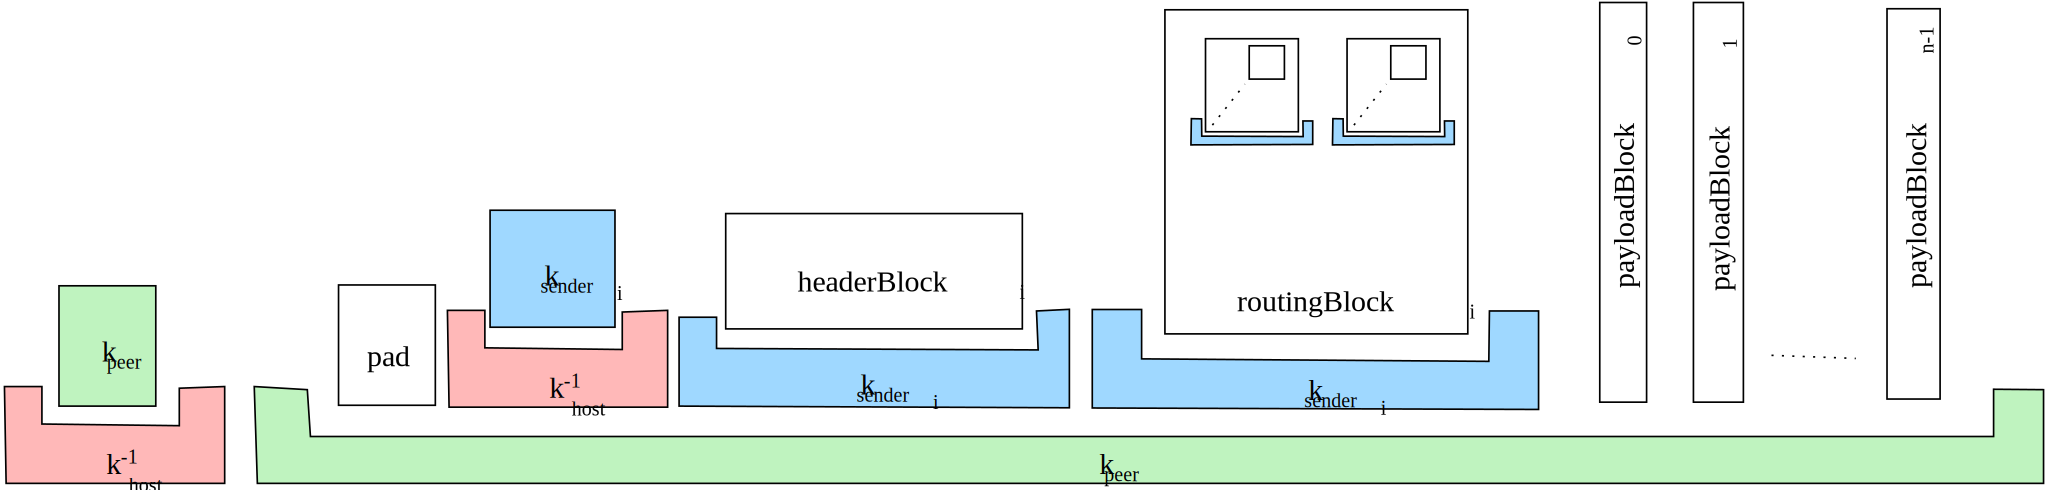
\includegraphics[width=\textwidth]{inc/blockLayoutSimplified}
	$\splitatcommas{\langle \mathbf{MPREFIX_o}, E_{K_{peer_{o+1}}}\left( \mathbf{HPREFIX_o}, \mathbf{HEADER_o}^{K_{sender_o}}, \mathbf{ROUTING_o}^{K_{sender_o}}, payload* \right) \rangle}$
	\caption{Simplified message outline visually and in math}
	\label{fig:messageOutline}
\end{figure}

The first block is the message prefix block $\mathbf{MPREFIX_o}$, which has been encrypted with the public key of the receiving node $K^1_{host_o}$. This block contains the key for decrypting the whole rest of the message. Each PREFIX block contains a symmetrical ey and the specification on how to encrypt or decrypt with it (mode, padding, IV, and other possibly required parameters) in ASN.1 encoding. 

Immediately following the message prefix block, we have the inner message block. This message blocks contain three more blocks and a variable number of payload blocks. The inner message is encrypted with the symmetrical peer key $K_{peer_o}$. This peer key is specific to this message and nowhere reused. It is only known by the two peer hosts $host_o$ and $host_{o-1}$, and the routing block builder (\defref{RBB}). More importantly, $host_{o-1}$ does not need to know the host key of $host_o$. Therefore, relaying a message to $host_o$ does not enable $host_{o-1}$ to communicate with $host_o$. 

The blocks $HEADER_o$ and $ROUTING_o$ are protected with an additional key $K_{sender_o}$. The decryption key is obtained by $host_o$ from the header prefix block $\mathbf{HPREFIX}$. After only decrypting the header block $\mathbf{HEADER}$ and verifying its signature, the accounting layer may check if further processing is authorized. The splitting of the two keys allows us to\ldots
\begin{itemize}
	\item \ldots send a message to $host_o$ without $host_{o-1}$ knowing the host key of $host_o$.
	\item \ldots hide the structure of the message itself.
	\item \ldots keep the content of $\mathbf{HEADER_o}$, and $\mathbf{ROUTING_o}$ secret from $host_{o-1}$.
\end{itemize}

After authorization by the accounting layer, the header block is processed as outlined in section~\ref{sec:processingIncommingMessages}. Basically, we just add the routing blocks and payload to the respective \defref{workspace} and wait for the routing layer to process the information.

Looking at a full \VortexMessage, we get the protocol outline, as shown in \eqref{eq:vortexMessage} on page~\pageref{eq:vortexMessage}.

\begin{figure*}[!ht]
	\begin{align}
	\mathbf{VORTEXMESSAGE}       = &\langle \mathbf{MP}^{K^{-1}_{host_o}}, INNERMESSAGE \rangle \label{eq:vortexMessage} \\ 
	\mathbf{INNERMESSAGE}        = &\langle \mathbf{CP}^{K^{-1}_{host_o}}, \mathbf{H}^{K_{sender_o}}, E^{K^{-1}_{sender_o}}\left(H\left(\mathbf{HEADER}\right)\right), \left[\mathbf{R}^{K_{senderN}}\right], \left[\mathbf{PL}\right]*\rangle^{K_{peerN}} \label{eq:innerMessage}\\
	\mathbf{MP}^{K^{-1}_{hostN}} = &E^{K^{-1}_{hostN}}\left(\mathbf{PREFIX}\langle K_{peerN}\rangle \right)\\ 
	\mathbf{HP}^{K^{-1}_{hostN}} = &E^{K^{-1}_{hostN}}\left(\mathbf{HPREFIX}\langle K_{senderN}\rangle \right)\\ 
	\mathbf{H}^{K_{senderN}}     = &E^{K_{senderN}}\left(\mathbf{HEADER}\right)\\  
	\mathbf{HEADER}              = &\langle K^{1}_{senderN}, serial, maxReplays, validity, [requests, requestRoutingBlock],\nonumber\\ 
	& [puzzleIdentifier, proofOfWork] \rangle \\  
	\mathbf{R}^{K_{senderN}}     = & E^{K_{senderN}}\left(\mathbf{ROUTING}\right)\\ 
	\mathbf{ROUTING}             = & \langle [ \mathbf{ROUTINGCOMBO} ] *, forwardSecret, \mathbf{replyBlock},\mathbf{operations} \rangle\\  
	\mathbf{ROUTINGCOMBO}        = & \langle processIntervall, K_{peerN+1}, recipient, \mathbf{nextMP}, \mathbf{nextHP}, \nonumber \\
	& \mathbf{nextHEADER}, \mathbf{nextROUTING}, \mathbf{assemblyInstructions} \rangle\\
	\mathbf{nextMP}              = & E^{K^1_{host_{o+1}}} \left( K_{peer_{o+1}} \right)\\
	\mathbf{nextHP}              = & E^{K^1_{host_{o+1}}} \left( K_{sender_{o+1}} \right)\\
	\mathbf{nextHEADER}          = & E^{K_{sender_o}} \left( \mathbf{HEADER_{o+1}} \right)\\
	\mathbf{nextROUTING}         = & E^{K_{sender_o}} \left( \mathbf{ROUTING_{o+1}} \right)\\    
	\mathbf{operations}          = & \langle \text{list of operations} \rangle \\
	\mathbf{assembyInstructions} = & \langle  blendingInformation, nextHop, \langle \text{list of mapping operations}\rangle\rangle\\
	\mathbf{PL}                  = &\langle \text{payload octets} \rangle *\\ 
	\end{align}
	%\captionsetup{labelformat=empty}
	\caption{Detailed representation of a VortexMessage}
	\label{fig:mathMessage}
\end{figure*}

The routing log block is an onionized block. It contains at least a $forwardSecret$, which must match up with the header blocks $forwardSecret$. This mechanism is required to guarantee that routing blocks are not exchanged. The $replyBlock$ provides a possibility, if provided, to contact the original sender of the message without knowing him. It is just a routing block with instructions on how to prepare the message to be sent. The routing combos contain all the necessary information and prebuilt blocks to create the subsequent messages.

At the very end, we got the payload. These blocks are simply added to the \defref{eID}s \defref{workspace}.

The double encryption of the routing and header block, are doubly encrypted. We could argue that the inner message block should not be encrypted with a peer key. This looks like a flaw at first sight but is, in fact, a feature that is very important. Without this key, any independent observer with knowledge about the blending capabilities of a receiving node may\ldots
\begin{itemize}
	\item Easier to identify the block structure.\\ 
	This statement remains regardless of whether ASN.1 or length prefixed structures are used. If the structure of a \VortexMessage is easily identified, the messages may be logged or dropped.
	\item Identify the routing block size.\\
	The value of this information is only minimal as it only reflects the complexity of the remaining routing information indirectly.
	\item Identify the number of payload blocks and their respective sizes. \\
	Sizing information is valuable when following the path of a message.
\end{itemize}

\subsubsection{Message Structure Related to Censorship Circumvention}
It is important to note that there is no structure dividing the encrypted peer key from the Inner message block. The size of the peer key block is defined by the key and algorithm of the host key. 

The whole \VortexMessage is, looking from outside, a structureless blob with a maximum of entropy caused by the encryption employed. 

This is intentional and by design. Plain embedding uses furthermore a method of splitting, which allows a message block to be embedded in chunks in carrier information. By design, neither the message nor their embedding display detectable attributes allowing them to identify the message. 

Exactly as with the routing operations, great care has been applied. Any random sequence of bytes may be interpreted as valid chunking. For more exact implementation details on chunking, see section~\ref{sec:chunkingPlain}.

\subsubsection{Message Structure Related to Information Leaking}
From the inside, the $\mathbf{INNERMESSAGE}$ (see \ref{eq:innerMessage}) is built as a structure leaking the absolute minimum of information. A node receiving and decoding the message will learn the following information:
\begin{itemize}
	\item IP of the sender of the transport layer.
	\item The address and embedding schemes of all receiving transport layers.
	\item The size of the payload blocks.
	\item The size of the subsequent routing blocks.
	\item The peer key $K_{peer_o}$.
	\item The size of the prefix blocks.
\end{itemize}

It is unable to extract the following information:
\begin{itemize}
	\item The required keys to communicate with the suspected peer node.
	\item Any information related to message size, content, or recipient.
\end{itemize}

\subsection{Routing Operations\label{sec:operations}}
The routing operations build the core as they define the capabilities of the mixing. We decided to introduce three different classes of operations. Wherever we employ crypto, operations, we may choose the operation required for the operation. No choices exist for the core Reed-Solomon-Function, the padding and spitting operation related to it, and the split and merge operations.

\subsubsection{$addRedundancy$ and $removeRedundancy$ Operations}
I this section we focus on the core operation of our system. The $addRedundancy$ and $removeRedundancy$ allow growing message sizes in our system without allowing to identify the decoy traffic. 

The Lagrange functions have been proposed in \cite{shamir1979share} and further more generalized in \cite{mceliece1981sharing} for sharing secrets. The general idea about all proposed schemes is to distribute informations and restrct access to it so that only if a specified number of shares are captured a secret may be rebulit. Unlike proposed in these papers we do not apply privacy to our protocol by sharing the data among many points. Instead we use lagrange functions to create decoy traffic. By doing so even a creator of traffic is unable to tell message traffic from decoy traffic apart. 

These operations build the core of the routing capabilities of a node. The operation allows an \defref{RBB} to add to a message redundancy information or to rebuild a block from a chosen set of information. 

The operation itself is shown in figure~\ref{fig:addRedundancyOperation}. 
\begin{figure}[ht]\centering
	\includegraphics[width=0.8\columnwidth]{inc/addRedundancyOp}
	\caption{Outline of the addRedundancy operation}
	\label{fig:addRedundancyOperation}
\end{figure}

It may be subdivided into the following operations:
\begin{itemize}
	\item Pad the original message block in such a way, that all resulting blocks are a multiple of the block size of the encrypting cipher.
	\item Apply a Reed Solomon operation in a given GF space with a vanderMonde matrix.
	\item Encrypt all resulting blocks with unpadded, symmetrical encryption.
\end{itemize}

The padding applied in the first step is non-standard padding. The reason for this lies in the properties required by the operation. The presence of standard padding may leak, whether the block has been successfully decrypted or not. Therefore, we created a padding with the following properties:
\begin{itemize}
	\item The padding must not leak whether the rebuild cycle of the operation was successful or not.
	\item Anyone knowing the routing block content and the transmitted message must be able to predict any treated block, including all padding bytes.
	\item The padded content must provide resulting blocks of required size to enable non-padded encryption after the RS operation
	\item The padding must work with any size of padding space.
	\item The padded and encrypted block must not leak an estimate of the original content.
\end{itemize}

The padded block $\mathbf{X}$ is created from a padding value $p$, the unpadded block $\mathbf{M}$ and a series of padding bytes. We build $\mathbf{X}$ for a function $RS_{\text{m of n}}$ (allows adding $m$ redundancy blocks) and an encryption block $\mathbf{M}$ sized $K$ as follows:
\begin{eqnarray}
i          & = & len(\mathbf{M})\\
e          & = & k \cdot n\\
l          & = & \left\lceil\frac{i + 4 + C2 }{e}\right\rceil\cdot e\\
p          & = & i + \left( C1 \cdot l \pmod{\left\lfloor\frac{2^{32}-i}{l}\right\rfloor\cdot l}\right)\\
\mathbf{X} & = & \langle p,\mathbf{M},R_{t}\left(s,l-i-4\right)\rangle
\end{eqnarray}    
The remainder of the input block, up to length $l$, is padded with random data. The random padding data may be specified by RBB though a PRNG spec $t$ and an initial seed value $s$. The message is padded up to size $L$. All resulting, encrypted blocks do not require any padding. This because the initial padding guarantees that all resulting blocks are dividable by the block size of the encrypting function. If not provided by an RBB, an additional parameter $C1$ is chosen as random positive integer and $C2=0$  by the node executing the operation.

To reverse a successful message recovery information of a padded block $\mathbf{X}$, we calculate the original message size by extracting $p$ and doing $len(\mathbf{M})=p \pmod{ len(\mathbf{X})}$.

This padding has many important advantages:
\begin{enumerate}
	\item The padding does not leak if the rebuilding of the original message was successful. Any value in the padding may reflect a valid value.
	\item Since we have a value $C2$, the statement that a message size is within $len(\mathbf{X})<size<(len(\mathbf{X})-k\cdot n)$ is no longer true and any value smaller $len(\mathbf{X})-k\cdot n$ may be correct as well.
	\item An RBB may predict the exact binary image of the padded message when specifying $C1$, $C2$, and $R_{t}(s,)$.
	\item A node knowing the original parameters $C1$, $C2$, and the initial PRNG seed $s$ can detect successful decryption.
\end{enumerate}

Apart from being non-standard padding, the padding has additional downsides:
\begin{itemize}
	\item The padding is inefficient compared to simple paddings such as PKCS\#7
	\item The padding requires an initialized PRNG to generate the padding.
	\item Depending on the chosen parameters, the padding overhead may become significant. 
\end{itemize}

After the padding, the date is ready for the Reed-Solomon part of the operation. We first group the data vector into a matrix $\mathbf{A}$ with $m$ columns to do the operations efficiently. The previous padding guarantees that all columns have a length, which is dividable by the block size of the encryption step applied later.

\begin{eqnarray}
t          & = & n-1\\in bytes
\mathbf{A} & = & vec2mat\left(\mathbf{X},\frac{len\left(\mathbf{X}\right)}{m}\right)\\
\mathbf{V} & = & \left(\begin{matrix}
0^0 & 0^1 & 0^2 & \cdots & 0^{(m-1)} \\
1^0 & 1^1 & 1^2 & \cdots & 1^{(m-1)} \\
2^0 & 2^1 & 2^2 & \cdots & 2^{(m-1)} \\
\vdots & \vdots & \vdots & \ddots & \vdots \\
t^0 & t^1 & t^2 & \cdots & t^{(m-1)}
\end{matrix}\right)\\
\mathbf{P} & = & \mathbf{V}\mathbf{A} \left(GF\left(2^\omega\right)\right)\\
\langle \mathbf{Q_1}, \ldots , \mathbf{Q_n} \rangle & = & row2vec(P)\\
R_i & = & E^{K_i}\left(Q_i\right)
\end{eqnarray}    

We apply the Reed-Solomon function by employing a Vandermonde matrix ($\mathbf{V}$). We build the data matrix ($\mathbf{A}$) by distributing the data into $\frac{len\left(\mathbf{X}\right)}{m}$ columns. This results in a matrix with $m$ rows. Unlike in error-correcting systems, we do not normalize the matrix so that the result of the first blocks is equivalent to the original message. Instead, the error-correcting information is distributed over all resulting blocks ($\mathbf{Q_i}$). Since the entropy of the resulting blocks is lowered as shown in figure~\ref{fig:entropy} and may thus leak an estimate of how a resulting block may have been treated, we added the encryption step to equalize entropy again. The previously introduced padding guarantees that there is no further padding on block-level required. The key used to encrypt the single blocks must not be equivalent. Equivalent keys have the side effect encrypting equal blocks into the same cyphertext. We observed faint but statistically relevant reminders of the unencrypted graphs when treating the same block with the same key and different redundancy parameters.

\subsubsection{$encrypt$ and $decrypt$ Operations}
The encrypt and decrypt operations are essential for the requirement that tagging should not be possible. Unlike the $addRedundancy$ and $removeRedundancy$, the splitting operations do not feature any encryption step after splitting or merging. Reusing a payload block that has only been split or merged would repeat the payload pattern on multiple nodes during transfer. That is why we require to have encryption.

The reason for not building this step into the split and merge function was simple. We needed a separate encryption step to be able to work as an onionizing system, and there were use cases where integrated encryption did not make sense. For further details on this topic, see section~\ref{sec:routingStrategies}.


\subsubsection{$mergePayload$ and $splitPayload$ operation}
The $splitPayload$ operation splits a payload block into two chunks of different or equal sizes. The parameters for this operation are:

\begin{itemize}
	\item source payload block $pb_1$
	\item fraction $f$\\
	A floating-point number which is describing the size of the first chunk. If the fraction is "1.0", then the whole payload is transferred to the second target chunk
\end{itemize}

If $len(pb_1)$ expresses the size of a payloadblock called $pb_1$ in bytes, then the two resulting blocks of the SpitPayload Operation $pb_2$ and $pb_3$ have to follow the following rules:

\begin{eqnarray}
split(f, pb_1) & = &\langle pb_1, pb_2 \rangle\\
pb_1.startsWith(pb_2)\\
pb_1.endsWith(pb_3)\\
len(pb_2) & = & floor(len(pb_1)\cdot f)\\
len(pb_1) & = & len(pb_2) + len(pb_3)
\end{eqnarray}

The $mergePayload$ operation combines two payload blocks into one. The parameters for this operation are:

\begin{itemize}
	\item first source payload block $pb_1$
	\item second source payload block $pb_2$
\end{itemize}

If $len(pb)$ expresses the size of a payloadblock called $pb$ in bytes then resulting block of the MergePayload Operation $pb_3$ have to follow the following rules:

\begin{eqnarray}
merge(pb_1, pb_2) & = & pb_3 \\
pb_3.startsWith(pb_1)\\
pb_3.endsWith(pb_2)\\
len(pb_3) & = & len(pb_1) + len(pb_2)
\end{eqnarray}

Unlike other operations, this operation has no encryption step attached to it. We usually attached an encryption step to remove repeating patterns from the \VortexMessage stream.

It has to be mentioned that this operation tuple has some issues when it comes to floating-point implementations. They are solvable but had to be specified unexpectedly precisely in order to enable a true cross-platform implementation. For more information regarding the issue and exact implementation, see section~\ref{sec:implOperations}.


\section{Summary}
The \MessageVortex{}-Protocol is split into the four layers ``Transport'' (a common internet standard protocol), ``blending'' (extracting and embedding \VortexMessages), ``Routing'' (A layer reassembling messages according to received instruction), and ``Accounting'' (Keeps track of all stored data and discards expired information).

All nodes are realized in decentral devices such as computers or mobile phones. Messages are hidden with either plain embedding or (referred) F5 in the transport layer message. The routing layer processes messages by applying operations to messages. Valid operations are encrypt or decrypt a message chunk, split a message chunk into two parts, merge two parts into one, or add or remove redundancy information. The last operation is the most valuable. This operation allows by employing an extended Reed-Solomon-Operation to add decoy traffic to the message flow without enabling a node to identify such traffic. Furthermore, it allows a sender to send parts of a message through multiple chains of routing nodes to a recipient. Each message itself does not leak the message content since depending on the completing block, any message with appropriate length may be valid.

The routing itself is done in a temporarily allocated storage called ``\defref{workspace}'', which is tied to an ephemeral identity (\defref{eID}) represented by an asymmetric key pair. To get an \defref{eID}, a sender typically solves a crypto puzzle. 

Payloads of \VortexMessages{} are mapped into the \defref{workspace}{} and are assigned a unique \defref{ID}{} within that workspace. The subsequent \defref{routing block}s and their \defref{operation}s are added as well and processed in a time interval defined by the \defref{RBB}.


%!TeX program=pdflatex
%!TeX encoding=utf8
%!TeX spellcheck = en_US
%!TeX root = ../../messageVortex.tex

\partepigraph{No matter how hard you work, someone else is working harder.}{Elon Musk, entrepreneur}
\part{Implementation\label{sec:implementation}}
The implementation differs from the academic model in some details. It is formeost more precise than the academic model. Furthermore, it requires a strict definition of the implementation in order to guarantee the interoperability between different implementations.

This section focuses therefore on the details of the reference implementation.

\chapter{Selection of Algorithms, Encodings, and Protocols}
In this chapter, we choose the following mandatory supported algorithms:
\begin{itemize}
	\item Encoding: ASN.1
	\item Encryption
	\begin{itemize}
		\item AES128/256
		\item Camellia128/256
	\end{itemize}
    \item Modes
    \begin{itemize}
    	\item ECB
    	\item GCM
    \end{itemize}
	\item Paddings
	\begin{itemize}
		\item PKCS\#1
		\item PKCS\#7
	\end{itemize}
	\item MACs
	\begin{itemize}
		\item SHA256/512
		\item RIPE-MD256
	\end{itemize}
	\item PRNG
	\begin{itemize}
		\item mrg32k3a
		\item blumMicali
	\end{itemize}
\end{itemize}

Where security relevant we always choose two independent algorithms. As our protocol has the means of signaling them, we may support additional algorithms without affecting communication while improving the variety of available algorithms.

In the following sections, we emphasize on the choice and the encoding used on the protocol level.

For all algorithms we apply the following criteria:
\begin{itemize}
	\item Always focus on common standards
	\item Focus on interoperability when selecting standards
	\item Focus on efficiency (wherever possible use simple, parallelizable algorithms)
	\item When sensible and possible chose at least two unrelated algorithms (e.g., cryptographic algorithms or MACs)
\end{itemize}

\fxwarning{Sumarize subsections}

\section{Encoding Scheme}
As encoding scheme we specified ASN.1\cite{dis19878824}. It is more compact than the originally selected XML-Standard. It is very common in the fields of telecommunication and encryption (e.g. X509 certificates are represented in ASN.1). To maintain biggestmost interoperability, we choose DER encoding as it has exactly one possible representation for every value. This is especially important when dong signing or solving puzzles in our case.

On the downside ASN-1 encoding is, unlike XML, not human readable. As we hide the messages anyway, we considered this as minor flaw, as we need to have an extracting program anyway to see the content of a message.

\section{Cipher Selection}
In this protocol, a lot of encryption and hashing algorithms have to be used. This choice of these algorithms should be explained. 

We decided to define fixed key sizes for symmetric ciphers as we went with block ciphres. For the asymmetric ciphres we encode the keysize in the parameters as they are due to their differences far more often flexible.

\begin{figure}[ht]
\lstinputlisting[linerange={6-100},language=asn.1,multicols=2]{../../../../application-core-library/src/main/asn/MessageVortex-Ciphers.asn}
\caption{Definition of the structures related to ciphers}
\label{fig:defCiphers}
\end{figure}

From the requirements side, we have to follow the following principle:
First of all, we need a subset of encryption algorithms all implementations may rely on. Defining such a subset guarantees interoperability between all nodes regardless of their origins. 

Secondly, we need to have a spectrum of algorithms in such a manner that it may be (a) enlarged if necessary and (b) there is an alternative if an algorithm (or a mathematical problem class) is broken (so that algorithms may be withdrawn if required without affecting the function in general). 

And third, due to the onion-like design described in this document, asymmetric encryption should be avoided in favor of symmetric encryption to minimize losses due to the key length and the generally higher CPU load opposed by asymmetric keys.

If the algorithm is generally bound to specific key sizes (due to S-Boxes or similar constructs), the key size is incorporated into the definition. If not, the key size is handled as a parameter.

The key sizes have been chosen in such a manner that the key types form tuples of approximately equal strength. The support of Camelia192 and Aes192 has been defined as optional. However, as they are wildly common in implementations, they have already been standardized as they build a possibility to step up security in the future.

Having these criteria for choice, we chose to use the following keys and key sizes:
\begin{itemize}
	\item Symmetric
	\begin{itemize}
		\item AES (key sizes: 128, 192, 256)
		\item Camellia (key sizes: 128, 192, and 256)
	\end{itemize}
	\item Asymmetric
	\begin{itemize}
		\item RSA (key size: 2048, 4096, and 8192)
		\item Named Elliptic Curves
		\begin{itemize}
			\item secp384r1
			\item sect409k1
			\item secp521r1
		\end{itemize}
	\end{itemize}
	\item Hashing
	\begin{itemize}
		\item sha3-256
		\item sha3-384
		\item sha3-512
		\item RIPE-MD160
		\item RIPE-MD256
		\item RIPE-MD320
	\end{itemize}
\end{itemize}

Within the implementation, we assigned algorithms to a security strength level:
\begin{itemize}
	\item LOW\\
	AES128, Camellia128, RSA1024, sha3-256
	\item MEDIUM\\
	AES192, Camellia 192, RSA2048, ECC secp384r1, sha3-256
	\item HIGH\\
	AES256, Camellia256, RSA4096, ECC sect409k1, sha3-384
	\item QUANTUM\\
	AES256, Camellia256, RSA8192, ECC secp521r1, ntru, sha3-512
\end{itemize}

This allows categorizing the used algorithms to a strength. This list, however, should only serve the purpose of selecting algorithms for people without cryptological know-how.

\section{Mode Selections}
We evaluated the most common cipher modes for suitability. For MessageVortex, we focussed on modes that have the properties parallelizable, random access, and do not do authentication. The main focus, besides the characteristics mentioned before, was on the question of whether there is an open implementation available in java, which is reasonably tested.

\begin{figure}[ht]
	\lstinputlisting[linerange={99-112},language=asn.1]{../../../../application-core-library/src/main/asn/MessageVortex-Ciphers.asn}
	\caption{Enumeration definition of modes in ASN.1 with support requirements.}
	\label{fig:defModes}
\end{figure}

Figure~\ref{fig:defModes} shows the selected paddings and their requirement level.

Very important was, that we quite often reencrypt already encrypted content. As a result we had not to exclude algorithms such as ECB.

\begin{itemize}
	\item ECB (Electronic Code Book)\\
	      ECB is the most basic mode. Each block of the cleartext is encrypted on its own. This results in a big flaw: blocks containing the same data will always transform to the same ciphertext. This property makes it possible to see some structures of the plain text when looking at the ciphertext. This solution allows the parallelization of encryption, decryption, and random access while decrypting. Due to these flaws, we rejected this mode.
	\item CBC (Cypher Block Chaining)\\  
	      CBC extends the encryption by xor'ing an initialization vector into the first block before encrypting. For all subsequent blocks, the ciphertext result of the preceding block is taken as xor input. This solution does not allow parallelization of encryption, but decryption may be paralleled, and random access is possible. As another downside, CBC requires a shared initialization vector. As with most IV bound modes, an IV/key pair should not be used twice, which has implications for our protocol.
	\item PCBC (Propagation Cypher Block Chaining)\\
	      CBC extends the encryption by xor'ing, not the ciphertext but a xor result of ciphertext and plaintext. This modification denies parallel decryption and random access compared to CBC.
	\item EAX\\      
	      EAX has been broken in 2012\cite{minematsu2013attacks} and is therefore rejected for our use.
	\item CFB (Cypher Feedback)
	      CFB is specified in \cite{dworkin2001recommendation} and works precisely as CBC with the difference that the plain text is xor'ed and the initialization vector, or the preceding cipher result is encrypted. CFB does not support parallel encryption as the ciphertext input from the preceding operation is required for an encryption round. CFB does, however, allow parallel decryption and random access.
	\item OFB\\
	      \cite{dworkin2001recommendation} specifies OFB and works exactly as CFB except for the fact that not the ciphertext result is taken as feedback but the result of the encryption before xor'ing the plain text. This denies parallel encryption and decryption, as well as random access.
	\item OCB (Offset Codebook Mode)\\
	      This mode was first proposed in \cite{rogaway2003ocb} and later specified in \cite{krovetz-ocb-04}. OCB is specifically designed for AES128, AES192, and AES256. It supports authentication tag lengths of 128, 96, or 64 bits for each specified encryption algorithm. OCB hashes the plaintext of a message with a specialized function $H_{OCB}(\mathbf{M})$. OCB is fully parallelizable due to its internal structure. All blocks except the first and the last can be encrypted or decrypted in parallel.
	\item CTR\\
	      CTR is specified in \cite{lipmaa2000ctr} and is a mixture between OFB and CBC. A nonce concatenated with a counter incrementing on every block is encrypted and then xor'ed with the plain text. This mode allows parallel decryption and encryption, as well as random access. Reusing IV/Key-pairs using CTR is a problem as we might derive the xor'ed product of two messages. This problem only applies where messages are not uniformly random such as in an already encrypted block.
	\item CCM\\
	      Counter with CBC-MAC (CCM) is specified in \cite{RFC3610}. It allows to pad and authenticate encrypted and unencrypted data. It furthermore requires a nonce for its operation. The size of the nonce is dependent on the number of octets in the length field. In the first 16 bytes of the message, the nonce and the message size is stored. For the encryption itself, CTR is used. It shares the same properties as CTR. 
	
	      It allows parallel decryption and encryption as well as random access.
	\item GCM (Galois Counter Mode)\\
	      GCM has been defined in \cite{mcgrew2004galois}, and is related to CTR but has some major differences. The nonce is not used (just the counter starting with value 1). To authenticate the encryption, an authentication token $auth$ is hashed with $H_{GFmult}$ and then xor'ed with the first cipher block. All subsequent cipher blocks are xor'ed with the previous result and then hashed again with $H_{GFmult}$. After the last block the output $o$ is processed  as follows: $H_{GFmult}(o\bigoplus (len(A)||len(B))) \bigoplus E^{K^0}(counter_0)$. As a result, GCM is not parallelizable and does not support random access.
	
	      The mode has been analyzed security-wise in \citeyear{mcgrew2004security} and showed no weaknesses in the analyzed fields \cite{mcgrew2004security}. 
	
	      GCM supports parallel Encryption and decryption. Random access is possible. However, authentication of encryption is not parallelizable. The authentication makes it unsuitable for our purposes. Alternatively, we could use a fixed authentication string.
	\item XTS (XEX-based tweaked-codebook mode with ciphertext stealing)\\
	      This mode is standardized in IEEE 1619-2007 (soon to be superseded). A rough overview of XTS may be found at \cite{Martin2010}. It was developed initially for Disks offering random access and authentication at the same time. 
	\item CMC (CBC-mask-CBC) and EME (ECB-mask-ECB)\\ 
	      In \cite{Halevi:2003} \citeauthor{Halevi:2003} introduces a cipher mode which is extremely costly as it requires two encryptions. CMC is not parallelizable due to the underlying CBC mode, but EME is. 
	\item LRW\\
	      LRW is a tweakable narrow-block cipher mode described in \cite{tschorsch:translayeranon}. This mode shares the same properties as EBC but without the weakness of the same clear text block resulting in the same ciphertext. Similarly to XEX, it requires a tweak instead of an IV.
\end{itemize}

We decided to go with mainly cbc. However, most of the implementations are available and lightweight, we therefore were not as restrictive as ususal when defining a minimal set

\section{Padding selection}
A plain text stream may have any length. Since we always encrypt in blocks of a fixed size, we need a mechanism to indicate how many bytes of the last encrypted block may be safely discarded. 

We have chosen for the paddings outlined in figure~\ref{fig:defPaddings} to be supported.
\begin{figure}[ht]
	\lstinputlisting[linerange={114-121},language=asn.1]{../../../../application-core-library/src/main/asn/MessageVortex-Ciphers.asn}
	\caption{Enumeration definition of paddings in ASN.1 with support requirements.}
	\label{fig:defPaddings}
\end{figure}

\subsection{RSAES-PKCS1-v1\_5 and RSAES-OAEP}
This padding is the older of the paddings standardized for PKCS1. It is basically a prefix of two bytes followed by a padding set of non zero bytes and then terminated by a zero byte and then followed by the message. This padding may give a clue if decryption was successful or not. RSAES-OAEP ist the newer of the two padding standards 

\subsection{PKCS7} 
This padding is the standard used in many places when applying symmetric encryption up to 256 bits key length. The free bytes in the last cipher block indicate the number of bytes being used. This makes this padding very compact. It requires only 1 Byte of functional data at the end of the block. All other bytes are defined but not needed.

\subsection{OAEP with SHA and MGF1 padding} 
This padding is closely related to RSAES-OAEP padding. The hash size is, however, bigger, and thus, the required space for padding is much higher. OAEP with SHA and MGF1 Padding is used in asymmetric encryption only. Due to its size, it is important to note that the payload in the last block shrinks to $keySizeInBits/8-2-MacSize/4$.

In our approach, we have chosen to allow these four paddings. The allowed sha sizes match the allowed mac sizes chosen above. It is important to note that padding costs space at the end of a stream. Since we are always using one block for signing, we have to take care that the chosen signing mac plus the bytes required for padding do not exceed the key size of the asymmetric encryption. While this usually is not a problem for RSA as there are keys 1024+ Bits required, it is an essential problem for ECC algorithms as there are much shorter keys needed to achieve an equivalent strength compared to RSA. 

\subsection{Honorable Mention: AP Padding for $redundancy$ Operations}
We have introduced an additional type of padding not related to these paddings. We required for the $addRedundancy$ the following unique properties. Unfortunately, we were unable to find any padding which matched the following properties simultaneously:

\begin{itemize}
	\item Padding must not leak successful decryption\\
	      For our $addRedundancy$ operation, we required padding that had no detectable structure as a node should not be able to tell whether a $removeRedundancy$ operation did generate content or decoy. 
	\item Padding of more than one block\\
	Due to the nature of the operation, it is required to be able to pad more than just one block.
\end{itemize}

This padding is the only padding for the $addRedundancy$ and $removeRedundancy$ operations.

\subsection{Pseudo Random Number Generator Selection\label{sec:prng}}
For our $addRedundancy$ and $removeRedundancy$ operations we needed a pseudo random number generator (PRNG). For our implementation we did not research deeply this part as it seemed irrelevant. The only criteriion was, that it had to create content indistinguishable from an encrypted message. This criterion arose as we use it for padding invisibly an already encrypted message.

The PRNG used for our implementation is an xorshift+ generator. It is based on the XSadd PRNG\cite{marsaglia2003xorshift} and passes the bigcrush PRNG test suite. It is a fast, xor based PRNG which has two internal 64 bit seed states $s_0$ respectively $s_1$ and is defined as follows:

\begin{eqnarray}
x & = & s_0\\
s_0 & = & s_1\\
x & = & x \oplus ( x \ll 23 )\\
s_1 & = & x \oplus s_1 \oplus ( x \gg 17 ) \oplus (s_1 \gg 26 )\\
nextNumber & = & s_1+s_0
\end{eqnarray}

We have chosen this comparably weak PRNG for practical reasons. It is fast, simple, and is based on operations easy to implement on hardware. As we do not need a cryptographically strong PRNG, it is our primary choice so far. 

As the protocol is heavily dependent on security we have introduced everywhere at least one alternate algorithm which may be used if one of the choices may become a problem. In order to have a second choice for the PRNG we define the Blum-Micali PRNG as described in \cite{blum1984generate}. This PRNG is a cryptographically secure PRNG and is defined as follows:

$p$ is prime and $g$ is a primitive root modulo $p$. $x_0$ reflects the seed state.

\begin{eqnarray}
x_{i+1}=g^{x_i}\mod p
\end{eqnarray}

%\subsection{Puzzle Selection}
%\fxwarning{Add content here... maybe old text about PoW-Algorithms}
% Erradicated old text too inocomplete and massive work required

\section{Transport Layer Protocol Selection}
The following sections list common Internet protocols. We analyze those protocols for the fitness as transport layer of message vortex. 

We will identify SMTP and XMPP as good transport layer protocols for the \MessageVortex approach, as they have all required properties.

All sections are structured the same way. We first refer to the protocol or standard and describe it in the simplest possible form. We refer to subsequent standards if required to consider extensions where sensible. We then apply the previously referenced criteria and make a concise summary of the suiting of the protocol as a transport layer. The findings of this section is listed in table \ref{tab:protoSuitCrit}. The list here does not reflect the quality or maturity of the protocols. It is a simple analysis of suiting as a transport layer.

All sections are structured the same way. 
\begin{itemize}
	\item Description\\
	We first refer to the protocol or standard and describe it in the simplest possible form. We refer to subsequent standards if required to consider extensions where sensible.
	\item Apply criteria\\\\
	We then apply the previously referenced criteria and make a concise summary of the suiting of the protocol as a transport layer. The findings of this section is listed in table \ref{tab:protoSuitCrit}. The list here does not reflect the quality or maturity of the protocols. It is a simple analysis of suiting as a transport layer.
\end{itemize} 

\subsection{Applied Criteria\label{sec:transportCriteria}}
\begin{itemize}
	\item Widely adopted (Ct1)\\
	The more widely adopted and used a protocol is, the harder it is due to the sheer mass for an adversary to monitor , filter, or block the protocol. This is important for censorship resistance of the protocol. 
	\item Reliable (Ct2)\\
	Message transport between peers should be reliable. As messages may arrive anytime from everywhere, we do not have means to synchronize the peer partners on a higher level without investing a considerable effort. Furthermore, the availability of information when what type of information should be available at a specific point in the system would drastically simplify the identification of peers. To avoid synchronization, we do look for inherently reliable protocols.
	\item Symmetrical built (Ct3)\\
	The transport layer should rely on a peer to peer base. All servers implement a generic routing that requires no prior knowledge of all possible targets. This criterion neglects centralized infrastructures. This criterion may be dropped, assuming that the blending layer or a specialized transport overlay is responsible for routing.
\end{itemize}

\subsection{Analyzed Protocols}
We were unable to find a comprehensive list of protocols being used within the Internet and their bandwidth consumption. A weak reference is \cite{zhou2011examining}. This wekaness is founded in the fact that traffic in this report is callified among two critera: Know server or known port. As streaming services consume a considerable part of the Internet bandwidth (acording to the report more than 60\% download). The focus on the report lies on the bandwidth intense figures. However, leavin aside all sources which are strictly one way or dominated by a small number of companies worldwide, the ``top 10'' list of the report shrinks to the two categories ``File sharing'' (Rank 5; 4.2\% download and 30.2\% upload) and ``Messaging'' (Rank 8; 1.6\% download and 8.3\% upload bandwidth). 

In lack of such material we first collected a list of all common Internet messaging protocols (synchronous and asynchronous). We added furthermore some of the most common transfer protocols such as HTTP and FTP and analyzed this list.

\begin{itemize}
	\item Messaging Protocols
	\begin{itemize}
		\item SMTP
		\item CoAP
		\item MQTT
		\item AMQP
		\item XMPP
		\item WAMP
		\item SMS
		\item MMS
	\end{itemize}
	\item Other Protocols
	\begin{itemize}
		\item FTP, SFTP, and FTPS
		\item TFTP
		\item HTTP
	\end{itemize}
\end{itemize}

The following protocols have been discarded as we have considered them as outdated:
\begin{itemize}
	\item MTP\cite{RFC780} (obsoleted by SMTP)
	\item NNTP\cite{RFC3977} (outdated and has only a small usage acording to \cite{kim2010today})
\end{itemize}

We furthermore discarded all RPC-related protocols as they would by definition violate Ct3.

\subsection{Analysis}
\subsubsection{HTTP}
The HTTP protocol allows message transfer from and to a server and is specified in RFC2616 \cite{rfc2616}. It is not suitable as a communication protocol for messages due to the lack of notifications. There are some extensions that would allow such communications (such as WebDAV). Still, in general, even those are not suitable as they require a continuous connection to the server to get notifications. Having a ``rollup'' of notifications when connecting is not there by default but could be implemented on top of it. HTTP servers listen on standard ports 80 or 443 for incoming connects. The port 443 is equivalent to the port 80 except for the fact that it has a wrapping encryption layer (usually TLS). The incoming connects (requests) must offer a header part and may contain a body part that would be suitable for transferring messages to the server. The reply to this request is transferred over the same TCP connection containing the same two sections.

HTTP0.9-HTTP/1.1 are clear text protocols which are human-readable (except for the data part which might contain binary data). The HTTP/2\cite{rfc7540} protocol is using the same ports and default behavior. Unlike HTTP/0.9-HTTP/1.1, it is not a clear text but encodes headers and bodies in binary form. 

To be a valid candidate as storage, unauthenticated WebDAV support, as specified in \cite{rfc4918}, must be assumed.

The protocol does satisfy the first two main criteria (Ct1: Widely Adopted and Ct2: Reliable). The main disadvantage in terms of a message transport protocol is that this protocol is not symmetrically. A server is always just ``serving requests'' and not sending information actively to peers. This Request-Reply violates criteria (Ct3: Symmetrically built) and makes the protocol not a primary choice for message transport. 

It is possible to add such behavior to the blending layer using HTTP servers as pure storage. Such a behavior would however be most likely detectable and thus no longer be censorship resistant.

\subsubsection{FTP}
FTP is defined in RFC959\cite{RFC959}. This Protocol is intended for authenticated file transfer only. There is an account available for general access (``anonymous''). This account does normally not offer upload rights for security reasons. It is possible to use FTP as a message transfer endpoint. The configuration would work as follows: the user ``anonymous'' has upload rights only. It is unable to download or list a directory. A node may upload a message with a random name. In case a collision arises, the node retries with another random name. The blending layer picks messages up using an authenticated user. This workaround has multiple downsides. At first, handling FTP that way is very uncommon and usually requires an own dedicated infrastructure. Such beavior would make the protocol again possibly detectable. Secondly, passwords are always sent in the clear within FTP. Encryption as a wrapping layer (FTPS) is not common, and SFTP (actually a subsystem of SSH) has nothing in common with FTP except for the fact that it may transfer files as well.

Furthermore, FTP may be problematic when used in active mode for firewalls. All these problems make FTP not very suitable as a transport layer protocol. FTPS and SFTP feature similar weaknesses as the FTP version in terms of detectability of non-standard behavior.

Like in HTTP, a disadvantage of FTP in terms of a message transport protocol is that this protocol is not symmetrically. A server is always just ``serving requests'' and not sending information actively to peers. This Request-Reply violates criteria (Ct3: Symmetrically built) and makes the protocol not a primary choice for message transport. The Protocol, however, satisfies the first two criteria  (Ct1: Widely Adopted and Ct2: Reliable).

\subsubsection{TFTP}
TFTP has, despite its naming similarities to FTP, very little in common with it. TFTP is a UDP based file transfer protocol without any authentication scheme. The possibility of unauthenticated message access makes it not suitable as a transport layer. The protocol is due to the use of UDP in a meshed network with redundant routes. Since the Internet has a lot of these redundant routes, this neglects the use of this protocol.

TFTP is rarely ever used on the Internet, as its UDP based nature is not suitable for a network with redundant routes. Not being common on the Internet violates criterion one (Ct1: Widely Adopted). TFTP is not symmetrically. This means that a server is always just ``serving requests'' and not sending information actively to peers. This Request-Reply violates criteria (Ct3: Symmetrically built) and makes the protocol not a primary choice for message transport. The Protocol furthermore violates Ct2 (Ct2: Reliable) as it is based on UDP without any additional error correction.

\subsubsection{MQTT}
MQTT is an ISO standard (ISO/IEC PRF 20922:2016) and was formerly called MQ Telemetry Transport. The current standard as the time of writing this document was 3.1.1 \cite{mqtt}. 

The protocol runs by default on the two ports 1883 and 8883 and can be encrypted with TLS. MQTT is a publish/subscribe based message-passing protocol that is mainly targeted to m2m communication. This Protocol requires the receiving party to be subscribed to a central infrastructure in order to be able to receive messages. This makes it very hard to be used in a system without centralistic infrastructure and having no static routes between senders and recipients. 

The protocol does satisfy the second criterion (Ct2: Reliable). It is in the area of end-user (i.e., Internet) not widely adopted, thus violating Criteria 1 (Ct1: Widely Adopted). In terms of decentralization design, the protocol fails as well (Ct3: Symmetrically built).

\subsubsection{Advanced Message Queuing Protocol (AMQP)}
The Advanced Message Queuing Protocol (AMQP) was initially initiated by numerous exponents based mainly on finance-related industries. The AMQP-Protocol is either used for communication between two message brokers, or between a message broker and a client\cite{amqp}.

It is designed to be interoperable, stable, reliable, and safe. It supports either SASL or TLS secured communication. The use of such a tunnel is controlled by the immediate sender of a message. In its current version 1.0, it does, however, not support a dynamic routing between brokers\cite{amqp}.

Due to the lack of a generic routing capability, this protocol is therefore not suitable for message transport in a generic, global environment.

The protocol satisfies partially the first criterion (Ct1: Widely Adopted) and fully meets the second criterion (Ct2: Reliable). However, the third criterion is violated due to the lack of routing capabilities between message brokers (Ct3: Symmetrically built).

\subsubsection{Constrained Application Protocol (CoAP)}
The Constrained Application Protocol (CoAP) is a communication Protocol which is primarily destined to m2m communication. It is defined in RFC7252\cite{RFC7252}.  It is defined as a lightweight replacement for HTTP in IoT devices and is based on UDP.

The protocol does partially satisfy the first criteria (Ct1: Widely Adopted). The second criterion (Ct2: Reliable) is only partially fulfilled as it is based on UDP and does only add limited session control on its own.

The main disadvantage in terms of a message transport protocol is that this protocol is not (like HTTP) symmetrically. This means that a server is always just ``serving requests'' and not sending information actively to peers. This Request-Reply violates criteria (Ct3: Symmetrically built) and makes the protocol not a primary choice for message transport. 

\subsubsection{Web Application Messaging Protocol (WAMP)}
WAMP is a web-sockets based protocol destined to enable M2M communication. Like MQTT, it is publish respectively subscribe oriented. Unlike MQTT, it allows remote procedure calls (RPC).

The WAMP protocol is not widely adopted (Ct1: Widely Adopted), but it is reliable on a per-node base (Ct2: Reliable). Due to its RPC based capability, unlike MQTT, a routing like capability could be implemented. Symmetrical protocol behavior is therefore not available but could be built in relatively easy.

\subsubsection{XMPP (jabber)}
XMPP (originally named Jabber) is a synchronous message protocol used in the Internet. It is specified in the documents RFC6120\cite{RFC6120}, RFC6121\cite{RFC6120}, RFC3922\cite{RFC3922}, and RFC3923\cite{RFC3923}. The protocol is a very advanced chat protocol featuring numeros levels of security including end-to-end signing and object encryption\cite{RFC3923}. There is also a stream initiation extension for transferring files between endpoints \cite{xep0096}.

It has generic routing capabilities spanning between known and unknown servers. The protocol offers a message retrieval mechanism for offline messages similarily to POP \cite{xep0013}.

The protocol itself seems to be a strong candidate as a transport layer as it is being used actively on the Internet.

\subsubsection{SMTP}
The SMTP protocol is currently specified in \cite{RFC5321}. It specifies a method to deliver reliably asynchronous mail objects through a specific transport medium (most of the time, the Internet). The document splits a mail object into a mail envelope and its content. The envelope contains the routing information, which is the sender (one) and the recipient (one or more) in 7-Bit ASCII. The envelope may additionally contain optional protocol extension material. 

The content should be in 7-Bit-ASCII (8-Bit ASCII may be requested, but this feature is not widely adopted). It is split into two parts. These parts are the header (which does contain meta-information about the message such as subject, reply address, or a comprehensive list of all recipients), and the body which includes the message itself. All lines of the content must be terminated with a CRLF and must not be longer than 998 characters, excluding CRLF.

The header consists of a collection of header fields. Each of them is built by a header name, a colon, and the data. The exact outline of the header is specified in \cite{RFC5322} and is separated with a blank line from the body. 

\cite{RFC5321} furthermore introduces a simplistic model for SMTP message-based communication. A more comprehensive model is presented in section \nameref{sec:mailTransport} as the proposed model is not sufficient for a detailed end-to-end analysis.

Traditionally the message itself is mime encoded. The MIME messages are mainly specified in \cite{RFC2045} and \cite{RFC2046}. MIME allows to send messages in multiple representations (alternates), and attach additional information (such as possibly inlined images or attached documents). 

SMTP is one of the most common messaging protocols on the Internet (Ct1: Widely Adopted), and it would be devastating for the business of a country if, for censoring reasons, this protocol would be cut off. The protocol is furthermore very reliable as it has built-in support for redundancy and a thorough message design making it relatively easy to diagnose problems (Ct2: Reliable). All SMTP servers usually are capable of routing and receiving messages. Messages going over several servers are common (Ct3: Symmetrically built), so the third criterion may be considered as fulfilled as well.

SMTP is considered a strong candidate as a transport layer.  

\subsubsection{SMS and MMS}
SMS capability was introduced in the SS7 protocol. This protocol allows the message transfer of messages not bigger than 144 characters. Due to this restriction in size, it is unlikely to be suitable for this type of communication as the keys being required are already sized similarly, leaving no space for Messages or routing information.

The \nth{3} Generation Partnership Project (3GPP) maintains the Multimedia Messaging Service (MMS). This protocol is mainly a mobile protocol based on telephone networks.

Both protocols are not widely adopted within the Internet domain. There are gateways providing bridging functionalities to the SMS/MMS services. However, the protocol itself is insignificant on the Internet itself. 

\subsubsection{MMS}
This protocol is just like the SMS protocol accessible through the Internet by using gateways but not directly usable within the Internet.

\subsection{Results}
We have shown that all common M2M protocols failed mainly at Ct3 as there is no need for message routing. In M2M communication contacting foreign machines is not common. Therefore M2M protocolls are typically using static M2M communication over prepared channels. Such behavior is, however unsuitable for a generic messaging protocol.

Pure storage protocols fail at the same criteria as they typically have a defined set of data sources and data sinks, whereas usually at least the data sources are limited in number. This makes those protocols unsuitable again.

We can clearly state that according to the criteria, only a few protocols are suitable. Table \ref{tab:protoSuitCrit2} on page \pageref{tab:protoSuitCrit} shows that only SMTP and XMPP are suitable protocols. Eventually, similar protocols such as HTTP (with WebDAV) or FTP may be usable as well. 

\begin{table}[h]
	\centering\tiny
	\begin{tabular}{|l|l|l|l|}\hline
		\diaghead{\theadfont protocol Criteria}{Protocol}{Criteria} & \thead{Ct1: Widely adopted}     & \thead{Ct2: Reliable} & \thead{Ct3: Symmetrically built}\\\hline
		HTTP     & $\checkmark$            & $\checkmark$        & $\times$\\              
		FTP      & $\checkmark$            & $\checkmark$        & $\times$\\
		TFTP     & $\times$                & $\times$            & $\times$\\
		MQTT     & \textasciitilde         & $\checkmark$        & $\times$\\              
		AMQP     & \textasciitilde         & $\checkmark$        & $\times$\\
		CoAP     & \textasciitilde         & \textasciitilde     & $\times$\\
		WAMP     & $\times$                & $\checkmark$        & \textasciitilde\\
		XMPP     & $\checkmark$            & $\checkmark$        & $\checkmark$\\
		SMTP     & $\checkmark$            & $\checkmark$        & $\checkmark$\\\hline
	\end{tabular}    
	\caption{comparison of protocols in terms of the suitability as transport layer}
	\label{tab:protoSuitCrit2}
\end{table}

The findings of this short analysis suggested that we should use the two protocols, SMTP and XMPP, for our first standardization. We require at least two to prove that the protocol is agnostic to the transport.

\chapter{Transport Layer Implementation}
\section{Implementation of a Dummy Transport Layer}
For better diagnosability and fast setup, we implemented a custom transport layer working on a config-less manner in a localhost or broadcast-domain environment. The transport layer is based on the Hazelcast distributed hashmap. Implementation may be found under \lstinline[columns=fixed]{net.messagevortex.transport.dummy.DummyTransportTrx}. 

\section{Implementation of an Email Transport Layer}
Email supports a conglomerate of protocols. Looking at the client side, we will find that email is sent with an authenticated SMTP connection. The SMTP connection is somewhat different than than the connections used to send emails to the destination. First of all the client port was shifted in the past to a specific submission port (SMTPS: Port 465; Submission: Port 587). These submmission ports are authenticated (either by username and password, by IP or by certificates) and usually privileged (no \defref{UBE} checks). On the retrieval side, SMTP is not capable of handling these tasks sensibly. Instead, POP3 and IMAPv4 are used. POP3 is a deposit box for email where a device fetches the mail and stores it locally. This is commonly in use for automated processing of mails but these days, where the same user owns multiple devices no longer adequate. IMAPv4 offers to organize mails on the server. This allows a user to have the same folder structure of mails in a synchronized manner on all devices.

For an ideal implementation we would do the following: Organize our \MessageVortex{} mails in a separate account. The account is accessed through a local proxy relaying our ``ordinary outgoing mails'' through the SMTP server of our regular provider and all \MessageVortex{} related traffic through the provider of our \MessageVortex{} mailbox. Keeping the two mailboxes separate is sensible and important as we will see in part~\ref{sec:operation}. The housekeeping on the account used for \MessageVortex{} is done automatically and in a sensible way, comparable to a human (e.g., handle draft, sent and trash bin folders sensibly and keep all mails in a flat structure deleting old mails from time to time). The mails from the regular and the \MessageVortex{} account are merged by the proxy in a transparent way. Keeping the messages apart but offering a unified look.

In our current implementation the house keeping part has been skipped. Instead, we are just fetching the newly arrived messages and put in a local storage. The email presented to the client is provided by a local IMAP server. Persistence of these messages is not yet implemented. 

\section{Implementation of an XMPP Transport Layer}
The XMPP protocol (formerly called  Jabber, as specified in \cite{RFC6120}, is natively not capable of transferring anything else but text messages. Unlike email, XMPP is capable of true end-to-end signing and object encryption without solving the problem of the initial trust. While we may use the end-to-end encryption for additional security, relying on this feature is not sensible as we would put trust into the security features of an intermediate node. This would effectively violate \ref{req:zeroTrust} requirement. We decided to use the extension defined in \cite{xep0231} to transfer our messages, as it is simple and reliable.

To transfer a \VortexMessage{}, we could embedd a MIME message just as with  SMTP. While this would be technically feasible, the usage of MIME is not common and even discouraged. Instead, the inner structure if an XMPP message relies on XML. 

XMPP has an improvment process based on XEPs. For including binary contents such as attachments in messages multiple XEPs exists. Table~\ref{tab:xep} shows all idenified candidates.
\begin{table*}[ht]\centering\tiny
	\label{tab:xep}
	%\setlength{\aboverulesep}{0pt}
	%\setlength{\belowrulesep}{0pt}
	\newcolumntype{x}[1]{!{\centering\arraybackslash\vrule width #1}}
	\rowcolors{2}{black!30}{black!10}
	\bgroup
	\def\arraystretch{1.5}%  1 is the default, change whatever you need
\begin{tabular}{|l|l|p{8cm}|}\hline
	Name                                 & Status (as of 06-2020)             & Purpose \\\hline
	\citetitle{xep0047}\cite{xep0047}    & Final Standard                     & Allows sending chunked, base64 encoded data within the jabber connections.\\
	\citetitle{xep0066}\cite{xep0066}    & Draft Standard                     & Allows sending URIs of remotely hosted binary data.\\
	\citetitle{xep0096}\cite{xep0096}    & Depreciated (referred to XEP-0234) & Improvement of \cite{xep0066} allowing to send metadata and alternative URIs\\
	\citetitle{xep0135}\cite{xep0135}    & Deferred (inactive)                & Inband or Out-of-band file discovery and referral service. May be used in conjunction with FTP, HTTP, SCP, or \cite{xep0096}.\\
	\citetitle{xep0231}\cite{xep0231}    & Draft Standard                     & Allows sending inband small unchunked files and referring within the message similarly to \cite{rfc2397}.\\
	\citetitle{xep0234}\cite{xep0234}    & Deferred (inactive)                & Based on \cite{xep0166} allowing out-of-band content negotiation of complex data streams\\\hline 
\end{tabular}
\caption{Overview of XEPs related to transporting binary data.}
\egroup
\end{table*}

Many documents have either reached standard or have been deferred due to inactivity.  We used ``\citetitle{xep0231}''\cite{xep0231} for our protocol. It is simple to implement as a transport layer, used in many clients (e.g., Prosody, Pigdin, or CoyIM). A node may use any XMPP server regardless of any additional support for transfer.

The blending layer may generate decoy message analogue to the messages generated in the case of email.

\section{Distributed Configuration and Runtime Store of processing content}
If we care to run our \MessageVortex nodes in a sensible and 

\chapter{Blending Layer Implementation}
\section{Embedding Spec}
We always embed VortexMessages as attachments in SMTP and XMPP messages. 

The embedding supports some properties. A receiving host chooses the supported properties. We describe valid properties by the blending specification in EBNF as follows:
\begin{lstlisting}[language=EBNF]
plainEmbedding = "("plain:"<#BytesOffset>[,<#BytesOffset>]*")
F5Embedding    = "(F5:"<passwordString>[,<PasswordString>]*")"
\end{lstlisting}

\fxwarning{ Story: Both embeddings allow unbroken logical structure (plain->generic and F5 for JPEG/GIF/BMP). When advertizing multiple offsets or PWs then all of them are checked by blending layer. Presence of a valid header block is sufficient proof.}



\subsection{Plain Embedding}
The $plainEmbedding$ is a simple embedding replacing parts of the original file with the content of the \VortexMessage. To maintain the header information of a file we introduced an offset as a set of fixed values. A plain embedding may be identified by a host when decoding a single block with $K^{-1}_{host_o}$ if the resulting structure is an ASN.1 stucture is equivalent to XXX.


We use mainly plain embedding for our experiments. For better readability, we used a specialized blending layer using unchunked, plain embedding with an offset of $0$. The message itself was the ASN.1 block representation of the encoded block. The chosen encoding simplified to see the inner workings of the protocol. For production use, we apply F5 embedding with a generated payload. The current implementation of the blending layer employing plain embedding is thus not suitable for production use as the messages remain identifiable or at least suspicious.

\subsubsection{Chunking of Plain Embedded Messages}\label{sec:chunkingPlain}
In this section we describe the chunked embedding into plain messages. The chunking is done by embedding one to four byte integer values which reflect (modulo the the remaining file size) the next chunk and the following gap. The byte layout is chosen in such a way that any byte sequence from two to eight bytes form a valid chunk header.

When plain embedding messages we have the problem that most of the files have recurring logical structures. Such structures should not be broken when embedding in plain as such embedding as it would leak in an easy detectable manner the presence of a broken file.



\subsection{Implementation of F5 Blending}
\fxwarning{complete section with story "Implementation of F5 Blending"}
\fxwarning{Story: F5 \cite{f5} is very old and has not been broken. The first implementation had a detectable issue with an unintended double compression \cite{steganalysisf5} but the authors of f5 fixed this issue \cite{F5broken}. newer derivates and alternatives are available (e.g., nsF5 or   MSET)}

\section{Blending Content Generation}
\fxwarning{complete section}

\chapter{Routing Layer Implementation}
\fxwarning{complete section}
\section{ASN.1 encoding scheme}
Originally, we implemented the protocol as XML encoded messages. This encoding had, however, several flaws. First the huge ammount of encrypted data within the document made the messages bulky and at the same time loose one of its main strengths: readability for humans. The encoding required for binary data caused messages to increase ion size due to their onionized structure. 

Furthermore, the complex XML features \fxwarning{incomplete section}

\section{Processing of messages}
\fxwarning{complete section}

\subsection{Processing of Incoming Messages}\label{sec:processingIncommingMessages}
A Block is picked up in the blending layer and then handled in the routing layer. First, we try to authenticate the message. If we can authenticate the message, we process it and add the contained instructions to a processing workspace. Unauthenticated messages may be discarded at any point.

The processing of a sending block is triggered by a routing block in the workspace, as shown in figure~\ref{fig:msgSendProcessing}. The assembly instructions are processed to collect the payload blocks. Then the encryption is applied to the message and passed on to the blending layer for processing.

\begin{figure*}[hbt]
	\includegraphics[width=0.90\textwidth]{inc/flowchart_message_sending}
	\caption{flow diagram showing processing of outgoing messages}
	\label{fig:msgSendProcessing}
\end{figure*}

\fxwarning{complete section}

\subsection{Processing of Outgoing Messages}\label{sec:processingOutgoingMessages}
\fxwarning{complete section}

\subsection{Implementation of Operations}\label{sec:implOperations}
\fxwarning{Mention mapping operation}

\fxwarning{Mention floating point issues when splitting}

\fxwarning{complete section}

\section{Request handling}
\fxwarning{complete section}

\subsection{Requesting a new Ephemeral Identity}\label{sec:newEID}
\fxwarning{complete section}

\subsection{Replacing an Existing Node Identity}
\fxwarning{complete section}

\subsection{Replacing an Existing Reply Block}\label{sec:replaceMURB}
\fxwarning{complete section}


\chapter{Accounting Layer Implementation}
\fxwarning{complete section}

\chapter{Usability Related Implementation Details}
\fxwarning{complete section}

\section{Adressing and address representations}
\fxwarning{complete section}

\section{Linking to Common User Agents}
\fxwarning{complete section}

\chapter{Efficiency Related Implementation Details}
\fxwarning{complete section}

\section{Node Storage Management}
\fxwarning{complete section}

\subsection{Life-cycle of Ephemeral Identities and Workspaces}
\fxwarning{complete section}

\subsection{Life-cycle of Requests}
\fxwarning{complete section}

\subsection{Life-cycle of Operations}
\fxwarning{complete section}

\section{Overhead Minimization in Message}
\fxwarning{complete section}



%!TeX program=pdflatex
%!TeX encoding=utf8
%!TeX spellcheck = en_US
%!TeX root = ../../messageVortex.tex
\partepigraph{Occurrences in this domain are beyond the reach of exact prediction because of the variety of factors in operation, not because of any lack of order in nature.}{Albert Einstein}
\part{Operational concerns}\label{sec:operation}

\chapter{General Concerns Regarding Operation}
\section{Hardware}
We require no specialized hardware for running Vortex nodes. Instead, we designed Vortex in such a way that ordinary mobile phones may act as Vortex nodes. It is, however, recommended to have a node always connected to the Internet. A mobile phone may disconnect from time to time based on the availability of the network. For our experiments, we used a RaspberryPi Zero W. It is, however, recommended to use a faster, newer model due to the memory requirements of the proof of work algorithm. 

The hardware currently requires a network interface and a fully functional JSE VM to run the reference implementation.

\section{Addressing of Vortex Nodes}
From the start, we were looking for an addressing scheme suitable for transparent addressing.

A Vortex address is built as follows: 

\begin{lstlisting}[language=EBNF]
localPart         = <local part of address>
domain            = <domain part of address>
email             = localPart "@" domain
keySpec           = <BASE64 encoded AsymmetricKey [DER encoded]>
smtpAlternateSpec = localPart ".." [ keySpec ] ".." domain "@localhost"
smtpUrl           = "vortexsmtp://" smtpAlternateSpec
\end{lstlisting}

To allow storage of Vortex addresses in standard messaging programs such as Outlook or Thunderbird, we introduced $smtpAlternateSpec$. 

The suffix ``@localhost'' makes sure that any non-participating server does not route a \VortexMessage{} unintentionally. The doubly dotted notation is not RFC compliant but was accepted by all tested client address books. The address is, however, not a valid SMTP address due to its double-dotted notation. We selected this representation to differentiate Vortex addresses from valid email addresses.

The main downside of vortex addresses is that they are no longer readable by a human. The main reason for this is the public key, which is required. We may abstract this further by allowing clear-text requests on the primary email address for the public key. The vortex account must then answer such requests with the valid Vortex address.

The $smtpUrl$ is representing the address in a standard way, which makes it suitable for QR codes and intent filters on Android.

The public key of an address is encoded as follows:
\begin{enumerate}
	\item The asymmetric key is encoded as specified in the \texttt{AsymmetricKey} in ASN.1
	\item The ASN.1 DER representation is then encoded using BASE64
\end{enumerate}    

The \texttt{keySpec} may be omitted and inserted later from an address list. The quad-dotted resulting address is illegal in a standard mail system and offers a possibility for identification. Such a key-less address may furthermore be used as a synonym for the receivers' real address as any potential receiver may send an unsolicited \texttt{HeaderRequestReplaceIdentity}.

\section{Client}
We did not create a Vortex client for sending messages. Instead, we used a standard Thunderbird email client pointing to a local SMTP and IMAP Server provided by a Vortex proxy. On the SMTP side, Vortex does encapsulate where possible mails into a Vortex message and builds an automated route to the recipient. The SMTP part of Vortex may be used to encapsulate all messages automatically with a known Vortex identity into a \emph{VortexMessage}. On the IMAP side, it merges a local Vortex message store with the standard Email repository building a combined view.

Using Vortex like this offers us the advantages of a known client with the anonymity Vortex offers.

Using a proxy has certain downsides. At the moment, the vortex client has only a local store. Such a local store makes it impossible to handle multiple simultaneously connected clients to use Vortex. This limitation is, however, just a lack of the current implementation and not of the protocol itself. We may safely use IMAP storage for storing \emph{VortexMessages} centrally. This statement is true as long as:
\begin{itemize}
	\item The storage is not identifiable as such.\\
	This requires:
	\begin{itemize}
		\item A non-identifiable folder/message structure
		\item A storage not identifiable by access patterns
		\item The stored messages do have the same strength as the transmitted messages in terms of detectability
	\end{itemize}
	\item A secured key\\
	Either the host key is secured sufficiently with KDF, and a passphrase (or similar), or the host key remains off-storage.
\end{itemize}

\subsection{Vortex Accounts}
By definition, any transport layer address may represent a Vortex identity. This fact may make people believe that their current email or jabber address is suitable as a Vortex address. This statement is technically perfectly true, but should not be done for the following reasons:
\begin{itemize}
	\item If an address is identified as a Vortex address, it may be blocked (directly or indirectly) by an adversary. Such blocking would lead to blocking of regular email traffic as well.
	\item If a vortex node is malfunctioning, non-\emph{VortexMessages} should remain unaffected. Isolation is far better if we keep non-Vortex messages in a separate account.
	\item If a user wants no longer to maintain its Vortex address, he may give up his Vortex transport accounts. If he had been using his normal messaging account for Vortex, he would receive mixing messages which are hard to filter even with a known host key.
\end{itemize}

\subsection{Vortex Node Types}\label{sec:vortexNodeTypes}
Depending on the type of adversary within a jurisdiction, a \VortexNode{} may require different properties. In section~\ref{sec:adversary}, we defined observing and censoring adversaries. In environments with an observing adversary, the presence of a vortex node is not something that we have to keep hidden. In jurisdictions with a censoring adversary, we have to hide our nodes from the censor as their existence may be considered illegal.

\subsubsection{Public Vortex Node}
Public nodes are nodes, which advertise themselves as normal mixes. Just as all nodes, they may be an endpoint or a mix. Typically they accept all requests exactly as outlined in \ref{tab:protoReplyCrit}. As an immediate result of the publicly available information about such a node, the owner may be the target of our censoring adversary. Pressure may be opposed to close down such a node. However, since we do not need a specific account, we may safely close down one transport account and open up a different one. Such account reopenings are even possible on the same infrastructure. We are even able to notify other users of the move and remain reachable, as a user may send a \texttt{HeaderRequestIdentity} request using the old identity. 

\subsubsection{Stealth Vortex Node}\label{sec:stealthNode}
This node does not answer any clear-text requests. As an immediate result, the node is only usable by other nodes knowing the public key of this node. The node is, therefore, on a known secret base only reachable. This node type may be used in environments with a censoring adversary. People may form closed routing groups routing and anonymizing themselves. We have to state clearly at this point that putting trust into the routing nodes violates the \defref{zero trust} principle. It is, however, currently the only way to outcurve a censoring adversary. Means such as using distribution lists as endpoints seemed to be of some value at first but turned out just to shift the problem of detection from the routing to the less protected transport layer.

\subsubsection{Hidden Vortex Node\label{sec:hiddenNode}}
A hidden node is a special form to a stealth node. It has a predefined set of identities. Only these already known identities are processed. This behavior has certain drawbacks. An existing identity may not be changed, and new ephemeral identities may not be created. As an immediate result, traffic may become pseudonymity. To counter this effect, at least partially, we may use the same local identity for multiple senders. To remove clashes in the workspace, we may use preassigned IDs in the workspace. The sender is only one of all senders knowing the private key of an identity. The advantage of such a node is that identities have unlimited quotas on such nodes, no longer bothering about accounting and refreshing identities. Such behavior seems to be a valuable option when using bulletproof providers.

\chapter{Routing}
Routing contributes heavily to the security of \MessageVortex. In our system, we typically have one node identity (node key). While this identity is relatively constant (but may be exchanged and notified by a \texttt{HeaderRequestReplaceIdentity} request), the involved transport nodes may be more mobile. In general, an incoming transport address does change rather infrequently (unless advertised to friends with the header request mentioned above). The sending endpoint is irrelevant in the routing, and any routing node may, apart from the protocol type, freely choose this endpoint. 

While having routing capabilities is absolutely mandatory, as every repeated pattern in routing leads to the possibility of identifying a node of an anonymity system, it adds significantly to the systems' complexity.

The following sections emphasize the operational aspects of the routing. We introduce a detailed pseudo-code for creating a routing block and elaborate on the pros and cons of this implementation regarding complexity and anonymity.

\section{Strategies for Composing Routing Blocks}\label{sec:routingStrategies}
We have to follow certain rules when building routing blocks. The rules are:
\begin{itemize}
	\item Assuming an adversary has partial or full insight into a routing graph (except for the sender and the final recipient), all operations must be valid. This means that no operation may be applied and an inverse operation with different parameters  (i.e., $D^{K_a}\left(E^{K_a}\left(\textbf{X}\right)\right)$).
	\item No pattern is repeated within the protocol. This applies to:
	\begin{itemize}
		\item Timing patterns in messages.\\
		      If we define fixed patterns of how a message has to be delivered (e.g., a message has to be delivered within a certain time or a payload block does expire in a workspace within a certain amount of time) and publish these as general rules, we allow an attacker to identify such timing patterns of the net and draw precise lines which messages may possibly be involved in a message transfer. By omitting such definitions and allowing each \defref{RBB} to define these values to themselves without communicating them, we make it harder to analyze the system by timing patterns.
		\item Operation patterns.\\
		      Defining operations use in a fixed pattern (e.g., first distribute a message over five independent message paths sized $n$), we would give clues to an adversary where in this pattern he is located and how close he is in regards to the beginning or in regards to the end. A difference in the patterns for message traffic and decoy traffic may result in the identification of decoy traffic.
		\item Message patterns.\\
		      Always communicating in the same pattern of messages (regardless of the timing), for example, always creating a full communication mesh with all parties of the anonymity set, is an identifiable property that an adversary may use to identify involved \VortexNodes from the outside.
		\item Patterns in size or content of the payloads.\\
		      Sending always similar patterns in size or content allows an inside observer to match similar sized payloads suspecting that they might have a connection and thus breaking the anonymity generated by an intermediate, honest node. Having the same pattern in the content on two different nodes (even as ``intermediate result'') is breaking all anonymization steps taken between the two workspaces as two collaborating nodes may identify this content as the same and thus conclude with certainty that they belong to the same message.
		\item Applies the same patterns on decoy routes as on message routes.\\
		      When applying different patterns on message and decoy routes, an adversary might notice such different behavior and thus exclude all in decoy traffic involved nodes from the anonymity set. 
	\end{itemize}
\end{itemize}

We may use several strategies depending on our anonymity needs. 

Strategies may include:
\begin{itemize}
	\item Focusing on redundancy of paths.\\
	      In this scenario, we build routing graphs that have a minimum sized set of $u$ independent paths expressed by the involved nodes. Such a graph can guarantee that a message will arrive when less than $u$ nodes fail.
	\item Focusing on involved jurisdictions.\\
	      By focusing on the jurisdiction, an RBB may decrease the likeliness of analysis. As with each jurisdiction involved in the routing o a \VortexMessage{}, the likeliness increases that a non-collaborating jurisdiction is involved. By making educated guesses (e.g., that two opposing countries or organizations are unlikely to collaborate), the risk that a path may fully be analyzed from the sending node to the receiving node is less likely.
	\item Focusing on the speed of delivery.\\
	      The smaller we define the time windows for routing a message from the sender to the final recipient, the simpler is analysis for an adversary as there are fewer messages involved in a possible routing (assuming that an adversary has the means to identify by some magic all \VortexMessages). Inversely, if the speed of a message may be generally long, an adversary has to take far more messages into account.
	\item Focusing on the size of the anonymity set.\\
	      The more involved nodes and transport protocols in a routing block, the more complex observation of the protocol is. By increasing the anonymity set, the likelihood of overlapping routing graphs increases significantly. Furthermore, the normal Message traffic of the transport protocol may further increase the complexity of an outside observer.
	\item Focusing on anonymity of the \defref{eID}s.\\
	      By using only short term \defref{eID}s where ever possible, we increase the complexity for an adversary as we reduce the number of overlapping routing points for the same identity. While the original sending identity may remain the same, the changing \defref{eID}s make it impossible to identify anonymity groups over time.
	\item Focusing on the distribution of the message parts.\\
	      A sender applying an $addRedundancy(m,n)$ operation on a message before sending is safe unless $n-m$ node in independent message paths collaborate and have full knowledge of all keys and operations (including the ones applied on the senders' node) as the resulting equation system would have any possible solution (in length and appearance) up to the size of all $n-m$ blocks.
	\item Focusing on diagnose-ability.\\
	      By deploying diagnosis payload blocks on subsequent nodes instead of just leaving them in the workspace of a node, the possibility of falsifying the result of a diagnosis based on the assumption that first the message is delivered and diagnosis is made retrospectively when detecting a problem is eradicated.
\end{itemize}

The algorithm itself does not really matter as long as it guarantees the properties at the beginning of this section.

\section{Strategies for Minimizing Impact and Maximizing Effect when Routing Foreign Messages}
Keeping a single node alive can be important. If we are assuming that reception of a message and sending is done through the same transport account, it is relatively easy for an adversary to observe this. By sending to a recipient transport address, he learns that a\VortexNode is connected to that address. Conversely, any mail coming from such an address is potentially a \VortexMessage{}.

Any node may reduce the traceability by following a couple of additional rules. First of all, transport addresses for sending should be kept separate from receiving transport addresses. By doing so, an adversary needs to carry out man-in-the-middle (MitM) attacks in the respective access protocols or get direct access to the transport infrastructure to learn what transport addresses are used by the \VortexNode{}. If NAT is involved in the client access, as it is the normal case when using the targeted infrastructure for a \VortexNode, it just adds to the complexity an adversary has to solve. While this is no true gain in anonymity, it contributes heavily to the complexity an adversary has to handle. In a more advanced scenario, we would use some anonymization technology such as ToR to further hide the accessing source (\VortexNode) from the transport infrastructure. However, the use of such technology will make access to suspicious and possibly lead to the identification of the transport account.

A supposedly compromised transport layer recipient endpoint address may be migrated using a \texttt{HeaderRequestReplaceIdentity} request as outlined in section~\ref{sec:replaceID}. Such a request leaves no trace to the transport endpoint owner but allows any subset of known \VortexNode{} to advertise the migration in a cryptographically secured way. Additionally, this request allows by omitting the new address to bind an ephemeral identity to a true transport address identifying the sender of a message. Such an ephemeral identity may be assigned with an infinite quota by the owner to spare the costs of recreating and re-authenticating the sender. If such binding of identity is done, it is absolutely vital that this identity is not used for routing but only as an endpoint. Otherwise, a malicious ``friend'' could draw conclusions on routing anonymity set and frequency out of such an identity.

\subsection{Operational Aspects of MURBs\label{sec:murb}}
As we have interactions of any possible node with an unknown sender of a request (e.g., in the case of a new identity request), reply blocks are a necessity for the \MessageVortex{} protocol.

Originally, we included the possibility of replaying replayable blocks (MURBs) for sending error messages. Soon we figure out that such messages imply privacy issues. While the error messages have been dumped in favor of an RBB based diagnosability, we kept the possibility of MURBs to enable users to have sender/recipient anonymity. 

Our MURBs are routing blocks that an owner of the block may use for a limited amount of times. Such sending may be done without having any knowledge about the recipient's identity, location, or infrastructure. A MURB is equivalent to a normal routing block except for the following properties:

\begin{itemize}
	\item The sender is not known but the receiver of the message.
	\item It has a replay value of 1 or higher.
	\item Due to transport layer size restrictions and ephemeral quotas, the total size of the transported messages is limited.
\end{itemize}

A MURB in our term is an entirely prepared routing instruction built by the recipient of a message. The sender has only the routing blocks and the instructions to assemble the initial message. It does not know the message path except for the first message hop.

As a MURB is a routing block, it generates the same pattern on the network each time a sender uses it. To avoid statistical visibility, we need to limit the number of uses per MURB. As a maximum number of usages, the protocol is limited to 127 usages. This number should be sufficiently sized for automated messages. A minute pattern would disappear after 2 hours the latest and an hourly pattern after five days.

For a MURB to work, the RBB has to take care that all quotas required to the route are sufficiently sized. Such sizing is hard to foresee in some cases. An RBB may query these identities from time to time to make sure that they do not deplete. Wherever possible, MURBs should be dropped in favor of multiple SURBs to avoid the dangers of MURBs.

\section{Routing Algorithms Suitable for Achieving Anonymity\label{sec:routingStrategies}}
In section~\ref{sec:routingStrategies}, we elaborated on the properties of a routing block required to build an anonymizing message path.

In short, every foreseeable or logically invalid pattern may be used to identify \VortexMessages{} or in transport involved nodes. This is why we cannot use a fixed pattern in routing. Instead, we use randomized routing patterns. 

Ordinary fixed pattern protocols, such as broadcast or DC-net based protocols, are identifiable as their communication pattern is stable (fixed set of messages between involved nodes and foreseeable message size). Whereas the message size might be varied in such systems by adding decoy content or stuffing, such behavior depends on the secrecy of the nodes executing such operations.

In general, an RBB builds a routing block in three stages:
\begin{enumerate}
	\item Create a graph where the nodes represent \VortexNodes, and the edges represent the messages sent between the \VortexNodes.
	\item Assign timing information to each edge, leaving sufficient time in between to process the incoming message on the transport layer.
	\item Assign operations to all involved workspaces.
\end{enumerate}

A possible routing mechanism is described in detail in section~\ref{sec:simpleRoutingStrategy}

\subsection{A Simple Routing Strategy}\label{sec:simpleRoutingStrategy}
In this section, we show a simple algorithm for creating a routing graph in a non-censored environment or in an isolated node-set in a censored environment. While the algorithm is complete, we had to shorten it for this work in order to remain readable. The algorithm is not perfect as it leaks certain properties, such as the maximum possible message size.

To create a routing block, we first need a graph representing the message flow. The nodes of the graph represent the \VortexNodes, whereas the edges represent the messages sent between the \VortexNodes. Algorithm~\ref{alg:simpleGraph} shows a pseudo-code to get such a valid graph. After creating a graph, we need to assign timing and routing information. Algorithm~\ref{alg:simpleTiming} shows a possible algorithm for assigning this timing information, whereas Algorithm~\ref{alg:simpleRouting} shows a simple generator for the routing operation. The algorithm omits for simplicity allocation of workspace IDs as this is a ``bookkeeping''-only problem.

To create a graph we use the function~\funcref{alg:getGraph}{} on line~\ref{alg:getGraph-line} as shown in algorithm~\ref{alg:simpleGraph}. It creates an ordered set of nodes (\texttt{nodes}), whereas the first node in the set is the sender and the second node of the set is the final recipient. It then adds randomly known nodes until the anonymity set is as large as requested. Next, we assign the edges by calling function~\funcref{alg:getEdges}{} (Line~\ref{alg:getEdges-line}). The function loops until the requested minimum number of edges are reached, and all nodes of the graph receive at least one message. On each loop, an edge is added to the graph, that is pointing from any already reached node to a random, different node.

\begin{breakablealgorithm}
	\captionof{figure}[Simple Graph for Routing Block (PseudoCode)]{Simple Graph for Routing Block}\label{alg:simpleGraph}
	\begin{algorithmic}[1]
		\Function{getGraph}{startNode,endNode, numNodes, minEdges, listOfAllNodes}\funclabel{alg:getGraph}\label{alg:getGraph-line}
			\State $\text{nodes} \gets \Call{getNodes}{numNodes, ListOfAllNodes, startNode, Endnode}$
			\State $\text{edges} \gets \Call{getEdges}{minEdges,nodes}$
			\Return $[\text{nodes}, \text{edges}]$	
		\EndFunction
		\item[]		
		\Function{getNodes}{numberOfNodes, ListOfKnownNodes, startNode, Endnode}\funclabel{alg:getNodes}\label{alg:getNodes-line}
		  \State $\text{nodeList} \gets \lbrack\text{startNode}, \text{endNode}\rbrack$
		  \While {$\text{len(nodeList)} < \text{numberOfNodes}$}
		  	\State $\text{randomNode} \gets \Call{pickRandomNodeFromSet}{listOfKnownNodes}$
		  	\If {$\neg \text{nodeList.contains(randomNode)}$}
		  		\State $\text{nodeList.append(randomNode)}$ 
		  	\EndIf	
		  \EndWhile{}	
		  \Return nodeList
		\EndFunction  
		\item[]
		\Function{nodesReached}{edgeList,startNode}\funclabel{alg:nodesReached}\label{alg:nodesReached-line}
			\State $\text{reachedNodeList} \gets [\text{startNode}]$
			\ForAll{$\text{e} \in \text{edgeList}$}
				\If{$\neg \text{reachedNodeList.contains(e[0])}$}
					\State $\text{reachedNodeList.append(e[0])}$
				\EndIf
			\EndFor
			\Return $\text{reachedNodeList}$
		\EndFunction
		\item[]
		\Function{getEdges}{minEdges, listOfAllNodes}\funclabel{alg:getEdges}\label{alg:getEdges-line}
			\While{$\text{len(edgeList)<minEdges} \Or $  \\ $\text{nodesReached(edgeList,listOfAllNodes[0])<len(listOfAllNodes)}$}
				\State $\text{listOfReachedNodes} \gets \Call{getReachedNodes}{listOfAllNodes,edgeList}$
				\State $\text{startNode} \gets \Call{randomNode}{listOfReachedNodes}$
				\State $\text{endNode} \gets \Call{randomNode}{listOfAllNodes-[startNode]}$
				\State $\text{edgeList.append([startNode, endNode])}$
			\EndWhile{}
			\Return $\text{edgeList}$
		\EndFunction
	\end{algorithmic}
\end{breakablealgorithm}

In algorithm~\ref{alg:simpleTiming}, we assign the timing information. 

We use a custom random distribution called \funcref{alg:getRandomTime} (line~\ref{alg:getRandomTime-line}). This distribution is a derived form of a Gaussian distribution and has its minimum value, maximum value, and peak value at desired spots. The squishing of the function violates some properties of the Gaussian bell curve. Due to the squishing, the left and right sides of the bell no longer have the same area. The timing information distributes in a serialized way along the timeline. Figure~\ref{fig:timeDistribution} shows the distribution of the implementation.

\begin{figure*}[ht]
	\centering
	\begin{tikzpicture}
		\begin{axis}[ytick={0,1088527},yticklabels={min,max},xtick={70,90,120,200},xticklabels={$70$,$90$,$120$,$200$}]
			\addplot[smooth] coordinates {
				(70,0)(71,0)(72,0)(73,0)(74,0)(75,0)(76,0)(77,0)(78,0)(79,0)
				(80,0)(81,0)(82,0)(83,0)(84,0)(85,0)(86,0)(87,0)(88,0)(89,0)(90,5)(91,17)(92,31)(93,63)(94,127)(95,284)(96,521)(97,1007)(98,1861)(99,3179)
				(100,5499)(101,9454)(102,15517)(103,25184)(104,38892)(105,59401)(106,86779)(107,124609)(108,173778)(109,236005)(110,310038)(111,398844)(112,499226)(113,606437)(114,713662)(115,820144)(116,918162)(117,995665)(118,1054089)(119,1081792)
				(120,1088527)(121,1082042)(122,1076051)(123,1063208)(124,1044725)(125,1025394)(126,1001131)(127,974837)(128,944276)(129,912184)(130,877056)(131,841599)(132,801819)(133,761560)(134,722383)(135,680702)(136,638947)(137,598466)(138,556899)(139,518323)
				(140,479028)(141,441472)(142,404478)(143,369047)(144,336823)(145,305905)(146,276225)(147,248062)(148,223072)(149,198637)(150,176465)(151,157067)(152,138213)(153,121287)(154,106923)(155,93143)(156,80291)(157,70019)(158,60285)(159,52003)
				(160,44159)(161,37625)(162,32157)(163,26929)(164,22780)(165,19184)(166,16166)(167,13179)(168,11125)(169,9137)(170,7434)(171,6295)(172,4924)(173,4037)(174,3300)(175,2651)(176,2092)(177,1693)(178,1367)(179,1102)
				(180,853)(181,687)(182,527)(183,387)(184,319)(185,241)(186,204)(187,141)(188,120)(189,99)(190,76)(191,47)(192,41)(193,19)(194,13)(195,16)(196,15)(197,6)(198,5)(199,2)
			};
		\end{axis}
	\end{tikzpicture}
	\caption{Distribution diagram of \funcref{alg:getRandomTime}{} in algorithm~\ref{alg:simpleTiming}}
	\label{fig:timeDistribution}
\end{figure*}

We assign the timing information by looping through our ordered set of edges. We first, calculate the earliest ($\text{earliestTime}$) and the maximum available time starting then ($\text{maxShare}$) until the message has to be sent. We calculate when the message has to be sent in relation to $\text{earliestTime}$ ($\text{share}$). Finally, we generate a time when an edge may be executed earliest ($\text{minTime}$; line~\ref{alg:minTime-line}) and latest ($\text{maxTime}$; line~\ref{alg:maxTime-line}).

\fxwarning{Verify simplification of timing algorithm}

\begin{breakablealgorithm}
	\captionof{figure}[Assign Timing Information to a Graph (PseudoCode)]{Assign Timing Information to a Graph}\label{alg:simpleTiming}
	\begin{algorithmic}[1]
		\Function{getTiming}{edges, maxTime,minHopTime}\funclabel{alg:getTiming}\label{alg:getTiming-line}
			\If{$\text{len(edges)} \times \text{(minHopTime - 1)} > \text{maxTime}$}
				\Throw "maxTime too small for constraints"
			\EndIf
			\State $\text{earliestTime} \gets 0$
			\State $\text{maxRemainingTime} \gets \text{maxTime}-\text{earliestTime}$
			\State $\text{remainingHops} \gets \text{len(edges)} - 1$
			\State $\text{times} \gets []$
			\ForAll{$\text{e} \in \text{edges}$}
				\State $\text{maxShare} \gets \text{remainingTime} - \text{remainingHops}\times\text{minHopTime}$
				\State $\text{share} \gets \frac{maxShare}{remainingHops}$
				\State $\text{minTime} \gets \Call{getRandomTime}{earliestTime, earliestTime+share, earliestTime+maxShare}$\label{alg:minTime-line}
				\State $\text{maxTime} \gets \Call{getRandomTime}{minTime, minTime+share, earliestTime+maxShare}$\label{alg:maxTime-line}
				\State $\text{earliestTime} \gets \text{maxTime}+\text{minHopTime}$
				\State $\text{remainingHops} \gets \text{remainingHops} - 1$
				\State $\text{maxRemainingTime} \gets \text{maxTime}-\text{earliestTime}$
				\State $\text{times.append(minTime, maxTime)}$
			\EndFor
			\Return $\text{times}$
		\EndFunction
		\item[]		
		\Function{getRandomTime}{min, peak, max}\funclabel{alg:getRandomTime}\label{alg:getRandomTime-line}
			\State $\text{value} \gets -1$
			\While{$\text{value} < \text{min} \Or \text{value} > \text{max}$} 
				\State $\text{value} \gets \Call{nextRadnomGaussian}{~}$
				\State $\text{d} \gets \Call{nextDouble}{~}$
				\If{$d < (peak-min)/(max-min)$} 
					\State $\text{value} \gets \text{peak} - \frac{\text{abs(value)} \times (\text{peak} - \text{min})}{5}$
				\Else
					\State $\text{value} \gets \text{peak} + \frac{\text{abs(value)} \times (\text{max} - \text{peak})}{5}$
				\EndIf
			\EndWhile
			\Return $\text{value}$
		\EndFunction
	\end{algorithmic}
\end{breakablealgorithm}

Key of the graph itself are not the edges or nodes nor the timing but the operations applied to the graph. This part is covered by function~\funcref{alg:getRouting}{} in algorithm~\ref{alg:simpleRouting}. We assign the operations in three steps. We first assign to $\text{redundantRoutes}$ routes a valid message path (lines~\ref{alg:startAssignValidRoutes-line}\=/\ref{alg:endAssignValidRoutes-line}). After that we identify ``unused (sub\=/)routes'' and assign the same operations to these routes (lines~\ref{alg:startAssignUnusedRoutes-line}\=/\ref{alg:endAssignUnusedRoutes-line}). 

Operations are assigned in a recursive manner. First, we identify the routes we want to assign operations. This recursive part is done by the \funcref{alg:assignRoute} (line~\ref{alg:startAssignRoute-line}\-/\ref{alg:endAssignRoute-line}). We first identify a payload to be transported and the chain of nodes. We call \funcref{alg:assignRoute}, which will then apply a random operation on the first node and transport the relevant payload block to the second node in the chain, mapping it there to an unused ID within the workspace. We then take the remaining path with the newly created ID in the remaining path and repeat the step, thus looping recursively through the path until we have covered the whole path.

Operations are chosen in two ways either we create an $addRedundancy$ operation of type $n-1 of n$, or we use a simple encryption step. In each case, we apply on the current node the operation, and we apply on the final node the reverse operation, thus rebuilding the message on the last node simultaneously.

\begin{breakablealgorithm}
	\captionof{figure}[Assign Routing Information to a Graph (PseudoCode)]{Assign Routing Information to a Graph}\label{alg:simpleRouting}
	\begin{algorithmic}[1]
		\Function{getRouting}{edges, redundantRoutes, messageId}\funclabel{alg:getRouting}\label{alg:getRouting-line}
			\If{$redundantRoutes<1$}
				\Throw "At least one route is required"
			\EndIf
			\State $\text{routes} \gets \text{getRoutes(edges)}$\label{alg:startAssignValidRoutes-line}
			\If{$\text{len(routes)}<\text{redundantRoutes}$}
				\Throw "Graph has not enough redundant routes"
			\EndIf
			\LineComment{Add operations to true routes}
			\State $\text{numRoute} \gets 0$
			\While{$\text{redundantRoutes}>\text{numRoute}$}
				\State $\text{currentRoute} \gets \text{routes[numRoute]}$
				\State $\Call{assignRoute}{\text{currentRoute}, \text{payloadId}, \text{currentRoute[LAST]},0}$
				\State $\text{numRoute} \gets \text{numRoute} + 1$
			\EndWhile\label{alg:endAssignValidRoutes-line}
			\LineComment{Add sensible operations to decoy routes}
			\ForAll{$r \in getUnsuedRoutes(edges)$}\label{alg:startAssignUnusedRoutes-line}
				\State $\Call{assignRoute}{\text{r}, \text{r.getRandopOperation().getUnusedIds(1)}, \text{NULL},32769}$
			\EndFor\label{alg:endAssignUnusedRoutes-line}
			\State $\Call{addMessageMapping}{\text{edges}}$
		\EndFunction
		\item[]		
		\Procedure{assignRoute}{route, payloadIds, lastNode, targetIds}\funclabel{alg:assignRoute}\label{alg:startAssignRoute-line}
			\State $source \gets route.getSourceNode()$
			\If{$payloadIds.isEmpty()$}
				\State $\text{PayloadIds} \gets source.getRandopOperation().getUnusedIds(1)$
				\State $\text{payloadSet} \gets \Call{assignRoute}{\text{route[2-]}, \text{targetIds.forward()}, \text{lastNode}, \text{targetIds.reverse()}}$
			\Else
				\State $\text{targetIds}  \gets \Call{assignOperation}{\text{route.getSourceNode()}, \text{payloadIds}, \text{lastNode}, \text{targetIds}}$
				\State $\text{payloadSet} \gets \Call{assignRoute}{\text{route[2-]}, \text{targetIds.forward()}, \text{lastNode}, \text{targetIds.reverse()}}$
			\EndIf	
		\EndProcedure\label{alg:endAssignRoute-line}
		\item[]		
		\Function{assignOperation}{node, transportIds, reverseNode, targetIds}\funclabel{alg:assignOperation}\label{alg:startAssignOperation-line}
		    \State $\text{out} \gets \text{node.outEdges()}$
		    \State $\text{in} \gets \text{node.inEdges()}$
			\If{$\text{out}>1 \Or \text{extRandomInt(3)}=1$}
				\LineComment{assign addRedundancy}
				\State $\text{numBlocks} \gets \text{max(out+1, nextRandomInt(out+4))}$
				\State $\text{seed} \gets \text{nextRandomInt}(2^{256}-1)$
				\State $\text{op} \gets \text{node.addRedundancy(transportIds, numBlocks - 1, numBlocks, seed)}$
				\If{$reverseNode!=NULL$}
					\State $\text{reverseOp} \gets \text{reverseNode.removeRedundancy(targetIds, op)}$
					\State $\text{newId} \gets \text{op.getUnusedIds(1)}$
					\State $\text{newId.addReverseIds(reverseOp)}$
				\EndIf	
			\Else
				\LineComment{assign encrypt}
				\State $\text{keySize}   \gets (\text{nextRandomInt}(3)+2)*64$
				\State $\text{key}       \gets \text{nextRandomInt}(2^{\text{keySize}})$
				\State $\text{op}        \gets \text{node.encrypt(transportIds, "AES", keySize, key)}$
				\If{$reverseNode!=NULL$}
					\State $\text{reverseOp} \gets \text{reverseNode.decrypt(targetIds, op)}$
					\State $\text{newId}     \gets \text{op.getUnusedIds(1)}$
					\State $\text{newId.addReverseIds(reverseOp)}$
				\EndIf	
			\EndIf
			\Return{$newIds$}
		\EndFunction\label{alg:endAssignOperation-line}
	\end{algorithmic}
\end{breakablealgorithm}

The algorithm outlined in this section has a couple of downsides due to its brevity. As splitting of routes is hard to create in such a compact recursive manner, we omitted it. And for the same reason, we always used $addRedundancy$ operations, which rebuilds the message out of a single block. These simplifications have some drawbacks. This algorithm never loses size (it may gain size due to padding and stuffing). Therefore, we may match similarly sized payload blocks as potentially belonging to the same message. Apart from that, the algorithm fulfills all criteria mentioned above. We apply the same operations on the decoy and true message traffic, and we have no timing, operations, or message patterns. As soon as this algorithm is using either a split with the $split$ or $addRedundancy$ operation, this weakness disappears too.

\section{Routing Diagnosis and Reputation Building\label{sec:diagnosisOfMessagePath}}
When all nodes are working as expected, no diagnostic is required. As we are relying on always-connected devices such as mobile phones as routers, it is likely that not all nodes are available within the required time frames. As a result, we need at least the possibility to identify malfunctioning nodes and exclude them from routing. Furthermore, active adversaries may intentionally induce bad packets to destroy message content.

\MessageVortex{} allows a diagnosis to identify such malicious nodes. We differentiate between implicit and explicit diagnosis. When making an implicit diagnosis, we are analyzing packets that are routed from the start node over one or more other nodes back to the start nodes again. As a routing block builder knows the message content and all involved routing operations, he may calculate the payload spaces at all points throughout the message transfer and, therefore, predict the content and size of the payload blocks received. This is possible due to the fact that we defined all operations byte precise and left no room for interpretation. This applies to all parts of the operation, including padding and stuffing. If the received payload blocks differ from the expectation, at least one of the nodes involved in the transfer of the payload malfunctioned. Reputation building over time can be done by assigning to all nodes additively a small reputation value if involved working route and subtract a value if participating in a loop that malfunctioned. As malfunctioning nodes will always be in a malfunctioning loop, their reputation value will drop while working nodes will build up a score each time when participating with other working nodes.

We describe the Reputation of a node $a$ as $R_a$. Node $a$ takes part of a set closed loops $I$ with elements $I_i$. The weighting $w_i$ of a loop $I_i$ is $1$ for a successful loop and $-1$ for an unsuccessful loop. We then may calculate the reputation $R_a$ as described in equation~\ref{eqn:reputation}
\begin{eqnarray}
	R_a & = & \sum_{i}{\frac{w_i}{len\left(I_i\right)}}\label{eqn:reputation}
\end{eqnarray} 

We can make an explicit diagnosis in the case where the payload received does not match its expected value or is completely missing. We may do this by creating additional routing blocks picking up packets of the previous message in the workspaces of the suspected malfunctioning nodes. Explicit diagnosis yields a big danger. An adversary expecting diagnosis because he knows that he has cheated may fall back to an irregular behavior where the first operations are falsified, and if a second routing block arrives, the expected answers are given. This would falsify the reputation score in favor of an adversary and lower the reputation score of any subsequent nodes. This is why we recommend not to use explicit diagnosis to identify active adversaries or calculate a reputation but only to identify nodes that are offline.

\section{Redundancy and Distribution Strategy}
The capability to distribute data and redundancy information over several nodes is one of the key features of the protocol. The $addRedundancy$ operation has two purposes here. First, it allows a splitting operation where the content is not only split but distributed over all parts. While a normal $splitPayload$ operation leaves the message itself intact but splits it into two parts, which may contain each meaningful, readable parts of the underlying message, $addRedundancy$ distributes the message over the output blocks. The difference is not as big as it seems as the input is (with a possible exception to the sending node) not applied to the original message but to an encrypted part of the message.

Assuming that an attacker does not control the whole network of relevant messages but is in possession of the whole routing block and possesses all operations and keys to recover the original message, It is safe to say that distributing the message over multiple redundant paths is improving security. Both operations allow such behavior, but in a very different way. The operations $splitPayload$ and $mergePayload$ allow to create payload blocks with any size. However, when transmitting both sizes of a split, they add up to a full block size of the previously done encryption operation. So if we control both receiving nodes of the parts of the $splitPayload$ operation, we may conclude that the two \defref{eID}s belong to the same real identity. This is why we always used a subsequent encryption operation after applying a $splitPayload$. This rounds both chunks again to block sizes of the encryption operation.

\chapter{Protocol Bootstrapping\label{sec:keyDistribution}}
Protocol bootstrapping is especially hard in an environment with a censoring adversary. While in an environment of an observing adversary, the nodes may be public and thus queried. In an environment of a censoring adversary, any directory or possibility to query nodes inevitably leads to a possibility of harvesting \VortexNodes{}. 

We consider the bootstrapping problem as one of the major, unsolved problems of \MessageVortex.

\section{Key Distribution for Endpoints}
For endpoints, we may have at least a partial solution. Sending a \VortexMessage{} as an unencrypted message to the true email of a user, containing a request capability block and a \texttt{HeaderRequestReplaceIdentity} without a new $NOdeSpec$ may be used to initiate a handshake between two nodes. While such behavior is cryptographically secured, the observing adversary gains as additional information that the receiving party of the message is using \MessageVortex{} and learns the full address, including its key from the sending party. None of this information is confidential in an environment with an observing adversary but shows the weakness of bootstrapping the system.

\section{Key Acquisition for Routing Nodes}
Key acquisition of routing nodes in an environment of an observing adversary may be made through the $HeaderRequestNodes$ request. All these nodes distributed by such mechanisms are so-called public nodes and must be considered as untrustworthy nodes at any time. 

It is interesting to have an inbound address listed as a public node due to the traffic they receive. At the same time, they are not suitable as nodes for doing communications with environments connected to a censoring adversary. Therefore, such nodes do typically not considered to increase the anonymity set. This due to the fact that such an adversary would most likely try to harvest all public nodes and blacklist them to block cross border traffic and possibly gain clues on the identity of transport endpoints of \VortexNodes{} within his reach.

So, while a node in an environment with an observing adversary may use such public nodes, a \VortexNode{} within reach of a censoring adversary has two choices:
\begin{itemize}
	\item Build a trusted ``own'' network of trustworthy partners and exchanging keys initially by hand.
	\item Exit the jurisdiction on the first hop or even by using a transport layer account supposedly outside the reach of the own censoring adversary
\end{itemize}

Both options are equally bad, but the second option is easier to fulfill as currently alliances in terms of cooperations seem to be relatively stable, and only a limited amount of adversaries (e.g., ``Five Eyes'' or China) have the resources to record encrypted traffic for suspected later decryption.

\chapter{Real World Problems when using \MessageVortex}
Some problems are not directly related to the \MessageVortex{} protocol but must still be considered when implementing or using \MessageVortex. The problems discovered during our experiments and possible solutions are listed in the following sections.

\section{Size Restrictions of the Transport Layer}
A transport layer may limit the size of messages transferred. We managed to create \VortexMessages{} as small as $2KB$ in size. Considering the blending overhead of F5, our message is sized at least $16KB$, which is not a problem for any of the selected transport protocol. So, while a \VortexMessage{} may be small, an upper size limit is possibly imposed by the transport layer. Most SMTP providers define an upper limit of $10MB$ per message. Taking into account that we use a binary transfer, which is typically BASE64 encoded, the usable transfer size is roughly $7.5MB$, as BASE64 adds roughly $25\%$ overhead. Considering that we should not use any content bigger than $12\%$ of the carrier message, the true transport capability of a $10MB$ message drops to $\approx 900KB$, which is disastrously small. While a single \VortexMessage may not be bigger than the $900KB$ limit on SMTP due to this limitation, assembly in a workspace does, however, allow to transport bigger messages than the limit on the transport layer.

The size of this calculation shows the waste of the transport capacity of our system in a drastic way. If assuming that we use a high anonymity set of $k=30 \text{nodes}$ and assuming that on average, each message contains half of the original message and we are exchanging 60 messages within the anonymity set, a $900KB$ message would result in $60\times 5MB=300MB$ cumulated transfer volume between all nodes which results in a total transfer efficiency of $\approx 0.3\%$. While such waste is not uncommon within anonymity systems (unless tuned for efficiency), it dramatically shows the level of waste.

\section{Redundancy of the \VortexNode}
At the beginning of our work, we tried to make \VortexNodes redundant by sharing configuration and state data over the transport media. While the idea was absolutely tempting, we discovered that any kind of such usage leads to an uncommon usage pattern of the transport account. This uncommon usage pattern allows an adversary to identify transport accounts of \VortexNodes. We, therefore, dropped this idea. 
%!TeX program=pdflatex
%!TeX encoding=utf8
%!TeX spellcheck = en_US
%!TeX root = ../../messageVortex.tex
\partepigraph{Atoms are very special: they like certain particular partners, certain particular directions, and so on. It is the job of physics to analyze why each one wants what it wants.}{Richard P. Feynman}
\part{Analysis of MessageVortex\label{sec:analysis}}
In section~\ref{sec:adversary}, we described two different kinds of adversaries. Which do require different properties for our system to be fulfilled.

An observing adversary is the less dangerous one. While observing all traffic he may not disrupt communication. Instead he is using all available information to collect data about all items of intrest (\defref{IoI}). He may do this for example by colecting inside or outside information about all message flows he may encounter. He may use this information and assign it to certain individuals or groups of individuals.

A censoring attacker is far more dangerous as he does not only observe the system, but he may systematically supress freedom of speech and all technology related to it. As he has the means and the technical know-how, he may try, apart from observing, to discover systems communicating illegally either by observation or by infiltration of systemms. He may furthermore track down individuals within its reach and prosecute them. All other participants of an illegal system may be either identified and blacklisted or even attacked either by infiltrating their systems or by effectively launching DoS attacks against those systems.

In the following sections, we will analyze aspects of security and highlight differences in terms of the different adversaries.



\chapter{Analysis of the Blending Layer}
\fxwarning{complete section Analysis blending layer}

\chapter{Analysis of the Core Operations}
\fxwarning{complete section analysis of operations}

\section{Splitting and Merging}
\fxwarning{complete section Analysis of Splitting OP}

\section{Encryption and Decryption Operations}
\fxwarning{complete section Analysis of Encryption OP}

\section{Add and Remove Redundancy Operations}\label{sec:analysisReedSolomon}
\fxwarning{complete section Analysis of Redundancy Op}

%%%%%%%%%%%%%%%%%%%%%%%%%%%%%%%
%%% Preplaced float
%%%%%%%%%%%%%%%%%%%%%%%%%%%%%%%
\begin{figure*}[!t]\centering
	\includegraphics[width=1\textwidth]{inc/randomblock_10kb}
	\caption{Resulting entropy of addRedundancy with and without encryption step}
	\label{fig:entropy}
\end{figure*}


\fxwarning{Fill in results of the RS analysis regarding the findings of the protocol}

\fxwarning{FIXME story:
	Argue that using reed solomon operations instead of plain Lagrange allows detection of cheaters with well known algorithms
}

\chapter{Well Known Attacks}\label{sec:wellKnownAttacks}
In the following sections, we emphasize on possible attacks to an anonymity preserving protocols. These attacks may be used to attack the anonymity of any entity involved in the message channel. In a later stage, we test the protocol for immunity against these classes of attacks.

\section{Broken Encryption Algorithms}
Encryption algorithms may become broken at any time. This either to new findings in attacking them, by more resources being available to an adversary, or by new technologies allowing new kinds of attacks. A proper protocol must be able to react to such threads promptly. This reaction should not rely on a required update of the infrastructure. Users should solely control the grade of security. 

We cannot do a lot for attacks of this kind to happen. However, we might introduce a choice of algorithms, paddings, modes, and key sizes to give the user a choice in the degree of security he wants to have.

We have introduced a way to support a set of independent cryptographic algorithms, paddings ,modes, and prngs. The support of these algorithms does not have to be uniform throughout the system, instead it is sufficient for two neighbouring nodes support the same algoithms in order to be used. 

\section{Attacks Targeting Anonymity}
Attacks targeting users anonymity are the main focus of this work. Many pieces of information may be leaked, and the primary goal should, therefore, rely on the principles established in security.

\begin{itemize}
	\item Prevent an attack\\
	Attack prevention can only be done for attacks that are already known and may not be realistic in all cases. In our protocol, we have strict boundaries defined. A node under attack should at any time of protocol usage (this excepts bandwidth depletion attacks) be able to block malicious identities. Since establishing new identities is costly for an attacker, he should always require far more resources than the defender.
	\item Minimize attack surface\\
	This part of the attack prevention is included by design in the protocol.
	\item Redirect an attack\\
	Although the implementation does not do this, it is possible to handle suspected malicious nodes differently.
	\item Control damage\\
	For us, this means leaving as little information about identities or meta information as possible on untrusted infrastructures. If we leave traces (i.e., message flows, or accounting information) they should have the least possible information content and should expire within a reasonable amount of time.
	\item Discover an attack\\
	The protocol is designed in such a way that attack discovery (such as a query attack) is possible. However, we consider active attacks just as part of the regular message flow. The protocol must mitigate such attacks by design.
	\item Recover from an attack\\
	An attack does always impose a load onto a system's resources regardless of its success. It is vital that a system recovers almost immediately from an attack and is not covered in a non-functional or only partial-functional state either temporarily or permanently.
\end{itemize}

In the following subsections, we list a couple of attack classes that have been used against systems listed in \ref{sec:implSystems} or the respective academic works. We list the countermeasures which have been taken to deflect these attacks.

\subsubsection{Probing Attacks}
Identifying a node by probing and check their reaction is commonly done when fingerprinting a service. As a node is participating in a network and relaying messages probing may not be evaded. However, it may be made costly for an adversary to do systematic probing. This should be taken into account. Both currently specified transport protocol features an indefinite number of possible accounts. Since not the server but the endpoint address is behaving, node probing is more complicated than in other cases where probing of service is sufficient. 

One of the problems is clear-text requests. These requests may be used on any transport layer account without previous knowledge of any host key. Thus the recommendation in table \ref{tab:protoReplyCrit} is generally not to answer the requests. Routing nodes in jurisdictions not fearing legal repression or prosecution may reply to clear text requests, but it is usually discouraged as they allow harvesting of addresses.

One strategy to avoid would be to put high costs onto clear-text requests in such a way that a clear-text request may have a long reply time (e.g., up to one day). A node is free to blacklist an identity in case of an early reply. This is an insufficient strategy as a big adversary may have lots of identities in stock. Requesting an unusually long key as a plain-text identity does not make sense either as these as well may be kept in stock. We may, however, force a plaintext request to have an identity block with a hash following specific rules. We may, for example, put in a requirement that the first four bytes of the hash of a header block translates to the first four characters of the routing block. At the moment, this has been rejected in the standard for practical reasons. First, as the request is unsolicited, a sender is the only one able to decide the algorithm of the hash. This would allow a requester to choose upon the complexity of the puzzle. Second, any negotiation of the cost of the request would result in the disclosure of the node as VortexNode, which might be unsuitable.

\subsubsection{Hotspot Attacks}
Hotspot attacks aim to isolate high traffic sites within a network. By analyzing specific properties or the general throughput locations with outstanding traffic may be identified. These messages do quite often reveal senders or recipients. Sometimes an intermediate node in an anonymizing system. 

\subsubsection{Message Tagging and Tracing}
When using an anonymization system, a message may be either fully or partially traced or even tagged. Tagging allows one to recognize a message at a later stage and map it to its predecessors. Protocols with tagable messages are not suitable for anonymization systems.

\subsubsection{Side Channel Attacks}
Side-channel attacks are numerous. Especially important to us are attacks related to either lookup in independent channels (e.g., downloading of auxiliary content of a message) or behavior related to timing patterns.

\subsubsection{Sizing Attacks}
There are two kinds of sizing attacks identified to be relevant for us. One is the possibility for matching messages with related sizes, and the other one is to relate message size to the original messages. Both attacks may be considered as a tracing attack and will be analyzed accordingly.

\subsubsection{Bugging Attacks}
Numerous attacks are available through the bugging of a protocol. In this chapter, we outline some of the possibilities and how they may be countered:

\begin{itemize}
	\item Bugging through certificate or identity lookup:\\
	Almost all kinds of proof of identities, such as certificates, offer some revocation facility. While this is a perfect desirable property of these infrastructures, they offer a flaw. Since the location of this revocation information is typically embedded in the proof of identity, an evil attacker might use a falsified proof of identity with a recording revocation point.
	
	There are multiple possibilities to counter such an attack. The easiest one is to do no verification at all. Having no verification is, however, not desirable from the security point of view. Another possibility is only to verify trusted proof of identities. By doing so, the only attacker could be someone having access to a trusted source of proof of identities. A third possibility is to relay the request to another host either by using an anonymity structure such as Tor or by using its infrastructure. Using Tor would violate the ``Zero Trust'' goal. Such a measure would only conceal the source of the verification. It would not hide the fact that the message is processed. A fourth and most promising technology would be to force the sender of the certificate to include a ``proof of non-revocation''. Such a proof could be a timestamped and signed partial CRL. It would allow a node to verify the validity of a certificate without being forced to disclose itself by doing a verification. On the downside has to be mentioned that including proof of non-revocation involves the requirement to accept a certain amount of caching time to be accepted. This allowed caching time reduces the value of the proof as it may be expired in the meantime. It is recommended to keep the maximum cache time as low as 1d to avoid that revoked certificates may be used. 
	
	\item Bugging through DNS traffic:\\
	A standard protocol on the Internet is DNS. Almost all network-related programs use it without thinking. Typically the use of such protocol is only a minor issue since the resolution of a lookup usually done by an ISP. In the case of a small Internet service provider (ISP), this might, however, already become a problem.
	
	The bugging in general attack works as follows: We include a unique DNS name to be resolved by a recipient. This can be done most easily by adding an external resource such as an image. A recipient will process this resource and might, therefore, deliver information about the frequency of reading, or the type of client. 
	
	It must be taken into account that the transport layer will always do DNS lookups and that we may not avoid this attack completely. We may, however, minimize the possibilities of this attack.
	
	\item Bugging through external resources:\\
	A straightforward attack is always to include external resources into a message and wait until they are fetched. In order to avoid this kind of attack, plain text or other self-contained formats should be used when sending a message. As we may not govern the type of contained message, we can make at least recommendations concerning its structure.
\end{itemize}

\subsubsection{Analysis by Building Interaction Graphs\label{sec:analysisInteractionGraphs}}
\fxwarning{Write section Analysis on Graphs}

\subsection{Denial of Service Attacks}
\subsubsection{Censorship}
Whereas traditional censorship is widely regarded as selective information filtering and alteration, very repressive censorship can even include denial of information flows in general. Any anonymity system not offering the possibility to hide in legitimate information flows, therefore not censorship-resistant.

\subsubsection{Denial of service}
An adversary may flood the system in two ways.
\begin{itemize}
	\item He may flood the transport layer exhausting resources of the transport system.\\
	This is a straightforward attack. MessageVortex has no control over the existing transport protocol. Therefore, all flooding attacks on that layer are still effective. However, If an adversary attacks a node, the redundancy of a message may still be sufficient. On the other hand, flooding disrupts at least all other services using the same transport layer on that node. This result may be unacceptable for an attacker. More likely would be censorship.
	\item He may flood the routing layer with invalid messages.\\ 
	Identifying the messages is relatively easy for a node. Usually, it should be sufficient to decode the CPREFIX block of a message. If the CPREFIX is valid, then the header block either identifies a valid identity or processing may be aborted. 
	\item He may flood an accounting layer with newIdentity.\\
	Flooding an accounting layer with identities is possible. Since the accounting layer is capable of adapting costs to a new identity, it may counter this attack by giving large puzzles to new identities. This affects all new identities and not only those flooding. If a flooding attack is carried out over a long time, a node may decide to split its identity. All recent active users get a new identity, whereas the old one opposes high costs. This would force an attacker to work in intervals and is no longer able to make a permanent DoS attack.
\end{itemize}

\subsubsection{Credibility Attack}
Another type of DoS attack is the credibility attack. While not a technical attack, it is very effective. A system not having a sufficiently big user base is offering thus a lousy level of anonymity because the anonymity set is too small or the traffic concealing message flow is insufficient. 

Another way is to attack the reputation of a system in such a way that the system is no longer used. An adversary has many options to achieve such a reduction in credibility. Examples:
\begin{itemize}
	\item Disrupt functionality of a system.\\ 
	This may be done by blocking of the messaging protocol it uses or by blocking messages. Furthermore, an adversary reduces functionality when removing known participants from the network either by law or by threatening.
	\item Publicly dispute the effectiveness of a system.\\
	Disputing the effectiveness is a very effective way to destroy a system. People are not willing to use a system which believed to be compromised if the primary goal of using the system is avoiding being observed.
	\item Reduce the effectiveness of a system.\\
	A system may be considerably loaded by an adversary to decrease the positive reception of the system. He may further use the system to send \defref{UBM} to reduce the overall experience when using the system. Another way of reducing effectiveness is to misuse the system for evil purposes such as blackmailing and making them public.
	\item Dispute the credibility of the system founders.\\
	Another way of reducing the credibility of a system is to undermine its creators. If -- for example -- people believe that a founders' interest was to create a honey pot (e.g., because he is working for a potential state-sponsored adversary) for personal secrets, they will not be willing to use it.
	\item Dispute the credibility of the infrastructure.\\
	If the infrastructure is known or suspected to be run by a potential adversary, people's willingness to believe in such a system is expected to be drastically reduced.
\end{itemize}


\chapter{Identification of Possible Attack Schemes and Mitigation\label{sec:attacks}}
In this chapter we take the attacks identified in the section~\ref{sec:wellKnownAttacks} and analyze our protocol on whether it is susceptible on such attacks or not.

\section{Static Attacks}
\fxwarning{complete section}

\subsection{Bugging and Tagging Attacks}
\fxwarning{complete section}

\subsection{Information Leaking Related to Information Available to Routing Nodes}
\fxwarning{complete section}

\subsection{Identification of involved \VortexNodes{}}
\fxwarning{complete section}

\subsection{Identification of \MessageVortex{} Traffic}
\fxwarning{complete section}

\section{Dynamic Attacks}
\fxwarning{complete section}

\subsection{Attacks against the \MessageVortex{} system itself}
\fxwarning{complete sction}

\subsubsection{DoS Attacks against the Transport System}
\fxwarning{complete sction}

\subsubsection{DoS by Traffic Replay}
\fxwarning{complete sction}

\subsubsection{DoS by Traffic generation}
\fxwarning{complete sction}

\subsection{Attacking a single ephemeral Identity of a MessageVortex Node}
\fxwarning{complete section}

\subsubsection{Denial of Service by Exhausting Quotas or Limits}
\fxwarning{complete sction}

\subsection{Attacking Sending and Receiving Identities of the MessageVortex System}
\fxwarning{complete section}

\subsubsection{Traffic Highlighting or Traffic Analysis}
\fxwarning{complete sction}

\subsection{Recovery of Previously Carried Out Operations}
\fxwarning{complete section}

\chapter{Analysis of the effectiveness of Attack Schemes}
\fxwarning{complete section}

\chapter{Analysis of the Degree of Anonymization in Comparison to other Systems}
\fxwarning{complete section}

\chapter{To be placed (TBP)}
\section{Side Channel Leaking}
\fxwarning{complete sction}

\subsection{Software Updates and Related Data Streams}
\fxwarning{complete sction}

\subsection{Bugging in transported messages}
\fxwarning{complete sction}

%!TeX program=pdflatex
%!TeX encoding=utf8
%!TeX spellcheck = en_US
%!TeX root = ../../messageVortex.tex
\partepigraph{Limit your inputs to only those that support a certain kind of self-destructive behavior, and you can be cheered with enthusiasm as you drive yourself off a cliff.}{Adam-Troy Castro}
\part{Discussion on Results}
\fxwarning{complete section}

\chapter{Measuring up to the Requirenets\label{sec:reqDiscussion}}
In this section we analyze the level of achievment in respect to the requirements defined in section\ref{sec:requirements}. We will go through each requirement and discuss the level of achievement. In the case of a failure, we highlight the reason for the failure and elaborate on the consequences of the current flaws.

\fxwarning{complete section}


\chapter{Achieved level of anonymity}
\fxwarning{complete section}

\chapter{Weaknesses of the protocol}
\fxwarning{complete section}

\chapter{Further and Missing Research}
The current blending layer is simple in its inner working. It creates context-less messages based on an easily recognizable scheme. An unsuspecting observer may have the impression that this is just a way of communicating, but censor may, by observing the message flow easily and conclude that these messages are not written by a human. Such detection could lead to censorship of the respective routing node and thus disrupt the message flow. It is easy to recover from such censorship by advertising a new identity to known peer partners. To minimize the effects of censorship, an improvement in this area would help.

To be undetectable, all work done by the blending layer has to be indistinguishable from regular human communication. This applies not only to the message steganographic embedding of the message but to the message content as well. This is very much similar to the problems of chatterbots these days. Assuming that a blending layer is only communicating with other nodes correctly embedding messages, we have a chatterbot problem. It is reduced as the chatterbot must only reply credibly and undetectable to generated messages of other chatterbots. If assuming that a blending layer replies to any non-Vortex nodes, the problem boils down to a Turing test, as stated in \cite{turing1950computing}. As we defined that an adversary has enormous but limited resources, this blending is, however, sufficient if it is done ``good enough''. What criteria would apply here is a topic for further research. Applying any research to this topic would require to add a more precise adversary model.

The currently applied choice of transport layer protocol is a snapshot of current Internet traffic. While done with great care, it must be adapted to the changing communication habits of humanity. Identifying new or depreciated communication protocols and blending schemes would be another field of research.

A comprehensive survey of the newest trends and techniques in steganography is another topic to be covered. It would allow identifying new candidates for blending techniques. Especially interesting are steganography algorithms covering movie file formats.

This is especially hard since true evidence of in-depth protocol usage seems to be completely missing. While we were able to gather much data which is collected by simple routers (such as bandwidth), credible figures about client and content usage seemed to be completely missing or of very poor quality.

Anonymity has effects on the behavior of humans. We have found that although there is some research in this field (such as \cite{postmes2001social}), the evidence is very weak. Although the possibility of anonymity is undisputed among so-called free countries, the downsides (e.g., misuse for criminal acts) of anonymity are apparent. More research in this field is required. On the other hand, a lack of awareness for anonymity, especially in ``non-free'' jurisdiction, has been observed, which would be another relevant field of research. 

\fxwarning{Mention that writing simulators is not the same as writing an implementation. Mention that steganography.}
\fxwarning{complete section}



\appendix

%!TeX program=pdflatex
%!TeX encoding=utf8
%!TeX spellcheck = en_US
%!TeX root = ../../messageVortex.tex

\part{Appendix}

\onecolumn
%\appendix
\pagenumbering{arabic}% resets `page` counter to 1
\renewcommand*{\thepage}{A\arabic{page}}
%\renewcommand{\setthechapter}{\Alph{section}}
%\renewcommand\thechapter{\Alph{chapter}}
\setcounter{chapter}{0}


\gdef\rfc{../../../../rfc/src/xml2rfc/draft-gwerder-messagevortexmain-05.pdf}
%\includepdf[pages=-,frame=true,scale=0.5]{\rfc}
\includepdf[pages=1,frame=true,scale=0.70,pagecommand={\chapter{The RFC draft document\label{app:rfcMessageVortexMain}}}, offset=0 -1cm]{\rfc}
\includepdf[pages=2-,frame=true,scale=0.8,pagecommand={}, offset=0 -1cm]{\rfc}

\clearpage\chapter{Glossary}

\begin{entry}
	\mainentry{adversary}{In this work, we are referring to an adverser to any entity opposing to the privacy of a message. For a more throughout definition refer to section~\ref{sec:adversary}}
\end{entry}

\begin{entry}
	\mainentry{anonymity}{We refer to the term anonymity as defined in \cite{anonTerminology}. ``Anonymity of a subject means that the subject is not identifiable within a set of subjects, the anonymity set.''\omitted}
	\subentry{Sender Anonymity}{The anonymity set is the set of all possible subjects. For actors, the anonymity set consists of the subjects who might cause an action. For actees, the anonymity set consists of the subjects which might be acted upon. Therefore, a sender may be anonymous (sender anonymity) only within a set of potential senders, his/her sender anonymity set, which itself may be a subset of all subjects worldwide who may send a message from time to time.}
	\subentry{Receiver Anonymity}{The same for the recipient means that a recipient may be anonymous (recipient anonymity) only within a set of potential recipients, his/her recipient anonymity set. Both anonymity sets may be disjoint, be the same, or they may overlap. The anonymity sets may vary over time.}
\end{entry}

\begin{entry}
	\mainentry{agent}{An agent is a single component of a \defref{service} provided to a user or other services.}
\end{entry}


\begin{entry}
	\mainentry{carrier message}{A transport layer message containg an embedded \VortexMessage. In an ideal implementation a carrier message is not identifiable as a carrier of a \VortexMessage.}
\end{entry}

\begin{entry}
	\mainentry{decoy traffic}{Any data transported between routers that have no relevance to the message at the final destination and are not needed for the flow of the message.}
\end{entry}

\begin{entry}
	\mainentry{eID}{An ephemeral identity (eID) is a unique user of a vortex node characterized by its public key. This user is created with a VortexMessage and has only a limited lifetime. After expiry all informations related to this identity are deleted.}
\end{entry}

\begin{entry}
	\mainentry{EWS}{Exchange Web Services (EWS) are a Microsoft proprietary protocol to access exchange services from a client. It may be regarded as an alternative to IMAPv4. This is however incomplete as EWS offers additional features such as User Configuration, Delegate Management or Unified Messaging.}
\end{entry}

\begin{entry}
	\mainentry{identity}{A tuple of a routable address and a public key. This tuple is a long-living tuple but may be exchanged from time to time. An Identity is always assigned to a nod, but one node may have multiple identities.}
\end{entry}

\begin{entry}
	\mainentry{jurisdiction}{A geographical area where a set of legal rules created by a single actor or a group of actors apply, which contains executive capabilities (e.g., police, army, or secret service) to enforce this set of legal rules. Most of these legal rules are based on their specific physical location (e.g., German law is limited to the jurisdiction of Germany). Some jurisdictions may over-arch multiple separated geographical locations (e.g., laws of the European Union) or specific to some handpicked countries (e.g., International Covenant on Civil and Political Rights). Due to there overlapping nature multiple jurisdictions may have contradictory rules applying for the same event.}
\end{entry}

\begin{entry}
	\mainentry{IMAP}{IMAP (currently IMAPv4) is a typical protocol to be used between a \defref{Client MRA} and a \defref{Remote MDA}. It has been specified in its current version in \cite{rfc3501}. The protocol is capable of fully maintaining a server-based message store. This includes the capability of adding, modifying, and deleting messages and folders of a mailstore. It does not include however sending mails to other destinations outside the server-based store.}
\end{entry}

\begin{entry}
	\mainentry{ID}{A numerical identification reflecting a single payload chunk in a workspace of an \defref{eID}.}
\end{entry}

\begin{entry}
	\mainentry{IoI}{The Item of Intrest (IoI) are defined in \cite{anonTerminology} and refer to any subject action or entity which is of interest to a potential adversary.}
\end{entry}

\begin{entry}
	\mainentry{LMTP}{The Local Mail Transfer Protocol is defined in \cite{rfc2033}. This RFC defines a protocol similar to SMTP for local mail senders. This protocol allows a sender to have no mail queue at all and thus simplifies the client implementation.}
\end{entry}

\begin{entry}
	\mainentry{local mail store}{A Local Mail Store offers a persistent store on a local non-volatile memory in which messages are being stored. A store may be flat or structured (e.g., supports folders). A local mail store may be an authoritative store for mails or a ``cache only'' copy. It is typically not a queue.}
\end{entry}

\begin{entry}
	\mainentry{MDA}{An MDA provides uniform access to a local message store.}
	\subentry{Remote MDA}{A Remote MDA is typically supporting a specific access protocol to access the data stored within a local message store.}
	\subentry{Local MDA}{A Local MDA is typically giving local applications access to a server store. This may be done thru an API, a named socket or similar mechanisms.}
\end{entry}

\begin{entry}
	\mainentry{message}{The ``real content'' to be transferred from the sender to the recipient. Please note the difference compared to a \VortexMessage. We refer to the encoded form of a \VortexMessage, which may or may not contain parts of the original message always as \VortexMessage.}
\end{entry}

\begin{entry}
	\mainentry{MessageVortex}{The protocol described in this document.}
\end{entry}

\begin{entry}
	\mainentry{MRA}{A Mail Receiving Agent is an agent, which receives emails from another agent. Depending on the used protocol two subtypes of MRAs are available.}
	\subentry{Client MRA}{A client MRA picks up emails in the server mail storage from a remote MDA. Client MRAs usually connect through a standard protocol that was designed for client access. Examples for such protocols are POP or IMAP.}
	\subentry{Server MRA}{Unlike a Client MRA, a server MRA listens passively for incoming connections and forwards received messages to an MTA for delivery and routing. A typical protocol supported by a server MRA is SMTP}
\end{entry}

\begin{entry}
	\mainentry{MS-OXCMAPIHTTP}{Microsofts Messaging Application Programming Interface (MAPI) 
		Extensions for HTTP specifies the Messaging Application Programming Interface (MAPI) Extensions for HTTP in \cite{ms-oxcmapihttp}, which enable a client to access personal messaging and directory data on a server by sending HTTP requests and receiving responses returned on the same HTTP connection. This protocol extends HTTP and HTTPS.}
\end{entry}

\begin{entry}
	\mainentry{MSA}{A Mail Sending Agent. This agent sends emails to a \defref{Server MRA}. }
\end{entry}

\begin{entry}
	\mainentry{MTA}{A Mail Transfer Agent. This transfer agent routes emails between other components. Typically an MTA receives emails from an MRA and forwards them to an MDA or MSA. The main task of an MTA is to provide reliable queues and solid track of all emails as long as they are not forwarded to another MTA or local storage.}
\end{entry}

\begin{entry}
	\mainentry{MTS}{A Mail Transfer Service. This is a set of agents which provide the functionality to send and receive messages and forward them to a local or remote store.}
\end{entry}

\begin{entry}
	\mainentry{MSS}{A Mail Storage Service. This is a set of agents providing a reliable store for local mail accounts. It also provides Interfacing which enables clients to access the users' mail.}
\end{entry}

\begin{entry}
	\mainentry{MUA}{A Mail User Agent. This user-agent reads emails from local storage and allows a user to read existing emails, create and modify emails.}
\end{entry}

\begin{entry}
	\mainentry{MURB}{A multi use reply block. This tzpe of routing block is provided by a sender to give a node the possibilitz to route back answers without the knowledge of a location of the sender. In contrast to a SURB a MURB may be used mutiple times. The number of times is regulated by the $maxReplay$ field. Furthermore a MURB must provide multiple peer keys for all routing steps to avoid repeating patterns of key blocks. This structure makes a MURB much bigger than a SURB.}
\end{entry}

\begin{entry}
	\mainentry{operation}{A function transforming the content of a \defref{payload block}. \defref{MessageVortex} supports four categories of operations. Relevant for the service are $addRedundancy$/$removeRedundancy$, $encrypt$/$decrypt$, and $split$/$merge$. Additionally for operation there is a $mapping$ operation allowing to map the payloads of a message into the payload space or vice-versa.}
\end{entry}

\begin{entry}
	\mainentry{payload}{Any data transported between routers regardless of the meaningfulness or relevance to the VortexMessage.}
\end{entry}

\begin{entry}
	\mainentry{privacy}{From the Oxford English Dictionary: ``
		\begin{enumerate}
			\item The state or condition of being withdrawn from the society of others, or from the public interest; seclusion. The state or condition of being alone, undisturbed, or free from public attention, as a matter of choice or right; freedom from interference or intrusion.
			\item Private or retired place; private apartments; places of retreat.
			\item Absence or avoidance of publicity or display; a condition approaching to secrecy or concealment. Keeping of a secret.
			\item A private matter, a secret; private or personal matters or relations; The private parts.
			\item Intimacy, confidential relations.
			\item The state of being privy to some act.
		\end{enumerate}''\cite{OXFORD}\\
		In this work, privacy is related to definition two. Mails should be able to be handled as a virtual private place where no one knows who is talking to whom and about what or how frequent (except for directly involved people).
	}
\end{entry}

\begin{entry}
	\mainentry{pseudonymity}{
		As Pseudonymity we take the definition as specified in \cite{anonTerminology}.
		\begin{quote}
			A pseudonym is an identifier of a subject other than one of the subject's real names. The subject which the pseudonym refers to is the holder of the pseudonym. A subject is pseudonymous if a pseudonym is used as an identifier instead of one of its real names.\omitted
		\end{quote}
	}
\end{entry}

\begin{entry}
	\mainentry{POP}{POP (currently in version 3) is a typical protocol to be used between a \defref{Client MRA} and a \defref{Remote MDA}. Unlike \defref{IMAP}, it is not able to maintain a mail store. Its sole purpose is to fetch and delete emails in a server-based store. Modifying Mails or even handling a complex folder structure is not doable with POP}
\end{entry}

\begin{entry}
	\mainentry{recipient}{The user or process destined to receive the message in the end.}
\end{entry}
	
\begin{entry}
	\mainentry{router}{Any \VortexNode which is processing messages. Please note that all \defref{VortexNode}s are routers.}
\end{entry}

\begin{entry}
	\mainentry{routing block}{A block in the \defref{VortexMessage} containing all the instructions for processing the current message. It may contain, furthermore, addotional routing blocks to compose subsequent messages. The routing block is protected by the sender key $K_{sender}$.}
\end{entry}

\begin{entry}
	\mainentry{routing graph}{A graphical representation of a \defref{routing block}. A routing graph is a directed multigraph with \VortexNodes{} as nodes and \VortexMessages{} as edges. For further details see section~\ref{sec:routingGraph}.}
\end{entry}

\begin{entry}
	\mainentry{RBB}{A routing block builder (RBB) is a VortexNode assembling the operations and hops for a message. If the RBB is not equal to the sender of the message the receiver may be anonymous to the sender.}
\end{entry}

\begin{entry}
	\mainentry{sender}{The user or process originally composing the message. we refer as the sender both the human creator or initiator of a message, as well as the process assembling and preparing the message.}
\end{entry}

\begin{entry}
	\mainentry{server admin}{We do regard a server admin as a person with high privileges and profound technical knowledge of a server and its associated technology. A Server Admin may have access to one or multiple servers of the same kind.}
\end{entry}

\begin{entry}
	\mainentry{service}{A service is an endpoint on a server providing the functionality to a client. This service may consist of several Agents (\defref{agent}).}
\end{entry}

\begin{entry}
	\mainentry{SMTP}{SMTP is the most commonly used protocol for sending emails across the Internet. In its current version it has been specified in \cite{rfc5321}.}
\end{entry}

\begin{entry}
	\mainentry{storage}{A store to keep data. It is assumed to be temporary or persistent.}
\end{entry}

\begin{entry}
	\mainentry{SURB}{A single use reply block. This type of routing block is provided by a sender to give a node the possibility to route back answers without the knowledge of a location of the sender. A SURB may only be used once subsequent uses of the block are not possible. The lifetime of a SURB is typically limited to minutes or hours.}
\end{entry}

\begin{entry}
	\mainentry{UBM}{We use the term Unsolicited Bulk Message as a term for any mass message being received by a user without prior explicit consent. A less formal term for such a message in email terminology is spam or junk mail.}
\end{entry}

\begin{entry}
	\mainentry{undetectability}{
		As undetectability we take the definition as specified in \cite{anonTerminology}.
		\begin{quote}
			Undetectability of an item of interest (IOI\index{Item of Interest}) from an attacker's perspective means that the
			attacker cannot sufficiently distinguish whether it exists or not.\omitted
		\end{quote}
	}
\end{entry}

\begin{entry}
	\mainentry{unlikability}{We refer to the term unlinkability as defined in \cite{anonTerminology}. ``Unlinkability of two or more items of interest (IOIs, e.g., subjects, messages, actions, ...) from an attacker’s perspective means that within the system (comprising these and possibly other items), the attacker cannot sufficiently distinguish whether these IOIs are 
		related or not.}
\end{entry}

\begin{entry}
	\mainentry{unobservability}{
		As unobservability we take the definition as specified in \cite{anonTerminology}.
		\begin{quote}
			Unobservability of an item of interest (IOI) means
			\begin{itemize}
				\item undetectability of the IOI against all subjects uninvolved in it and
				\item anonymity of the subject(s) involved in the IOI even against the other subject(s) involved in that IOI.
			\end{itemize}
		\end{quote}        
		As mentioned in this paper, unobservability raises the bar of required attributes again ($\Rightarrow$ reads ``implies''):
		\begin{eqnarray*}
			censorship\ resistance & \Rightarrow & unobservability\\
			unobserability         & \Rightarrow & undetectability\\
			unobserability         & \Rightarrow & anonymity
		\end{eqnarray*}
	}
\end{entry}


\begin{entry}
	\mainentry{user}{Any entity operating a \VortexNode.}
\end{entry}

\begin{entry}
	\mainentry{VortexMessage}{The encoded message passed from one VortexNode to another one. The VortexMessage is typically considered before any embedding takes place.}
\end{entry}

\begin{entry}
	\mainentry{VortexNode}{A hardware node running the MessageVortex specific software. These nodes typically run on always-connected, user-run devices such as mobile phones or tablets.}
\end{entry}

\begin{entry}
	\mainentry{workspace}{A storage uniquely allocated for a specific \defref{eID}. Within this workspace, we find all received payloads referred by an \defref{ID}, all routing blocks to be processed, and all unexpired \defref{operation}s.}
\end{entry}

\begin{entry}
	\mainentry{XMPP}{The Extensible Messaging and Presence Protocol (XMPP)\cite{rfc6120,rfc6121} was formerly also known as Jabber protocol. It is an extensible instant messenger protocol widely adopted in chat clients.}
\end{entry}

\begin{entry}
	\mainentry{zero trust}{
		Zero trust is not a truly researched model in systems engineering. It is, however, widely adopted. We refer in this work to the zero trust model when denying the trust in any infrastructure not directly controlled by the sending or receiving entity. This distrust extends especially but not exclusively to the network transporting the message, the nodes storing and forwarding messages, the backup taken from any system except the client machines of the sending and receiving parties, and software, hardware, and operators of all systems not explicitly trusted. As explicitly trusted in our model, we do regard the user sending a message (and his immediate hardware used for sending the message), and the users receiving the messages. Trust in between the receiving parties (if more than one) of a message is not necessarily given.
	}
\end{entry}        

\backmatter
\chapter{Bibliography}
{
	%\def\filespliter#1{\expandafter\intfilespliter#1\relax}
	%\def\intfilespliter#1 #2 #3\relax{ First: (#1), Second: (#2), Third: (#3) }
	\printbibliography[title={},heading=none]
}

% additional reference entries
\index{Mail transport|see {Message Transport}}

% add the index
\printindex

\clearpage\chapter{Short Biography}
\begin{wrapfigure}{R}{0.3\columnwidth}
	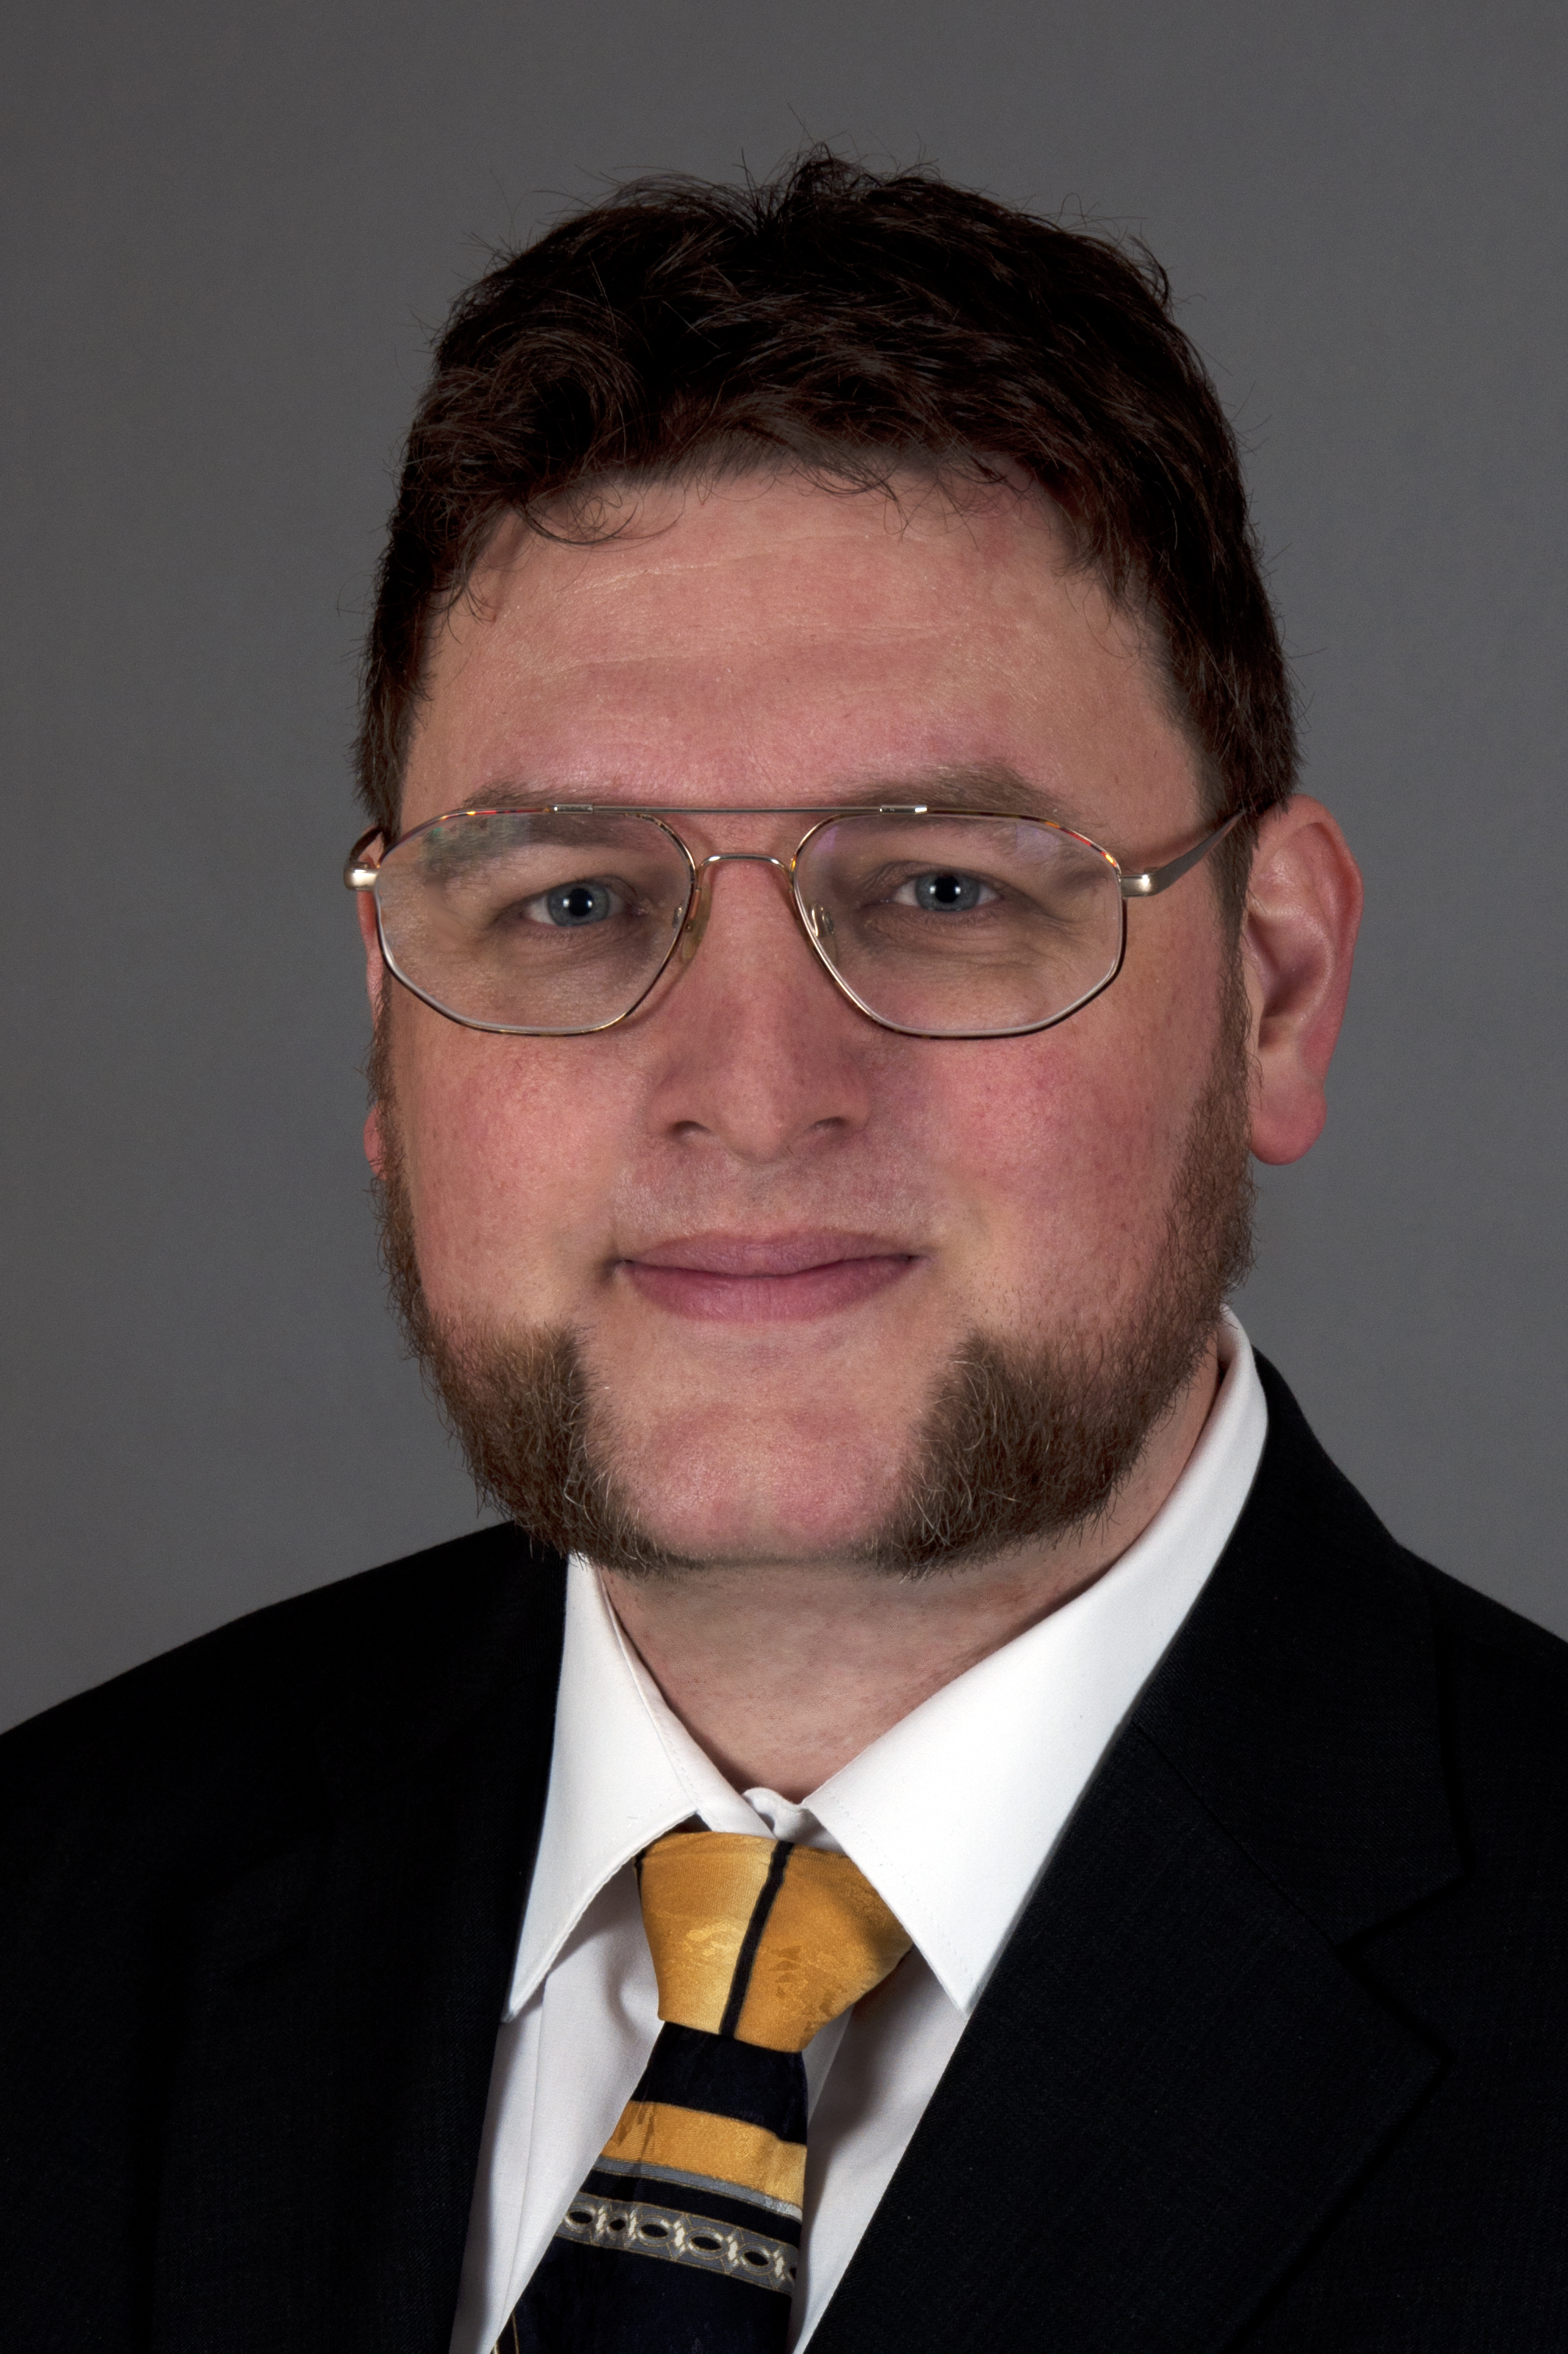
\includegraphics[width=0.29\columnwidth]{inc/biography/passphoto}
\end{wrapfigure}
% !TeX spellcheck = en_GB

Martin Gwerder was born 20. July 1972 in Glarus, Switzerland. He is currently a doctoral Student at the University of Basel. After having concluded his studies at the polytechnic at Brugg in 1997, he did a postgraduate study as a master of business and engineering. Following that, he changed to the university track doing an MSc in Informatics at FernUniversit\"at in Hagen. While doing this he constantly broadened his horizon by working for industry, banking and government as  engineer and architect in security related positions. He currently holds a lecturer position for cloud and security at the University of Applied Sciences Northwestern Switzerland. His main expertise lays in the field of networking related problems dealing with data protection, distribution, confidentiality and anonymity.
\end{document}